\documentclass[12pt, twoside]{report}
	\usepackage[margin=1in]{geometry}
	\usepackage[hidelinks, linktoc=all, pagebackref]{hyperref}
	\usepackage{indentfirst}
    \usepackage{subcaption}
   	\usepackage[superscript,biblabel]{cite}
    \usepackage[font=small,labelfont=bf]{caption}
    \usepackage{abstract}
    \usepackage{mathtools}
    \usepackage{cleveref}
    \usepackage{fancyhdr}
    \usepackage{enumitem}
    \setlength{\parskip}{0.1cm}   
	\setlength{\parindent}{0.7cm}
    \usepackage{graphicx} % Used to insert images
    \usepackage{adjustbox} % Used to constrain images to a maximum size 
   	\usepackage{color} % Allow colors to be defined
    \usepackage{geometry} % Used to adjust the document margins
    \usepackage{amsmath} % Equations
    \usepackage{amssymb} % Equations
    \usepackage[mathletters]{ucs} % Extended unicode (utf-8) support
    \usepackage[utf8x]{inputenc} % Allow utf-8 characters in the tex document
    \usepackage{fancyvrb} % verbatim replacement that allows latex
    \usepackage{grffile} % extends the file name processing of package graphics 
                         % to support a larger range 
    % The hyperref package gives us a pdf with properly built
    % internal navigation ('pdf bookmarks' for the table of contents,
    % internal cross-reference links, web links for URLs, etc.)
    \usepackage{longtable} % longtable support required by pandoc >1.10
\usepackage{bbm}

\newcommand{\diff}{\,\mathrm{d}} 	
 \renewcommand{\figureautorefname}{Fig.}%
\renewcommand*\thesection{\arabic{section}}
\DeclarePairedDelimiter\bra{\langle}{\rvert}
\DeclarePairedDelimiter\ket{\lvert}{\rangle}
\DeclarePairedDelimiterX\braket[2]{\langle}{\rangle}{#1 \delimsize\vert #2}
\newcommand{\rbrkt}[1]{\left( #1 \right)}
\newcommand{\sbrkt}[1]{\left[ #1 \right]}

\renewcommand*{\backreftwosep}{ and~}
\renewcommand*{\backreflastsep}{ and~}
\renewcommand*{\backref}[1]{}
\renewcommand*{\backrefalt}[4]{%
\ifcase #1 %
\relax%
\or
(referenced on p. [#2])%
\else
(referenced on p. [#2])%
\fi
}

\numberwithin{equation}{section}
\setcounter{tocdepth}{3}

\renewcommand*\thesection{\arabic{chapter}.\arabic{section}}
\lhead[\rm\thepage]{\fancyplain{}{\nouppercase{\sl{\rightmark}}}}
\rhead[\fancyplain{}{\nouppercase{\sl{\leftmark}}}]{\rm\thepage}
\chead{}\lfoot{}\rfoot{}\cfoot{}
\pagestyle{fancy}

\title{Reverse engineering of the Xmon qubits}

\graphicspath{{Pictures/}, {MIPT NIR presentation/Pics/}}


\begin{document}
\maketitle
\tableofcontents

\chapter{Theoretical introduction}

\section{Superconducting microwave coplanar waveguide resonators}

\subsection{Equations for quality factors}

The total quality factor of a microwave transmission line resonator (TLR) $Q_l$ (loaded quality factor) can be calculated as a sum of two parts -- the internal and external quality factors. The internal quality factor $Q_i$ describes how excitations leave the resonator in the absence of coupling to any external circuitry, so damping in this case comes from the internal defects (i.e. resonant two-level systems) in the resonator itself. When, however, the resonator is coupled to the external circuitry having some active resistance, the damping is enhanced and the total Q-factor is reduced according to the following expression:
\begin{equation}
Q_l^{-1} = Q_i^{-1}+Q_e^{-1},
\label{eq:qfactor}
\end{equation}
where $Q_e$ is determined by the value of the externally connected resistance and the way of its connection.

\begin{figure}
\captionsetup[subfigure]{width = 0.9\textwidth, justification=normal}
\centering
\begin{subfigure}[t]{0.48\textwidth}
\centering
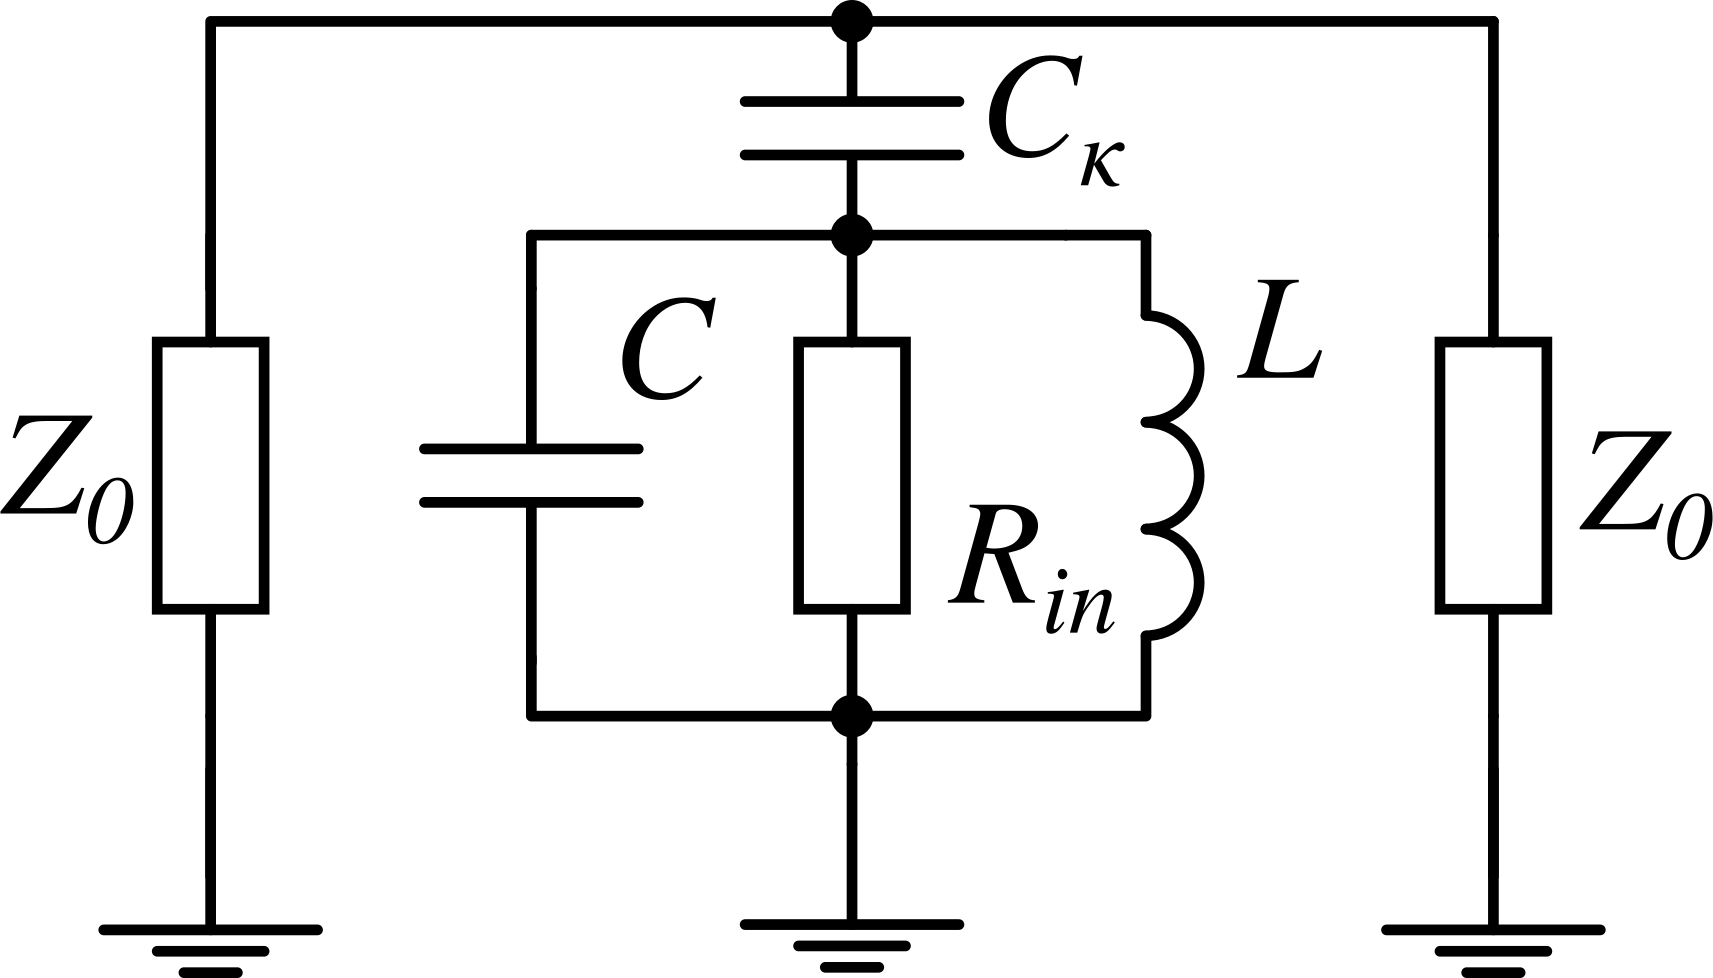
\includegraphics[width=0.9\textwidth]{resonator}
\caption{Real world circuit configuration.}
\end{subfigure}
\begin{subfigure}[t]{0.48\textwidth}
\centering
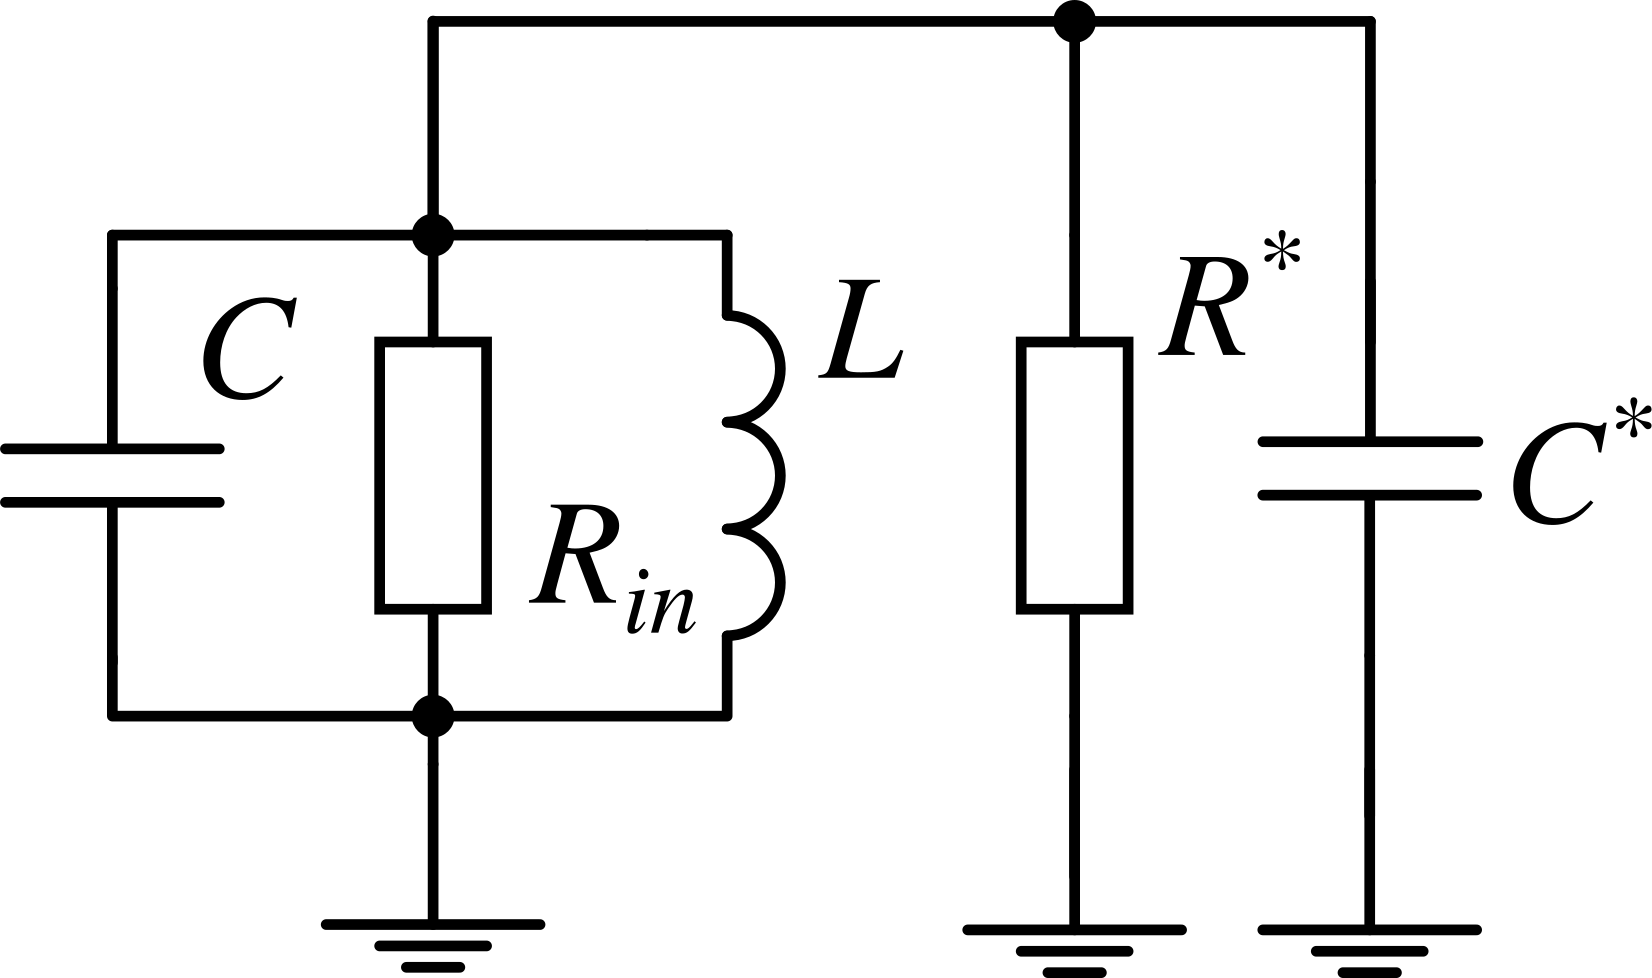
\includegraphics[width=0.9\textwidth]{resonator_equiv}
\caption{Norton equivalent of (a).}
\end{subfigure}

\caption{Equivalent circuit for a $\lambda/4$ TLR, capacitively coupled to the transmission line near resonance.}
\label{fig:resonator_equiv}
\end{figure}

A common way of measuring a resonator is to couple it capacitively to an external transmission line. The coupling on the equivalent scheme of the circuit is represented as $C_\kappa$, as depicted in \autoref{fig:resonator_equiv}~(a). An infinite/properly terminated transmission line can be represented as a single resistance of $Z_0$ Ohms, where $Z_0$ is the line's wave impedance; thus, two such resistances are added to the both sides of the resonator circuit. The resonators are of $\lambda/4$ type, so the equivalent for each of them is a parallel RLC oscillator (see below), where $C$ and $L$ are, respectively, its equivalent capacitance and inductance and $R=R_{in}$ characterises the internal dissipation. Its $Q_i  = \omega_0 C R_{in}$ where $\omega_0 = \sqrt{1/LC}$ can be calculated from the definition when no external impedance is connected.
 
The external Q-factor can be derived in a bit more complicated way\cite{Goppl2008}. We can transform the circuit from the \autoref{fig:resonator_equiv}~(a) to explicitly include the external parameters into the internal ones. To do so one needs to convert the series connection of the coupling capacitor and the characteristic impedances into parallel, as done on the \autoref{fig:resonator_equiv}~(b). The $R^*$ and $C^*$ impedances should be chosen in such a way that total impedance of the external circuit is the same as before the transformation:
\begin{align}
R^{*} &= \frac{1+\omega^2 C_\kappa^2 (Z_0/2)^2}{\omega^2 C_\kappa^2 (Z_0/2)	}, \\
C^{*} &= \frac{C_\kappa}{1+\omega^2 C_\kappa^2 (Z_0/2)^2} \approx C_\kappa\ (\text{in our case}). \label{eq:C_ast}
\end{align}
From this and \autoref{fig:resonator_equiv}~(b) it is simple to write down the expression for the internal, external and loaded quality factors:
\begin{gather}
Q_i =  \omega (C+C^{*}) R_{in}, \\
Q_e = \omega (C+C^{*}) R^{*}, \\
Q_l = \omega (C+C^{*})  \frac{1}{1/R^{*}+1/R_{in}}. \label{eq:Q_l}
\end{gather}
The above expressions readily justify \eqref{eq:qfactor}. The values been used in the simulations are: $C = 350$ fF, $L = 2$ nH, $R_{in}=10^7$ Ohm, $Z_0 = 50$ Ohm. 


\begin{figure}
\centering
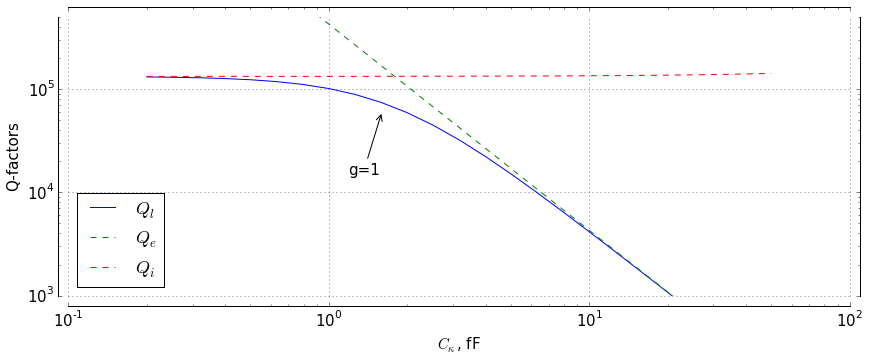
\includegraphics[width=0.9\textwidth]{q-factors}
\caption{Q-factors dependence on $C_\kappa$ according to \eqref{eq:Q_l}.}
\end{figure}


\subsubsection{The lumped-element model of a coplanar waveguide resonator}\label{ssec:LE-model}
A $\lambda/4$ coplanar waveguide (CPW) resonator near a resonance is equivalent to a lumped-element parallel resonance circuit, as in \autoref{fig:resonator_equiv}. $L$ and $C$ for the lumped-element models of CPW resonators are bound not only by the resonance frequency condition $\omega_0 = 1/\sqrt{LC}$ but also by the geometry of the waveguide or, in other words, $C^\prime$ and $L^\prime$ -- the transmission line capacitance and inductance per unit length. To show this, one would write down the impedance of the CPW resonator near its resonance frequency $\omega_0$ and compare it to the lumped-element one's\cite{pozar2012}. Such comparison leads to the following expressions:
\[
R_{in} = \frac{Z_0}{\alpha l}, \quad C = \frac{\pi}{4\omega_0 Z_0},
\]
where $l$ is the resonator length, $Z_0 = \sqrt{L^\prime/C^\prime}$ is the wave resistance and $\alpha$ is the decay constant of the line. Then the resonance condition for the wavelength ($\lambda = 4 l$) is used along with the phase velocity expression $v_{ph} = 1/\sqrt{L^\prime C^\prime}$:
\[
\omega_0 = \frac{2\pi v_{ph}}{\lambda} =  \frac{\pi \, v_{ph}}{2 l} \Rightarrow  C = \frac{C^\prime l}{2}.
\]
For the inductance one can use $L = 1/\omega_0^2 C = 8 l\, L^\prime/\pi^2$. Finally, the expressions for $C^\prime$ and $L^\prime$:
\[
C^\prime = 4\varepsilon_0\varepsilon_{eff} \frac{K(k_0)}{K(k_0^\prime)},\quad
L^\prime = \frac{\mu_0}{4} \frac{K(k_0^\prime)}{K(k_0)},
\]
where $K(x)$ is the complete elliptic integral of the first kind, $\varepsilon_{eff} = \frac{1+\varepsilon_{substrate}}{2}$, $k_0 = \frac{W}{W+2G}$ where $W$ is the width of the hotwire and $G$ is the width of the gaps and finally $k_0^\prime = \sqrt{1-k_0^2}$.

\subsection{S-parameters for lines with resonators}

Typically, a microwave device under test (DUT) is tested with a vector network analyser, which measures the scattering matrix (S-matrix) of the DUT. So below we will discuss the S-matrix for two different coupling configurations. Generally, a two-port DUT can be drawn like in \autoref{fgeneral2port}. For such system it is possible to calculate different 2 by 2 matrices, which bind together voltages and currents on the ports 1 and 2. S-matrix also has 4 values, named S-parameters.

\begin{figure}[h]
\centering
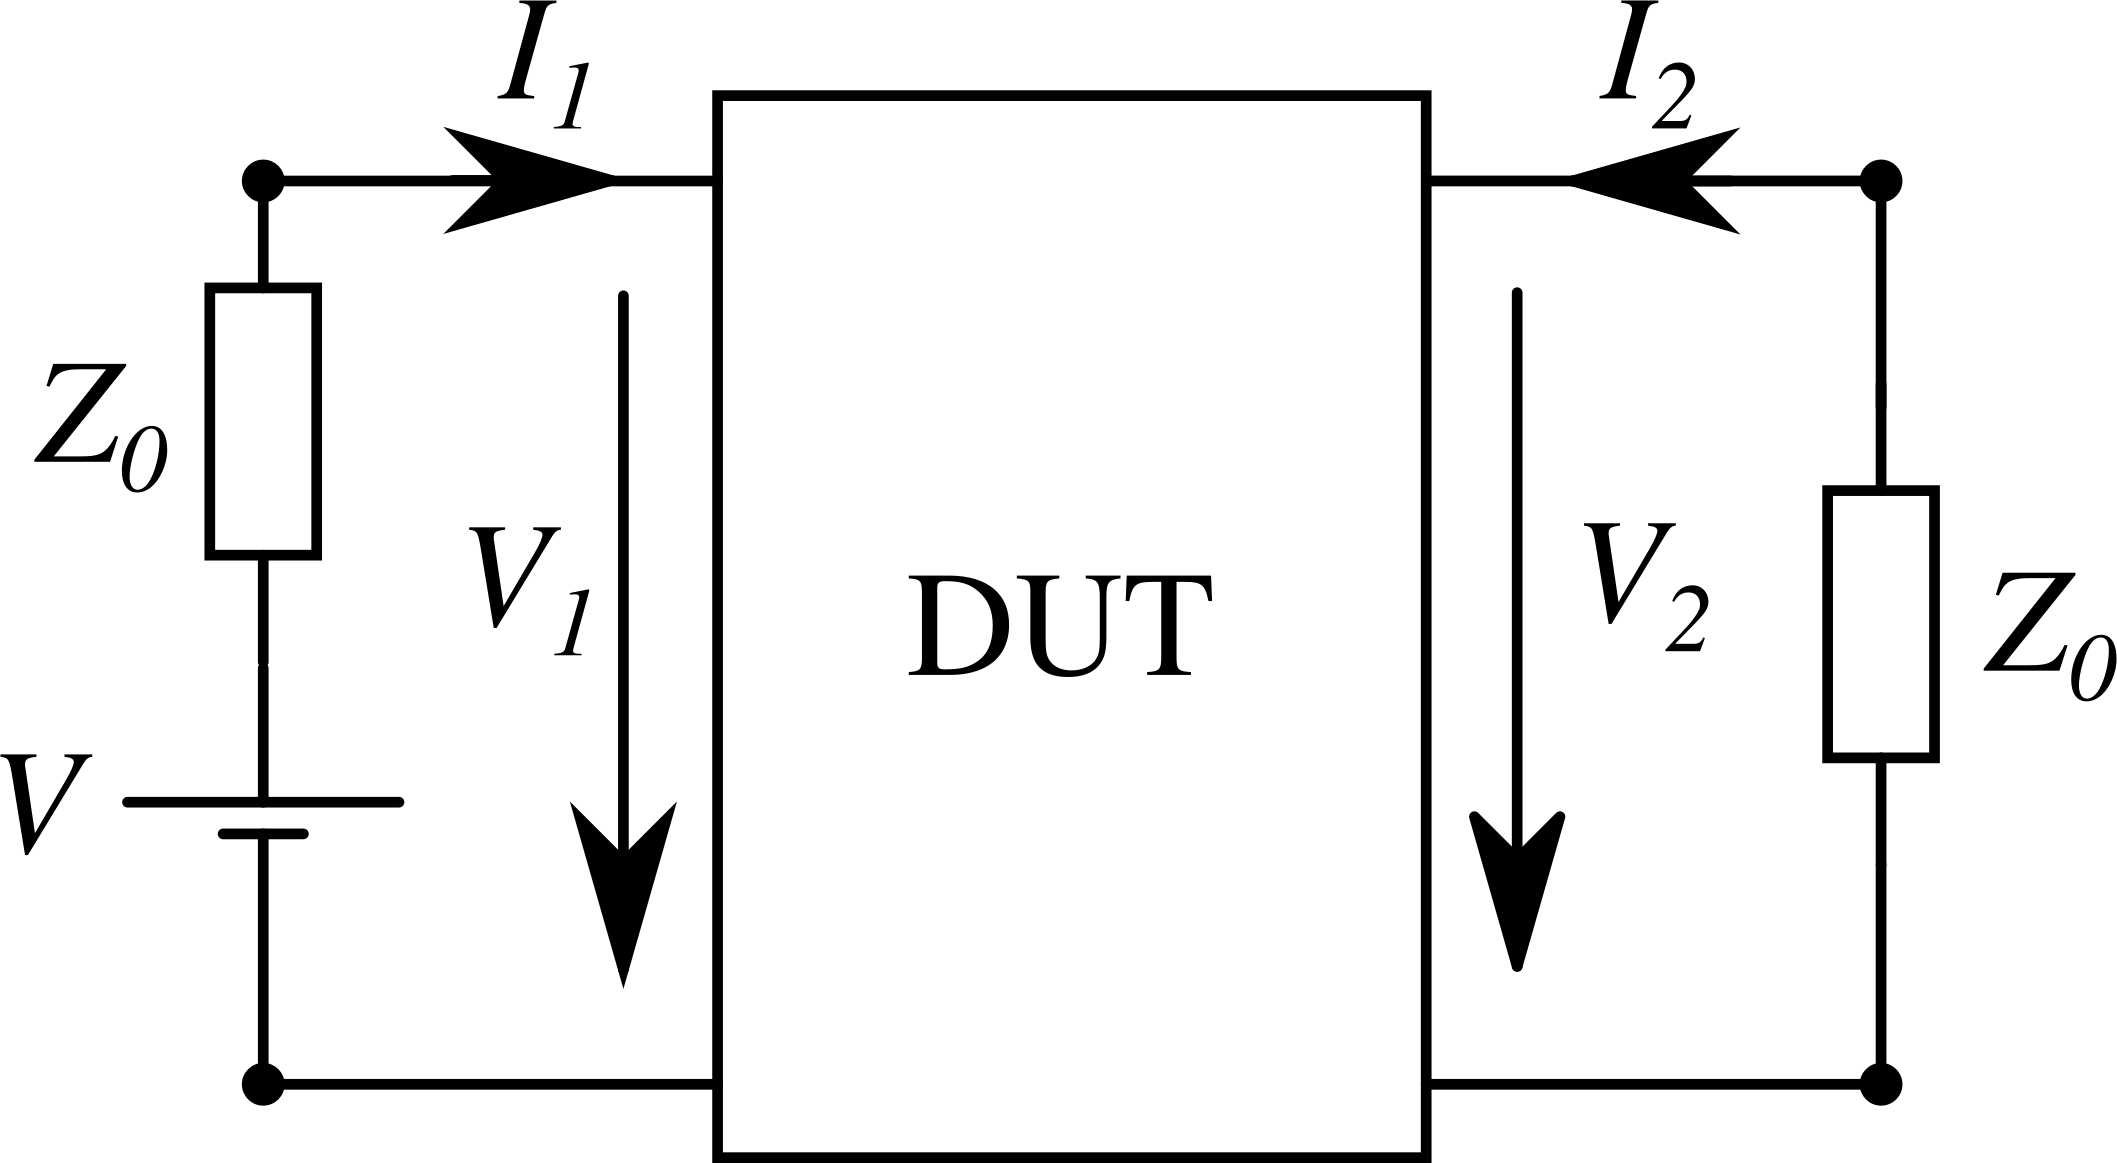
\includegraphics[width=0.5\textwidth]{tl_scheme_general}
\caption{A scheme for the two-port network.}
\label{fgeneral2port}
\end{figure}

To calculate S-parameters one needs to treat voltages and currents, which can be calculated from Kirchhoff's laws, as a sum of the incident and reflected components (``+'' corresponds to the incident wave and ``$-$'' to the reflected wave):
\begin{gather*}
V_{1,2} = V_{1,2}^+ + V_{1,2}^- ,\\
I_{1,2} = I_{1,2}^+ + I_{1,2}^- = \frac{ V_{1,2}^+ - V_{1,2}^- }{Z_0},
\end{gather*}
where the difference in the second expression arises from telegrapher's equations. Solving these with respect to incident and reflected components, one can get
\begin{equation*}
V_{1,2}^\pm = \frac{1}{2}(V_{1,2} \pm Z_0 I_{1,2}).
\end{equation*}
From this, finally, S-parameters are defined:
\begin{equation}
\rbrkt{\begin{matrix}
V_1^- \\
V_2^-
\end{matrix}} = 
\rbrkt{\begin{matrix}
S_{11} & S_{12} \\
S_{21} & S_{22}
\end{matrix}}
\rbrkt{\begin{matrix}
V_1^+ \\
V_2^+
\end{matrix}}.
\label{eq:S_def}
\end{equation}
However, it's often more convenient to use indirect methods of calculating S-parameters, for example, to extract them from $ABCD$-matrix.




\subsection{Coupled (shunting) design}
For a coupled design one can treat the resonator as a shunt in the transmission line as in \autoref{fig:shunted_tl}. Except than by the definition \eqref{eq:S_def} there are two other ways to calculate the S-matrix. First one is intuitive but is not valid for every configuration. Transmission and reflection parameters are defined\cite{Kiselev2013} below (the second formula is valid only for the ``shunt'' configuration, no series elements are allowed in the line):
\begin{gather}    
\Gamma = \frac{Z_{eff} - Z_{0}}{Z_{eff} + Z_{0}} = S_{11} = S_{22}, \label{eGamma}\\
T = \frac{2Z_{eff}}{Z_{eff}+Z_0} \overset{!}{=} S_{21} = S_{12}, \label{eT}
\end{gather}
where $Z_{eff} = Z_0 || Z_{shunt}$, $Z_{shunt} = \frac{1}{i\omega C_\kappa} + 1/i\omega C||R_{in}||i\omega L$ and the equalities between S-parameters hold due to the symmetry.
\begin{figure}[h]
\centering
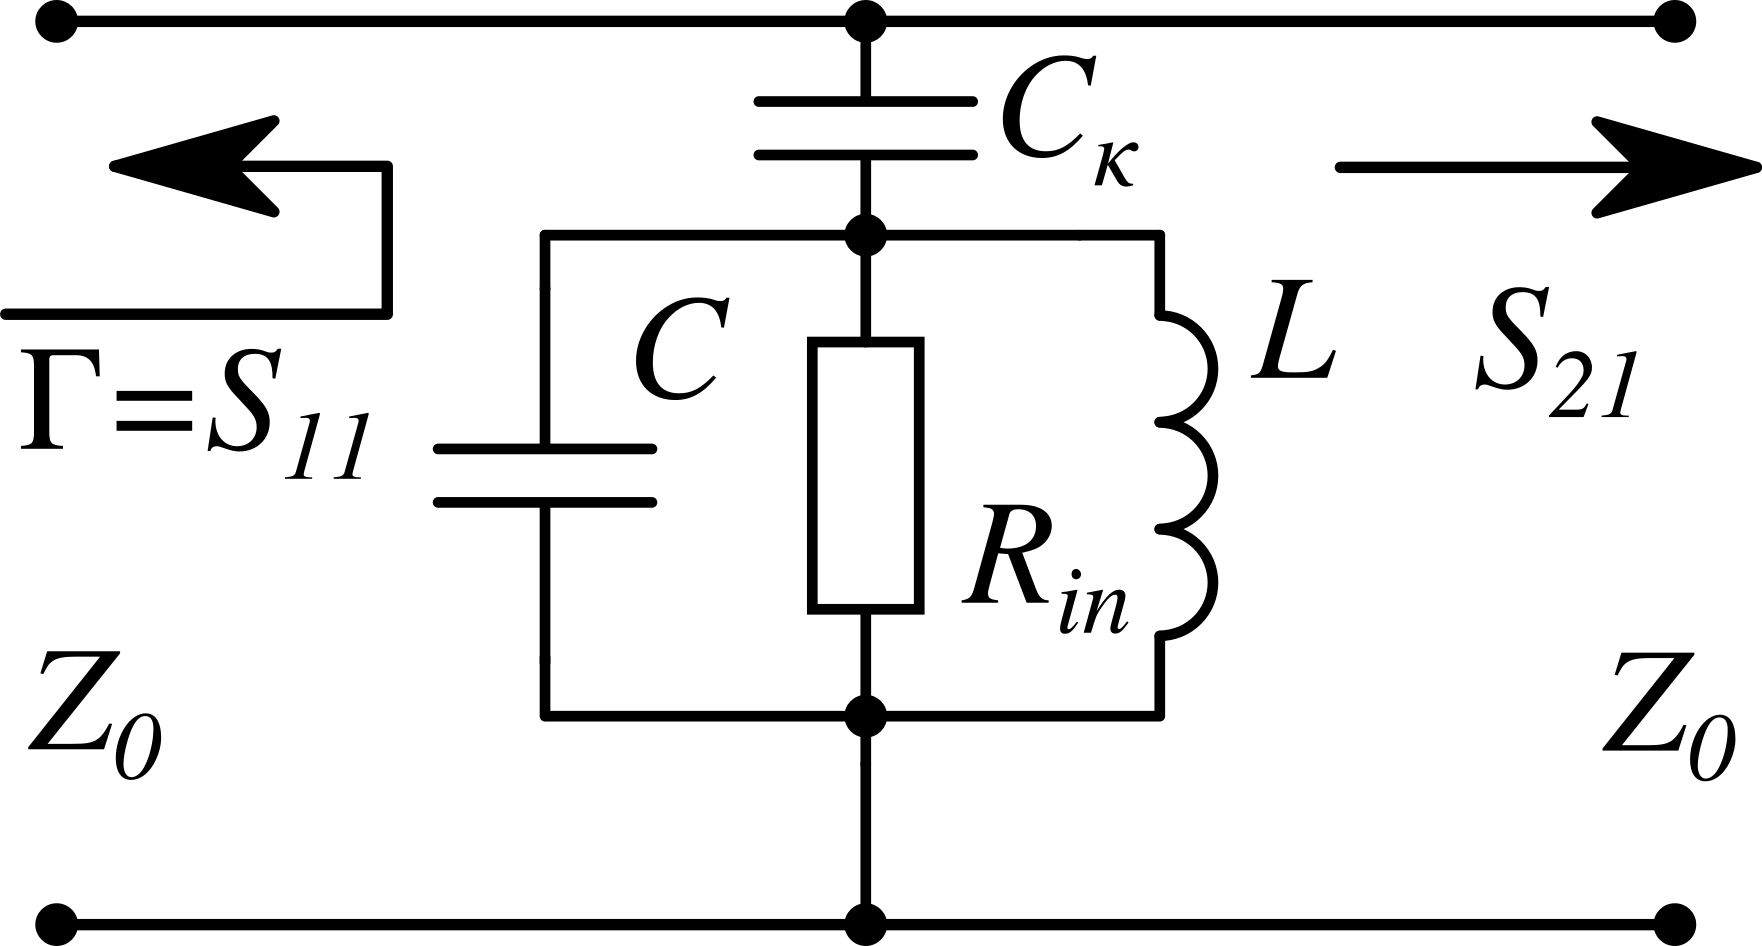
\includegraphics[width=0.5\textwidth]{tl_scheme}
\caption{The shunted transmission line. This is \autoref{fig:resonator_equiv}~(a)  from the observer's point of view.}
\label{fig:shunted_tl}
\end{figure}
\begin{figure}[h]
\centering
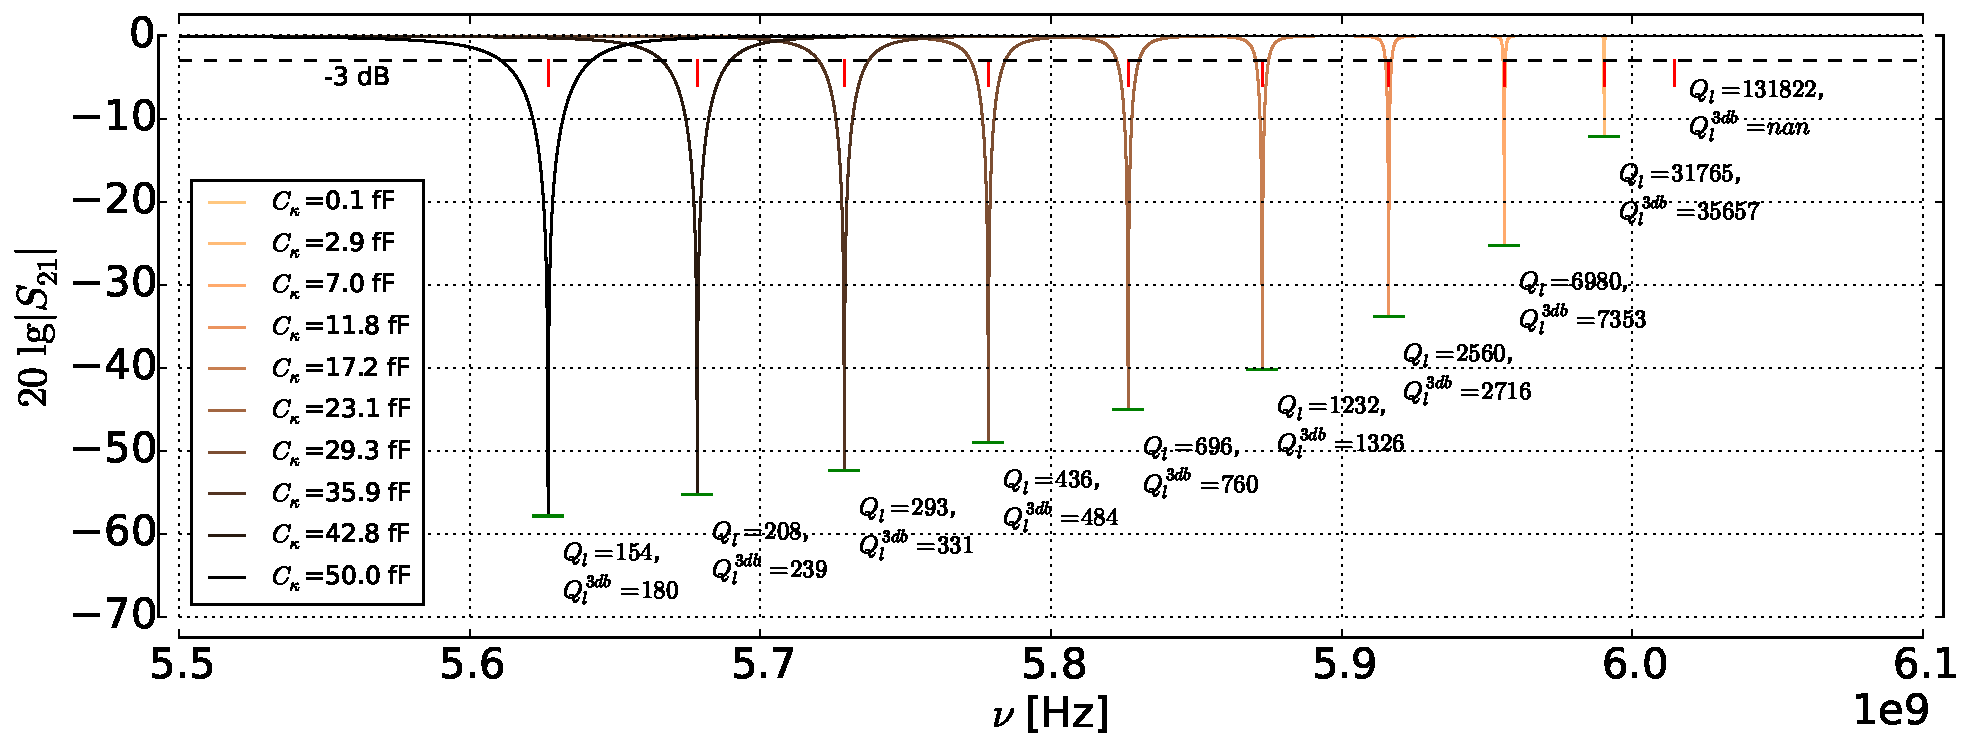
\includegraphics[width=0.99\textwidth]{S21s}
\caption{ $S_{21}$ parameters from \eqref{eq:S21} for different coupling strengths. The loaded quality factors are calculated with \eqref{eq:Q_l} and with the ``3db''-method. The red dashes show the values of expression $\sqrt{1/L(C+C_k)}$ according to \autoref{fig:resonator_equiv}~(b), the green ones show the theoretically predicted depths.}
\label{fig:S21s}
\end{figure}

Another way is to calculate $ABCD$ matrix or impedance matrix and convert it to the S-matrix with corresponding formulae\cite{pozar2012}. In the ``shunted'' case from both this approaches the simplified expressions for the S-parameters follow:
\begin{gather}
S_{11} = -\frac{Z_0}{1 + 2Z_{shunt}/Z_0} = S_{22}, \\
S_{21} = \frac{1}{1+Z_0/2Z_{shunt}} = S_{12}. \label{eq:S21}
\end{gather}
The second expression is plotted in \autoref{fig:S21s} along with the loaded quality factors calculated with \eqref{eq:Q_l} and with the ``3db''-method ($Q_L \approx \omega_0/\Delta\omega_{3db}$). It can be seen that with increase of capacitance resonance frequency and $Q_l$ decrease, which is expected according to \autoref{fig:resonator_equiv}~(b) and \eqref{eq:C_ast}.

In \autoref{fig:S21s} the resonance frequencies calculated from the equivalent circuit in \autoref{fig:resonator_equiv}~(b) are shown along with the analytically calculated depths of the peaks:
\begin{equation}
\min_f S_{21} = \frac{2 L \left(C + C_{\kappa}\right)}{\sqrt{C_{\kappa}^{2} L Z_{0}^{2} \left(C + C_{\kappa}\right) + \left(2 (C+C_\kappa) L + C_{k}^{2} R_{in} Z_{0} \right)^{2}}}.
\end{equation}

\subsection{Embedded (series) design}

For the embedded resonator it's possible to draw a similar equivalent circuit as for the ``shunt'' design\cite{Goppl2008}. It is depicted in \autoref{fseries_tl}. 

\begin{figure}[h]
\centering
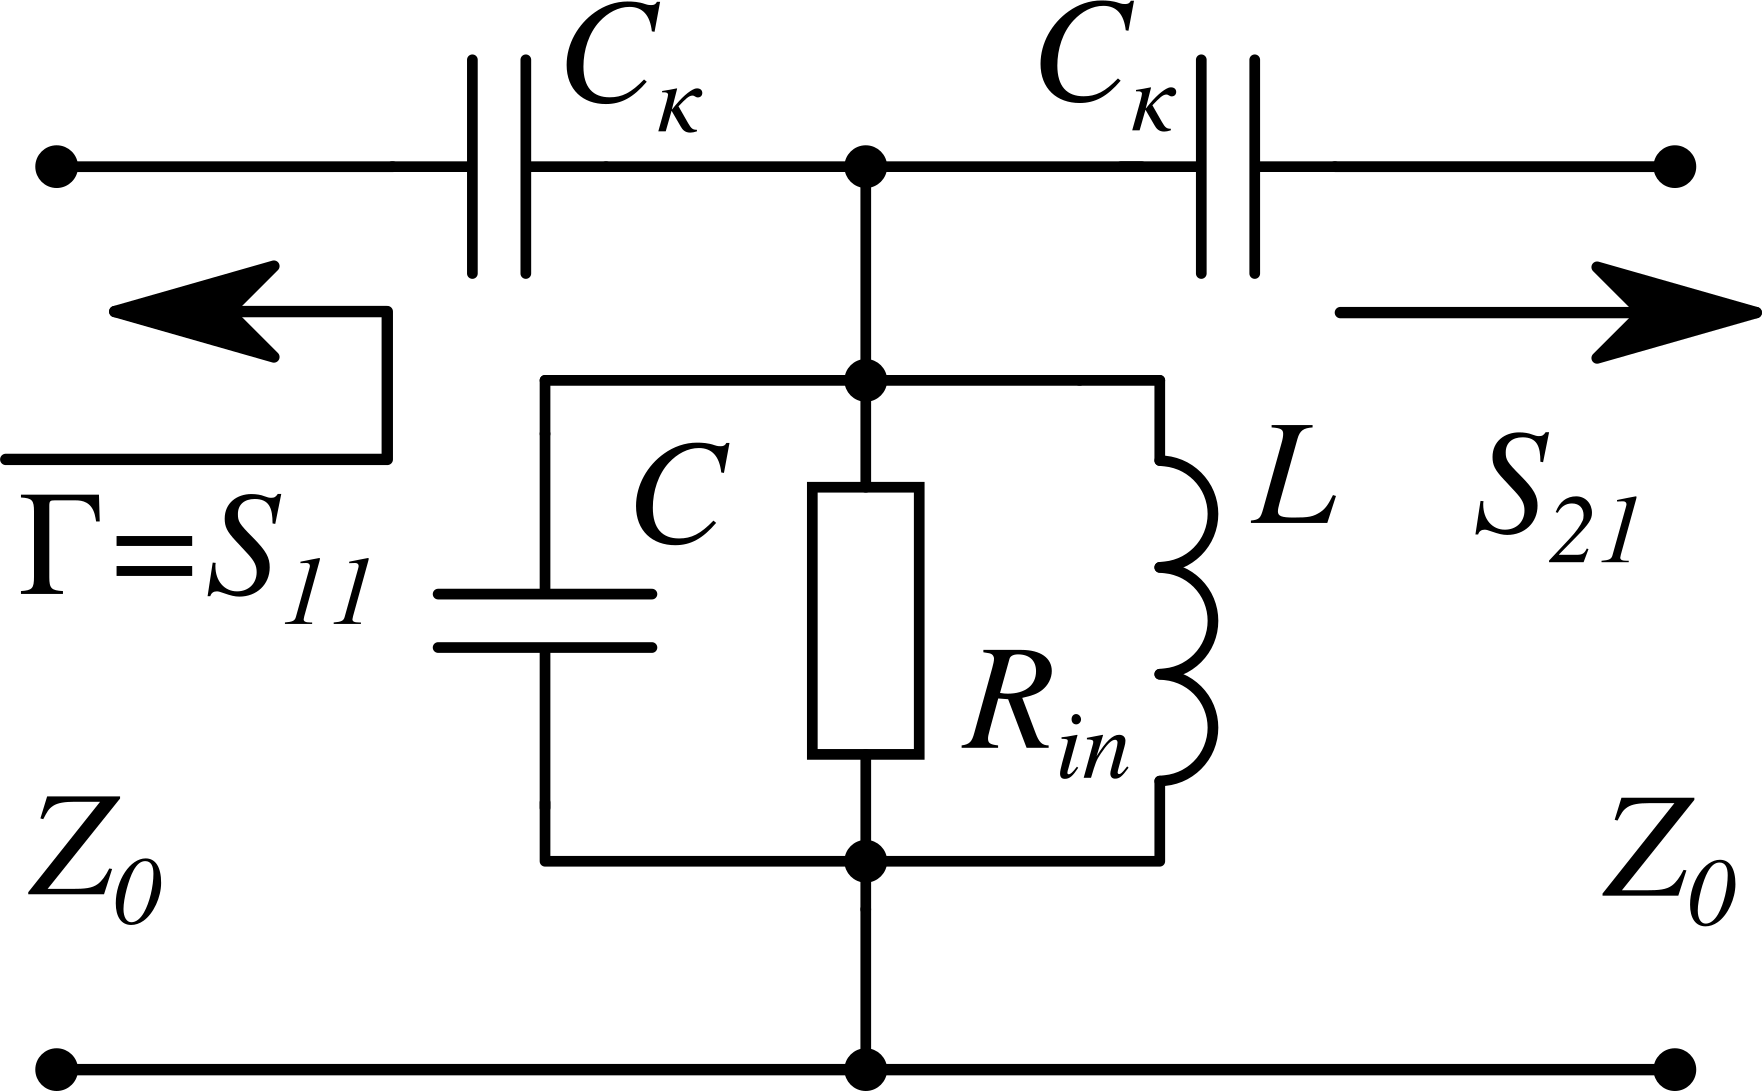
\includegraphics[width=0.5\textwidth]{tl_scheme_series}
\caption{The equivalent circuit for the embedded resonator.}
\label{fseries_tl}
\end{figure}
\begin{figure}[h]
\centering
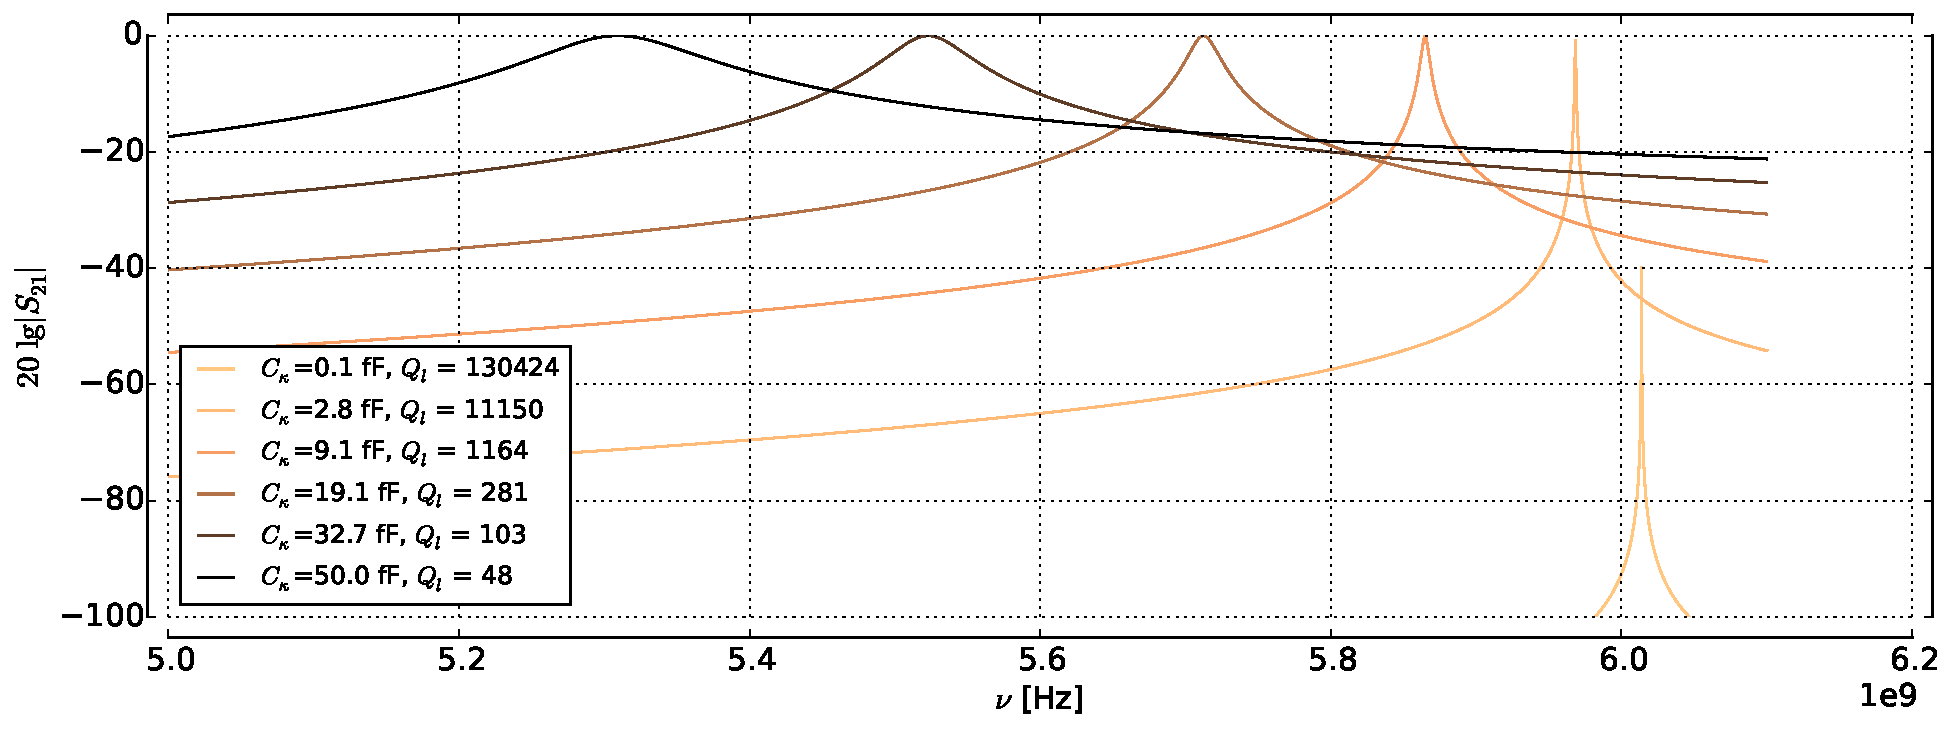
\includegraphics[width=0.9\textwidth]{S21s_series}
\caption{$S_{21}$ for the series configuration. Loaded Q-factors were calculated  via analytic expression similar to \eqref{eq:Q_l}.}
\label{fS21s_series}
\end{figure}

For this kind of connection of the resonator to the transmission line \eqref{eT} is now not valid (however, \eqref{eGamma} still holds). To calculate transmission in this case one may find the transmission matrix and then convert it to the S-matrix or use Kirchhoff's laws and \eqref{eq:S_def}. For studied case one can get the following $ABCD$-matrix\cite{pozar2012}
\begin{equation}
\hat T = \rbrkt{\begin{matrix}
A & B \\
C & D
\end{matrix}} = \rbrkt{\begin{matrix}
1 + \frac{1/i\omega C_\kappa}{Z_{res}} & 2/i\omega C_\kappa - \frac{\omega^2 C_\kappa^2}{Z_{res}} \\
1/Z_{res} &  1 + \frac{1/i\omega C_\kappa}{Z_{res}} 
\end{matrix}},
\end{equation}
where $Z_{res} = R_{in}||i\omega L || 1/i\omega C$. The corresponding $S_{21}$ is plotted in \autoref{fS21s_series}, calculated as\cite{pozar2012} 
\begin{equation}
S_{21} = \frac{2}{A+B/Z_0 +CZ_0 + D}.
\end{equation}

\section{Cirquit QED with transmons}\label{sec:cQED}


\subsection{Hamiltonian for the compound system}

Here we will use the results acquired by Bader\cite{Bader2013} and Koch\cite{Koch2007}. Using \autoref{fig:xmon-resonator} it is possible to obtain the quantized Hamiltonian for the compound circuit:

\begin{equation}
\begin{gathered}
\mathcal{\hat H} =  \underbrace{\frac{\hat \phi_r^2}{2 L_r} + \frac{(C_q+C_g) \hat Q_r^2}{2C_*^2}}_\text{resonator} 
+ \underbrace{\frac{(C_g + C_\kappa + C_r) \hat Q^2_q}{2C_*^2} - E_J (\Phi_{ext}) \cos \frac{2e}{\hbar}\hat \phi_q }_\text{qubit}
+ \underbrace{\frac{C_g\hat Q_r \hat Q_q}{C_*^2}}_\text{coupling} = \\
=  \hbar\omega_r\ \hat a^\dag \hat a \otimes \mathbbm{\hat 1}_q \quad (\mathcal{\hat H}_r) \\
+ 4 E_C\ \mathbbm{\hat 1}_r \otimes \hat n^2 - \frac{E_J(\Phi_{ext})}{2}\ \mathbbm{\hat 1}_r\otimes \sum_{n=-\infty}^{+\infty} \ket{n+1}\bra{n} + \ket{n}\bra{n+1} \quad (\mathcal{\hat H}_q) \\
- 2e \frac{C_g}{C_*} \sqrt{\frac{\hbar \omega_r }{2(C_q+C_g)}}\ i(\hat a^\dag - \hat a) \otimes \hat n, \quad (\mathcal{\hat H}_i)
\end{gathered}\label{eq:hamiltonian}
\end{equation}
where 
$$C_*^2 = C_q C_g + C_q C_\kappa + C_g C_\kappa + C_q C_r + C_g C_r, $$
$$\omega_r = 1/\sqrt{L_r C_*^2/(C_q+C_g)}, $$
$$E_C = \frac{(C_g+C_\kappa+C_r)e^2}{C_*^2}, $$
$$E_J(\Phi_{ext}) = E_{J,\Sigma} \cos(\Phi_{ext}/\Phi_0),\ \Phi_{ext} = I_\Phi M.$$
Presuming the coupling is not very strong ($C_g \ll C_q, C_r$) it is possible also to include simple time-dependent driving terms for both subsystems:
\begin{gather}
\mathcal{\hat H}_r^d(t) = \frac{C_\kappa V_\kappa(t)}{C_r + C_\kappa} \hat Q_r \propto f_r(t)\ i(\hat a^\dag - \hat a) \otimes \mathbbm{\hat 1}_q, \notag \\
\mathcal{\hat H}_q^d(t) = \frac{C_e V_e(t)}{C_q + C_e} \hat Q_q \propto f_q(t)\  \mathbbm{\hat 1}_r \otimes \hat n,
\label{eq:driving_q}
\end{gather}
where $f_{q, r} (t)$ are the effective values of the drive magnitude at time $t$.

\begin{figure}
\centering
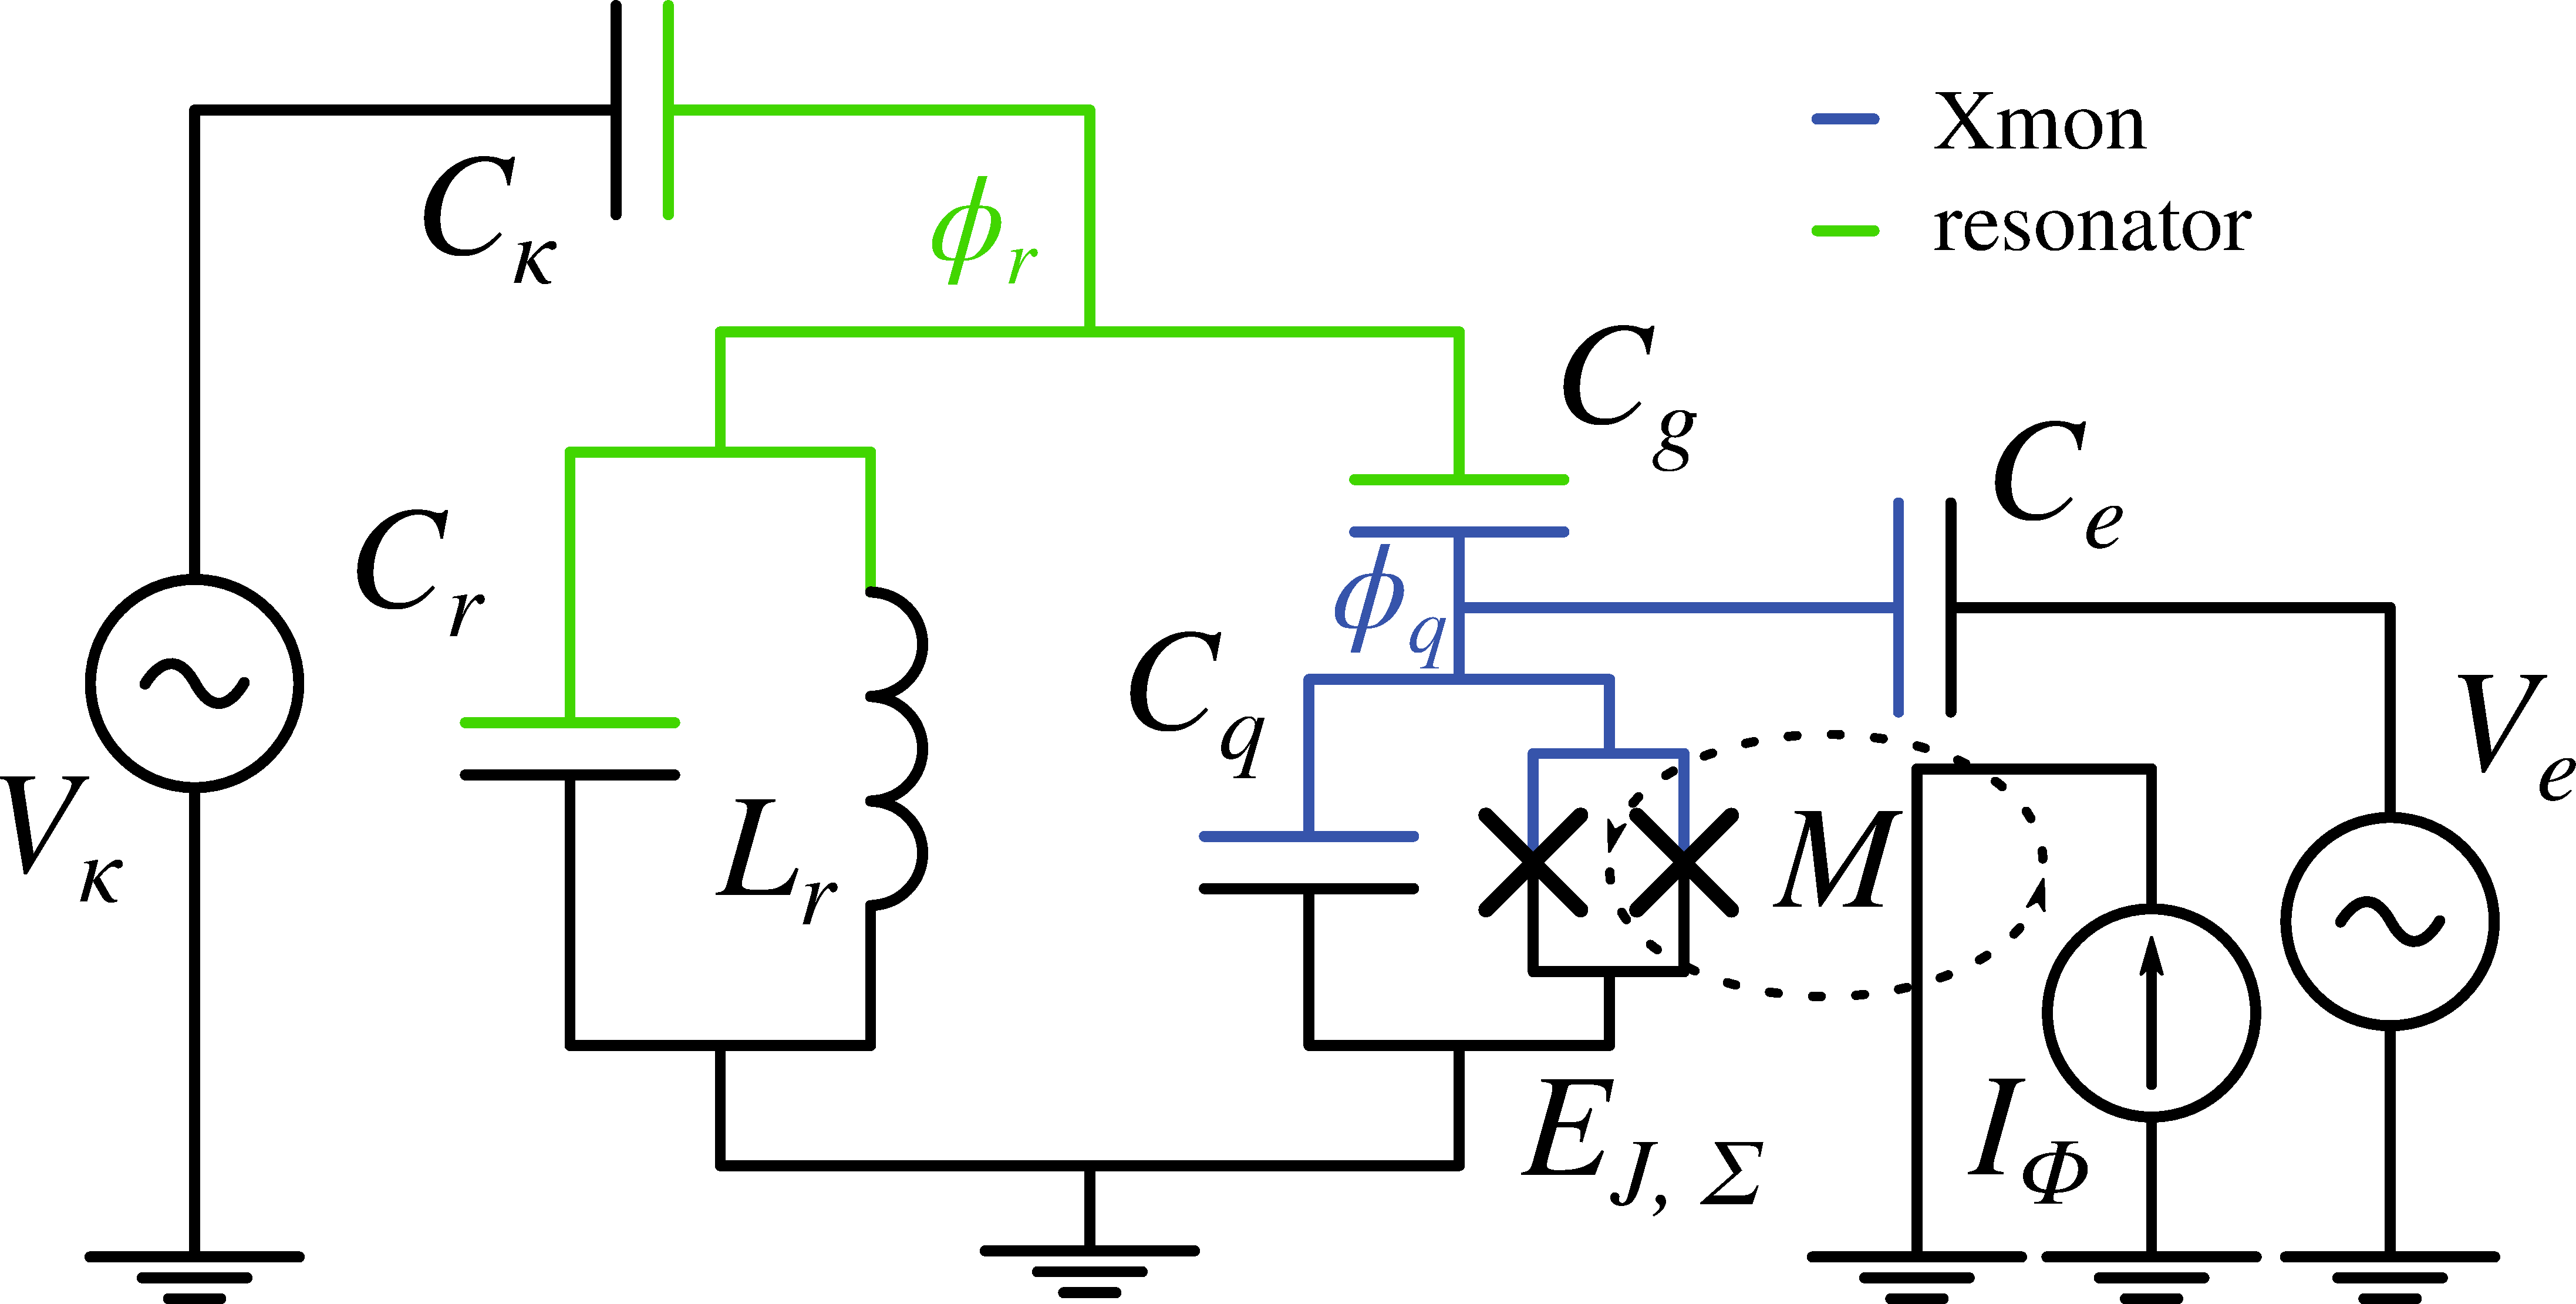
\includegraphics[width=0.8\textwidth]{xmon-resonator}
\caption{Equivalent circuit for coupled system of a tunable transmon qubit and a resonator. Colors show nodes (or branches) containing system's degrees of freedom according to M. Devoret's theory\cite{Devoret1995}.}
\label{fig:xmon-resonator}
\end{figure}
\begin{figure}
\centering
\begin{subfigure}[t]{\textwidth}
\centering
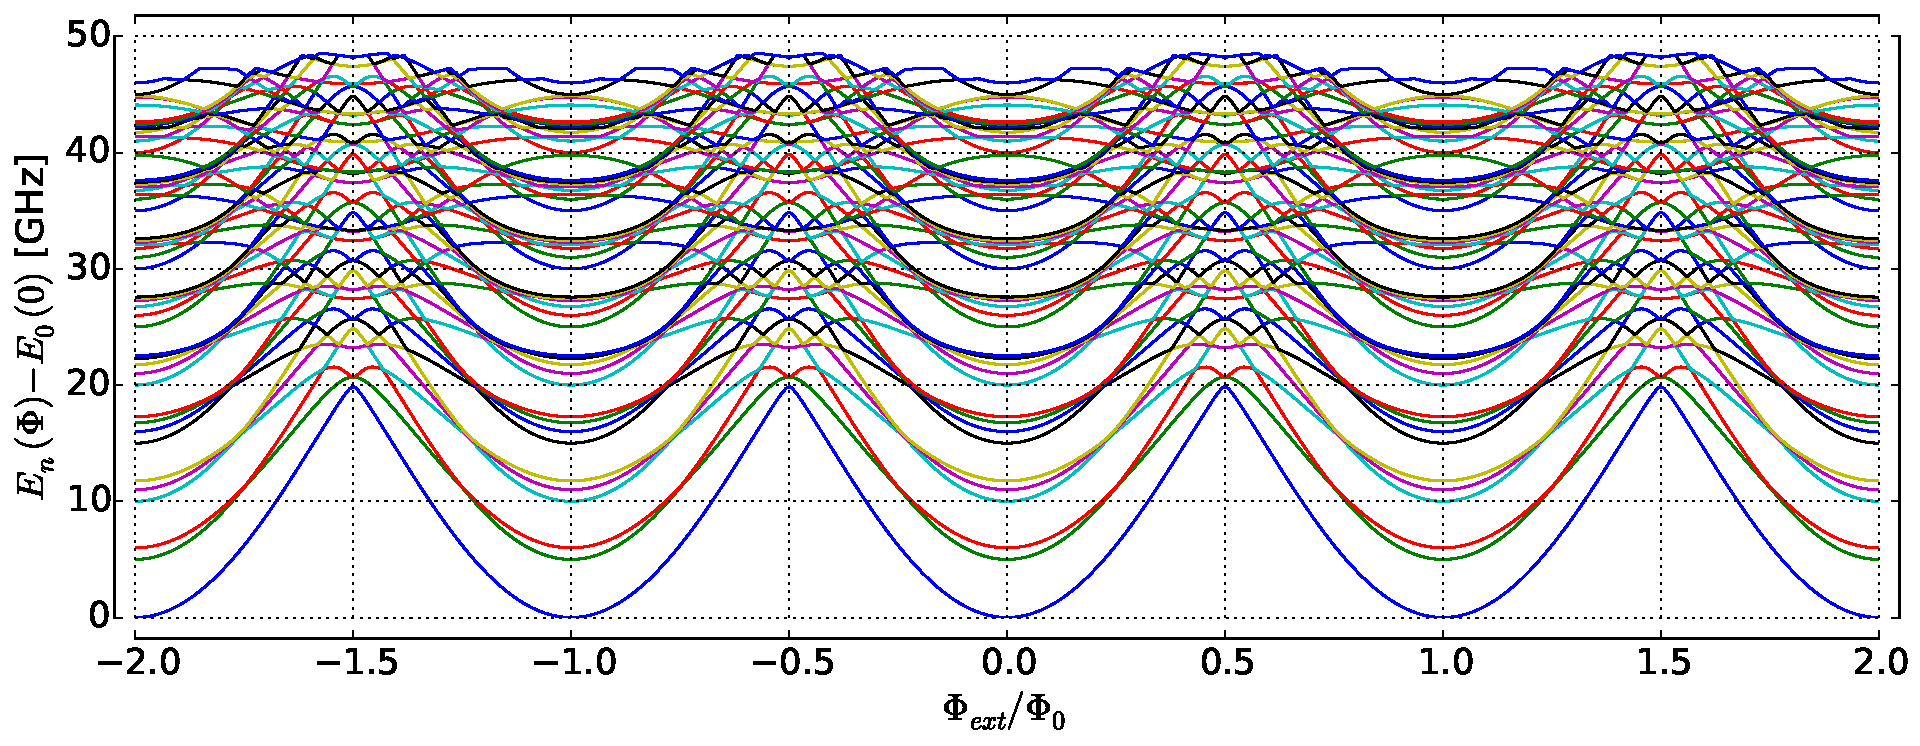
\includegraphics[width=0.9\textwidth]{levels}
\end{subfigure}

\begin{subfigure}[t]{\textwidth}
\centering
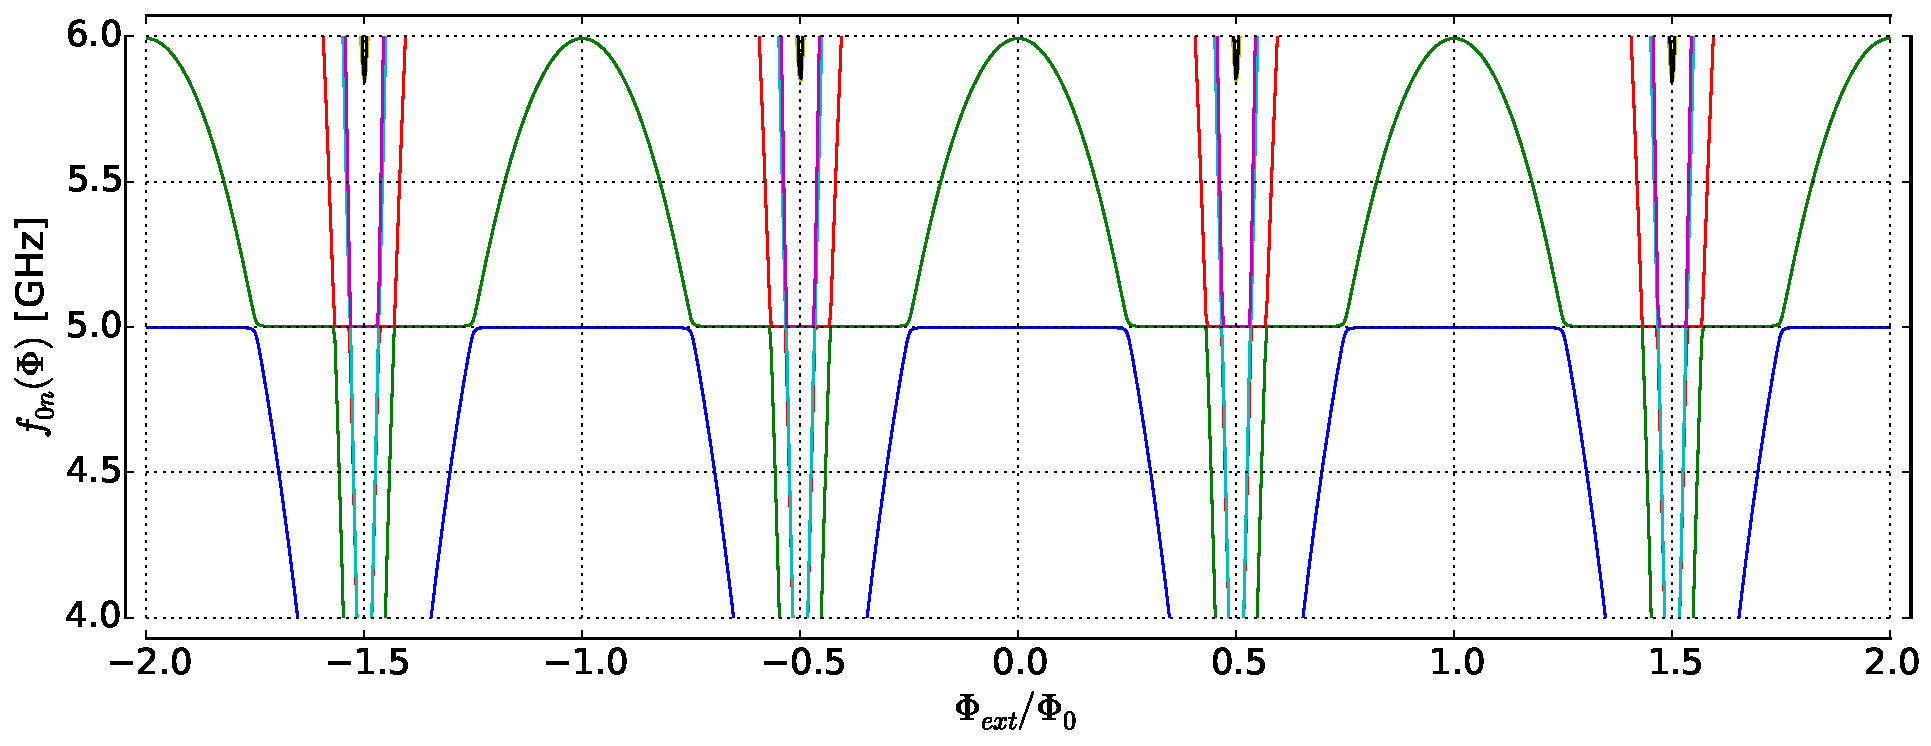
\includegraphics[width=0.9\textwidth]{freqs}
\end{subfigure}
\caption{Energy structure of the studied system depending on $\Phi_{ext}$.}
\label{fig:levels}
\end{figure}


\begin{figure}[h]
\centering
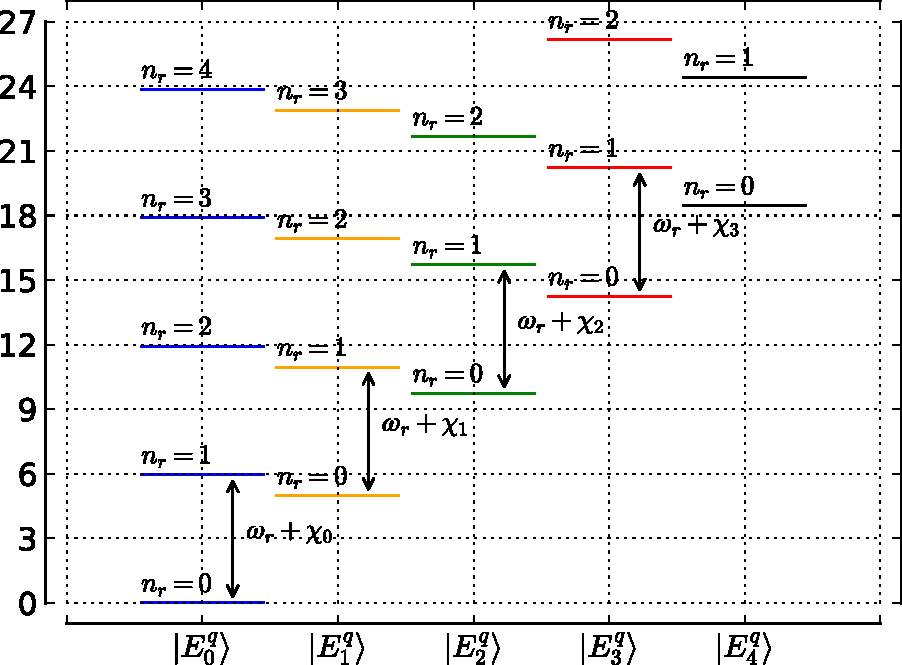
\includegraphics[width=\textwidth]{diagram_q<r}
\caption{Energy level diagram for the transmon-resonator system in the sweet spot when the detuning $\Delta_\omega = \omega_r-\omega_{ge}$ is positive.}
\label{fig:diagram}
\end{figure}

\begin{figure}[h]
\centering
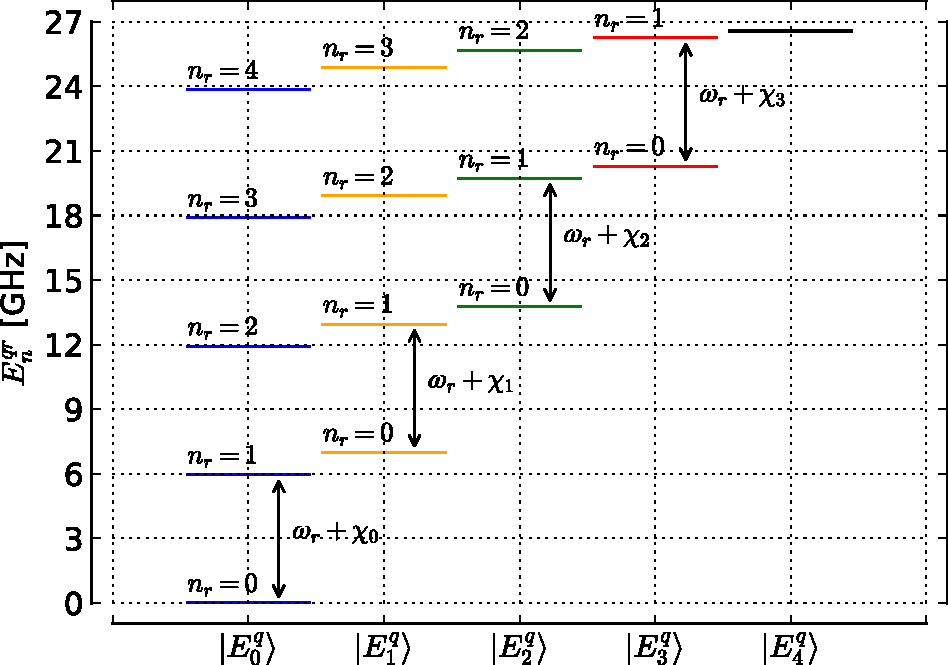
\includegraphics[width=\textwidth]{diagram_q>r}
\caption{Energy level diagram for the transmon-resonator system in the sweet spot when the detuning $\Delta_\omega = \omega_r-\omega_{ge}$ is negative.}
\label{fig:diagram2}
\end{figure}

\subsection{Energy spectrum of the compound system}

Using QuTiP\cite{Johansson2011} it is straightforward to solve the truncated matrix eigenproblem with the Hamiltonian \eqref{eq:hamiltonian}. The results for the typical design values
$$
C_\kappa = 5 \text{ fF},\ C_g = 2 \text{ fF},\ C_q = 90 \text{ fF},\ C_r = 500 \text{ fF},\ L_r = 2 \text{ nH}, $$
$$E_{J, \Sigma} = (h \nu_q + E_C)^2/8 E_C\ \text{for\cite{Koch2007}}\ \nu_q = 6\ \text{GHz}
$$
can be observed in \autoref{fig:levels}.

In \autoref{fig:diagram} and \autoref{fig:diagram2} the energy structure of the compound system in the sweet-spot ($\Phi_{ext}=0$) is shown for two cases of positive and negative detuning. The dispersively shifted frequencies can be calculated from perturbation theory. For example, for the transition $\ket{0, g}\rightarrow \ket{1, g}$ the shift is defined to the second order as
\begin{align*}
\chi_0 &=  E_{1g}^{(1)} + E_{1g}^{(2)} - E_{0g}^{(1)} - E_{0g}^{(2)}\\
 &= \bra{1, g}\mathcal{\hat H}_i\ket{1,g} + \sum_{i, \alpha \neq 1, g} \frac{|\bra{g, 1}\mathcal{\hat H}_i\ket{i,\alpha} |^2}{E_{1g} - E_{i\alpha}}\\
 & - \bra{0, g}\mathcal{\hat H}_i\ket{0,g} - \sum_{i, \alpha \neq 0, g} \frac{|\bra{g, 0}\mathcal{\hat H}_i\ket{i,\alpha} |^2}{E_{1g} - E_{i\alpha}}.
\end{align*}
As long as $\mathcal{\hat H}_i$ mixes only adjacent resonator states the first order corrections vanish and so do the summations over $i$: $\sum_{i, \alpha} \rightarrow \sum_{0,\alpha} + \sum_{2,\alpha} (\sum_{1,\alpha})$. These sums then can be further truncated:
\begin{equation}
E_{1g}^{(2)} - E_{0g}^{(2)} \approx \frac{|\bra{g,1}\mathcal{\hat H}_i\ket{0,e}|^2}{\omega_r - \omega_{ge}} + \frac{|\bra{g,1}\mathcal{\hat H}_i\ket{2,e}|^2}{\omega_r - 2\omega_r - \omega_{ge}} -
\frac{|\bra{g,0}\mathcal{\hat H}_i\ket{1,e}|^2}{-\omega_r - \omega_{ge}}\label{eq:chi0_truncsums}
\end{equation} 
due to the selection rule of $\hat n$: $\bra{E^q_n}\hat n \ket{E^q_{n+2k}} = 0,\ k \in \mathbb{Z}$ and the fast (exponential from numerics) decay of its matrix elements over distance between transmon energy eigenstates. It can be easily proven that last two elements of \eqref{eq:chi0_truncsums} are equal up to the factor of $\sqrt{2}^2$ and final equation for $\chi_0$ follows
\begin{equation}
\chi_0 = g^2\sbrkt{\frac{n_{ge}^2}{\omega_r - \omega_{ge}}-\frac{n_{ge}^2}{\omega_r + \omega_{ge}}}.
\end{equation}
Similarly, dispersive shifts for the other two transmon states are derived:
\begin{gather*}
\chi_1 = g^2\sbrkt{\frac{n_{ef}^2}{\omega_r - \omega_{ef}} - \frac{n_{ef}^2}{\omega_r + \omega_{ef}} + \frac{n_{eg}^2}{\omega_r + \omega_{ge}}-\frac{n_{eg}^2}{\omega_r - \omega_{ge} }},\\
\chi_2 = g^2\sbrkt{\frac{n_{fd}^2}{\omega_r - \omega_{fd}} -\frac{n_{fd}^2}{\omega_r + \omega_{fd}} + \frac{n_{fe}^2}{\omega_r + \omega_{ef}}- \frac{n_{fe}^2}{\omega_r -\omega_{ef}}},
\end{gather*}
where $g, e, f, d$ denote the first 4 energy eigenstates of the transmon, $n_{\alpha\beta} = \bra{\alpha} \hat n \ket{\beta}$ is the matrix element of $\hat n$ and $g = \left.|\frac{\mathcal{\hat H}_i}{i(\hat a^\dag  - \hat a)\otimes \hat n}|\right.$ is the coupling parameter which precedes the operator part in the interaction Hamiltonian. These formulas were compared to the numerical solution and have relative errors of less than 1\%.


\section{Dynamics}

\subsection{Driving of an isolated transmon (Xmon)}

To simulate the dynamics in the unitary case without taking into account the dissipative processes it is enough to solve the Schrödinger equation with the Hamiltonian \eqref{eq:hamiltonian} summed with the driving part \eqref{eq:driving_q}. To consider the isolated qubit only it is sufficient to put $C_g = 0$. The final state after some time of the evolution $t$ will be described with a Dyson series or a $\hat T$-exponent:
\begin{equation}
\ket{\psi (t)} = \hat T \exp\left\{-\frac{i}{\hbar} \rbrkt{\mathcal{\hat H}t + \int_0^t \mathcal{\hat H}_q^d(\tau) \diff\tau}\right\} \ket{E_0^q}= \sum_k c_k(t) \ket{E^q_k},
\end{equation} 
where $\ket{E_k^q}$ denotes the $k$'s eigenstate of the qubit Hamiltonian. The simulation can also be reduced to a standard linear ODE solution which is also possible within QuTiP framework using the \textit{mesolve} routine.

The result of such simulation can be observed in \autoref{fig:driven_tr}. As one can see when the driving amplitude (in GHz) becomes comparable to the anharmonicity of the transmon, significant leakage to higher states occurs.

\begin{figure}[h!]
\centering
\begin{subfigure}[t]{0.45\textwidth}
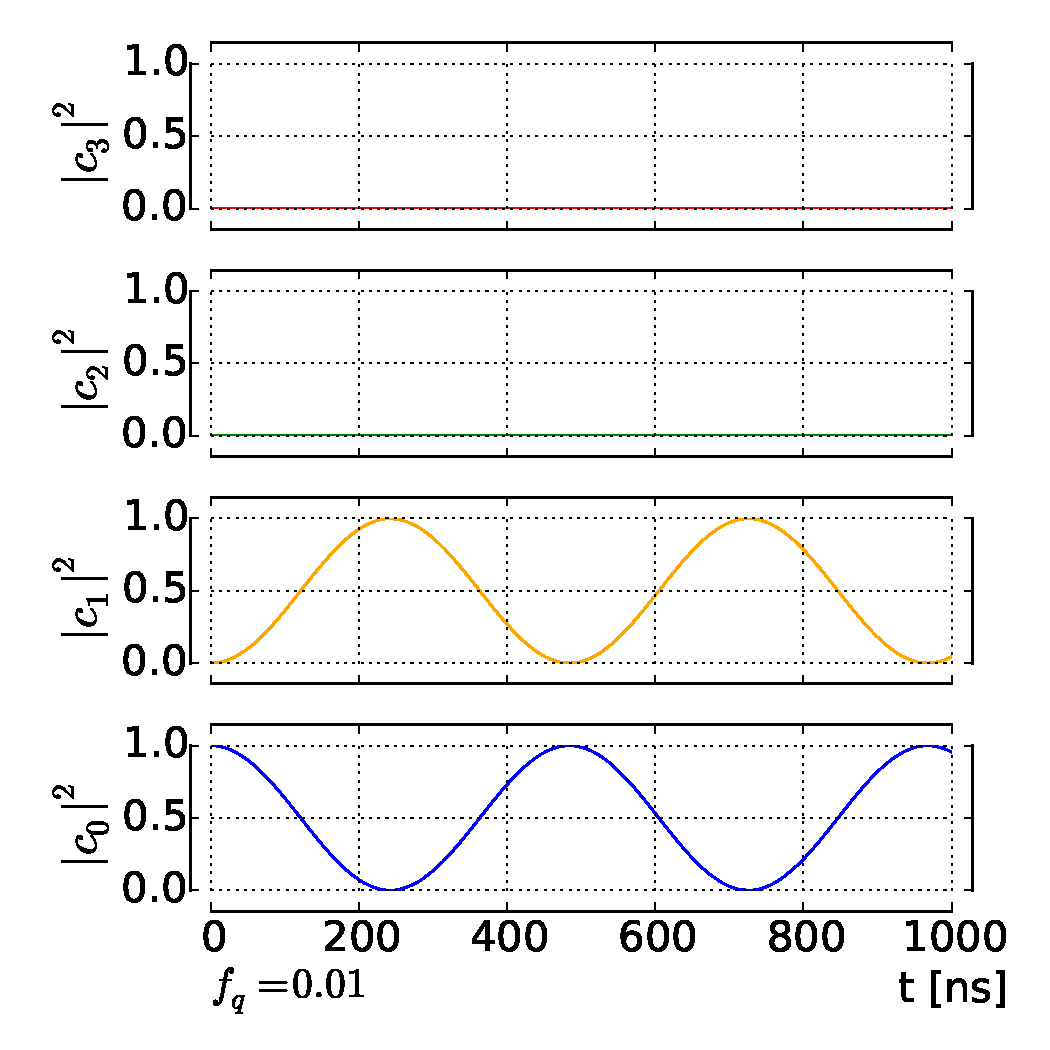
\includegraphics[width=\textwidth]{tr_weak_dr}
\end{subfigure}
\begin{subfigure}[t]{0.45\textwidth}
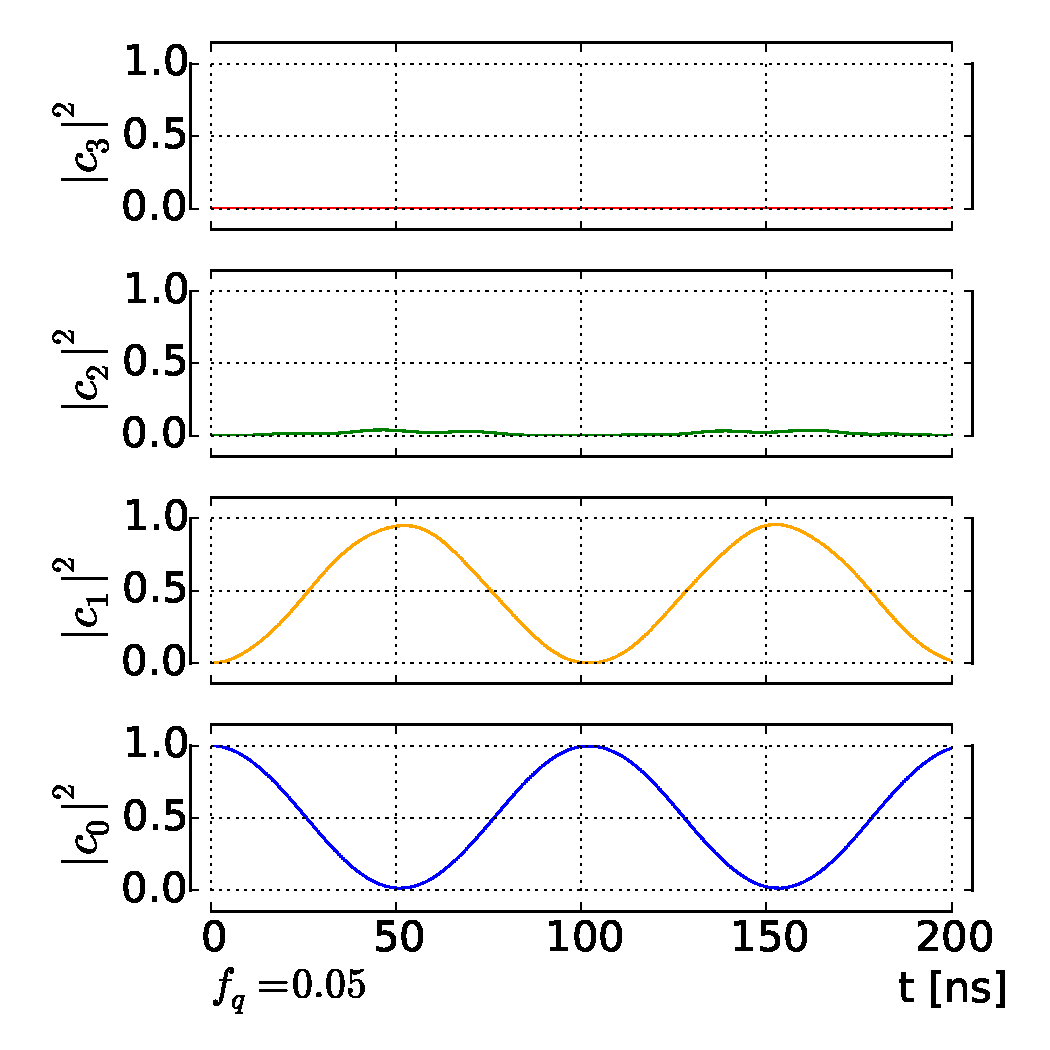
\includegraphics[width=\textwidth]{tr_int_dr}
\end{subfigure}

\begin{subfigure}[t]{0.45\textwidth}
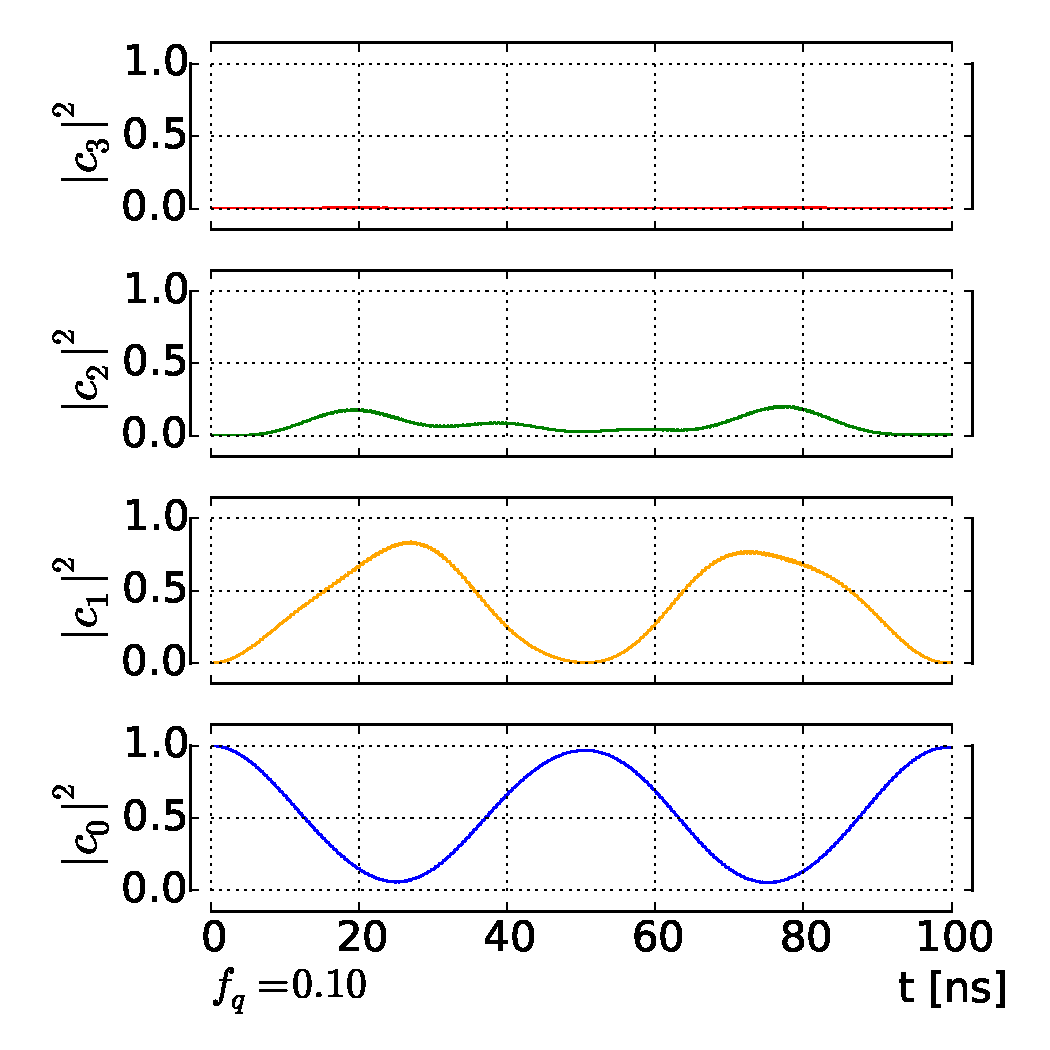
\includegraphics[width=\textwidth]{tr_str_dr}
\end{subfigure}
\begin{subfigure}[t]{0.45\textwidth}
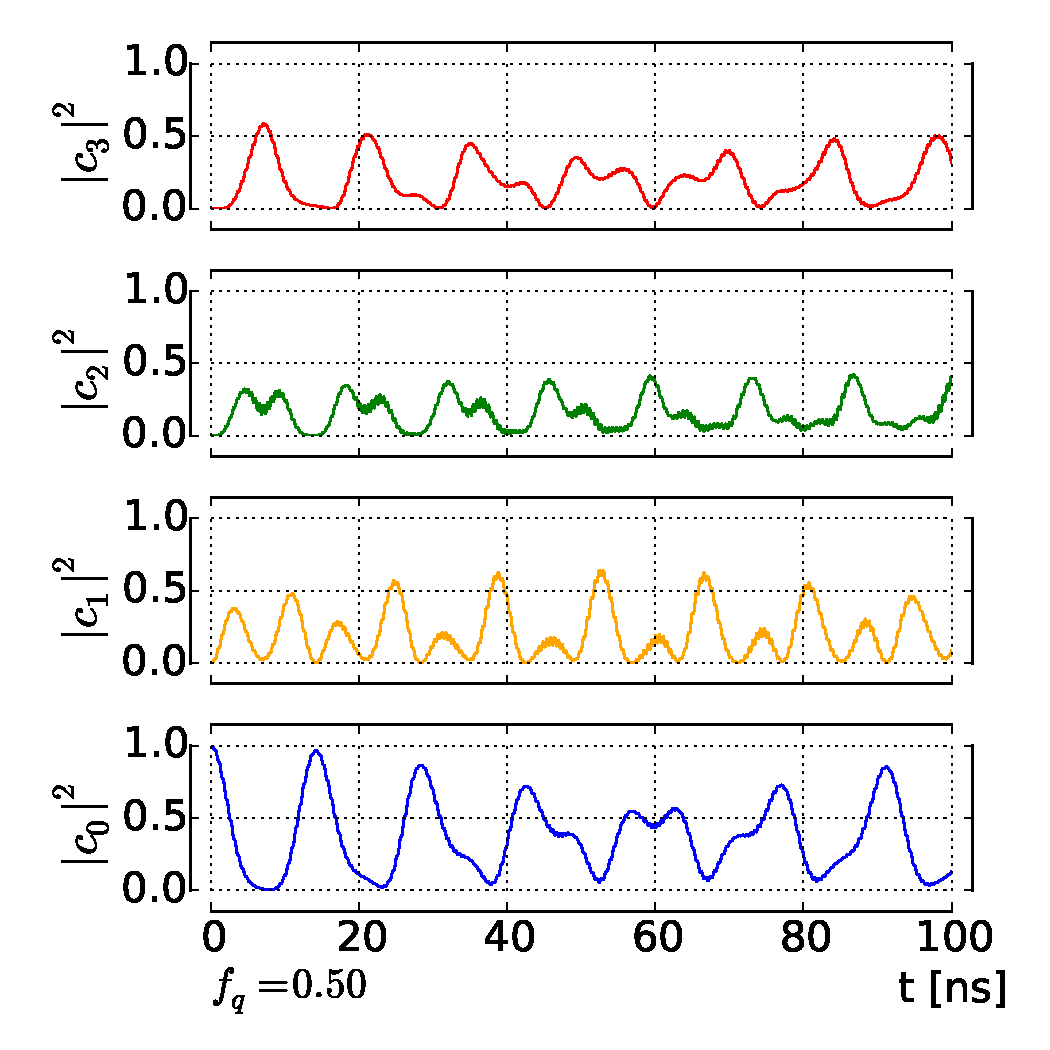
\includegraphics[width=\textwidth]{tr_vstr_dr}
\end{subfigure}
\caption{Dynamics of the isolated driven transmon qubit with different drive strengths $f_q$ = 0.01-0.5 rad/ns, where $f_q$ is an effective amplitude of the drive \eqref{eq:driving_q} $f_q (t) = f_q \sin(\omega_{01} t)$. It can be seen that significant distortions and leakage to higher levels occur when amplitude is too large.}
\label{fig:driven_tr}
\end{figure}

\subsection{Relaxation dynamics (driven and undriven)}

The relaxation process for the transmon is simulated using a Lindbladian master equation with a following dissipative operator:
\begin{equation}
\hat c = \sum_{j\geq 0}^\infty \frac{n_{j\,j+1} }{n_{01}}\ket{j}\bra{j+1}
\end{equation}
which is, obviously, from the definition is a lowering operator. It becomes the destruction operator of the standard harmonic oscillator in the limit of very large $E_J/E_C$, so it's a good operator use for  modelling of the relaxation channel. For a deeper review on this see L.S. Bishop's thesis.\cite{Bishop2010}

The dynamics of the dissipative transmon then will be governed by the following equation:
\begin{equation}
\frac{\partial}{\partial t} \hat{\rho}_q = \frac{i}{\hbar}[\hat{\rho}_q, \hat{\mathcal{H}}_q+\hat{\mathcal{H}}_q^d(t)] + \gamma \mathcal{D}[\hat c]\hat\rho_q,
\label{eq:tr_dissip_dyn}
\end{equation}
where $ \mathcal{D}[\hat{\mathcal{O}}]\hat\rho_q = \hat{\mathcal{O}} \hat\rho_q \hat{\mathcal{O}}^\dag - \frac{1}{2}\{\hat{\mathcal{O}}^\dag \hat{\mathcal{O}}, \hat\rho_q \}$ and $\gamma$ is the relaxation rate. Dephasing may also be added in a similar way.

Below the dynamics of the undriven relaxation and excitation with strong driving are presented as examples of the solution of \eqref{eq:tr_dissip_dyn}.

\begin{figure}[h]
\includegraphics[width=.5\textwidth]{tr_decay}\hspace{-7.5cm}\textbf{(a)}\hspace{6.5cm}
\includegraphics[width=.5\textwidth]{tr_str_dr_decay}\hspace{-7.5cm}\textbf{(b)}\hspace{6.5cm}
\caption{Behaviour of the equation \eqref{eq:tr_dissip_dyn}, represented as populations of the eigenstates depending on time. \textbf{(a)} Relaxation of the first excited state without any driving. The population reaches $1/e$ in $1/\gamma$ ns, as expected. \textbf{(b)} Excitation of the ground state into the steady state which is an incoherent mixture of the first three states. Driving is resonant with $ge$ transition of the transmon.}
\end{figure}

\subsection{Linewidth dependence on drive power} \label{subsec:linewidth}

Knowing the way to model the relaxation of the qubit it's possible to compare the relaxation rate with the linewidth of the qubit on the population graph. The way is to simulate the evolution until the steady state is reached for all driving frequencies around the resonance, calculate populations of the excited state for each reached steady state and then measure the width at the half-maximum of the resulting peak. However, for two-level dynamics the linewidth $\delta \omega$ depends on the driving power as the Rabi oscillations are induced between the levels. So for correct determination of the linewidth it's necessary to measure the linewidth at low driving amplitudes.

Before demonstrating the numerical results for the transmon qubit, a brief analytical solution for the problem in the case of a two-level system will be shown. The master equation for this problem is as follows (within RWA):
\[
\frac{\partial}{\partial t} \hat{\rho}_{tls} = \frac{i}{\hbar}[\hat{\rho}_{tls}, \frac{\hbar (\overbrace{\omega_{tls}-\omega_d}^{\Delta\omega})}{2} \hat{\sigma}_z+\frac{\hbar \Omega_R}{2} \hat{\sigma}_x] + \gamma \mathcal{D}[\hat \sigma^-]\hat\rho_{tls}.
\]
Knowing that $\text{Tr}[\hat\rho_{tls}]=1$ and that $\hat\rho_{tls}=\hat\rho_{tls}^\dag$ we can write down three ODEs from this master equation:
\[
\begin{gathered}
\frac{d}{d t} {ρ_{11}}{\left (t \right )} = - γ {ρ_{11}}{\left (t \right )} + i \left(\frac{Ω_{R}}{2} {ρ_{12}}{\left (t \right )} - \frac{Ω_{R}}{2} {ρ_{21}}{\left (t \right )}\right), \\
\frac{d}{d t} {ρ_{12}}{\left (t \right )} = - \frac{γ}{2} {ρ_{12}}{\left (t \right )} + i \left( \frac{Ω_{R}}{2} {ρ_{11}}{\left (t \right )} - \frac{Ω_{R}}{2} \left(1- {ρ_{11}}{\left (t \right )} \right) - \Delta ω {ρ_{12}}{\left (t \right )}\right),\\
{ρ_{21}}{\left (t \right )} = {ρ_{12}}^\dag{\left (t \right )}.
\end{gathered}
\]

It is practical for our case to solve these equations for steady state, when $\frac{\partial}{\partial t} \hat{\rho}_{tls} = 0$. The matrix elements then are
\[
ρ_{11} = \frac{Ω_{R}^{2}}{2 Ω_{R}^{2} + γ^{2} + 4 \Delta ω^{2}},\quad
ρ_{12} = - \frac{Ω_{R} \left(i γ + 2 \Delta ω\right)}{2 Ω_{R}^{2} + γ^{2} + 4 \Delta ω^{2}},\quad
ρ_{21} = \frac{Ω_{R} \left(i γ - 2 \Delta ω\right)}{2 Ω_{R}^{2} + γ^{2} + 4 \Delta ω^{2}}.
\]

From here it is easy to find the analytical linewidth at half maximum of the $\rho_{11}(\omega_d)$:
\[
\delta\omega = \sqrt{2\Omega_R^2+\gamma^2}.
\]

When the $\Omega_R \rightarrow 0,\ \delta\omega\rightarrow\gamma$, and thus it is possible to extract $T_1$ in case of absence of pure dephasing or at least to put a lower bound on it if the pure dephasing is present. It is important to notice that in the experiment the measured frequency is expressed in Hz though $\delta\omega$ is in rad/s. Therefore, the experimental linewidth should be, firstly, measured at very low powers and, secondly, multiplied by $2\pi$ to obtain $\gamma$. In the presence of pure dephasing the formula for $\delta\omega$ becomes a bit more complicated, but also can be straightforwardly calculated with use of Computer Algebra Systems:
\[
\delta\omega_{\text{with dephasing}} = \sqrt{2Ω_{R}^{2} (1+2 γ_{ϕ}/\gamma) + (\gamma +2\gamma_\phi)^2} \xrightarrow[\Omega_R\rightarrow 0]{} γ + 2γ_{ϕ}.
\]


\begin{figure}[h!]
\centering
\includegraphics[width=\textwidth]{transmon_transtitions}

\includegraphics[width=\textwidth]{transmon_transtitions_narroww_gamma5e-3}

\includegraphics[width=0.7\textwidth]{linewidth_prop_ss}

\caption{Linewidth analysis in dependence on the driving power $f_q$ for $\gamma = 5$ rad/$\mu$s. As can be seen, with the increasing drive amplitude the spectral line becomes wider. In contrast, its width levels off when the amplitude is decreased, and reaches asymptotically the value of $\frac{\gamma}{2\pi}$. The factor $2\pi$ appears as the linewidth found in the experiment usually is in Hz, but the equality that holds is that $\gamma = \delta\omega$, and $\delta\omega = 2\pi\delta\nu$.}
\label{fig:transmon_lw}
\end{figure}  

Interestingly enough, if there's no relaxation and $\gamma = 0$, the formula shows divergence of the linewidth. This happens because the solution of the master equation in this case yields $\rho_{11} = 1/2$ in the steady state, independent of the driving detuning and driving strength, and thus the linewidth can't at all be defined.

For the transmon the two-level dynamics between its ground and first excited state is equivalent; however, there's no simple analytical solution for the dynamics. To see the behaviour is same in this case we have to resort to numerical modelling (see \autoref{fig:transmon_lw}).
As can be seen, the linewidth $\delta\omega$ grows with the increased power, and, in contrast, saturates at low powers, reaching the value of $\gamma$.

\chapter{Experimental methods}

\section{Experimental setup and equipment}


\begin{figure}[h!]
\centering
\includegraphics[width=\textwidth]{BF_for_albmstu1}
\caption{Example configuration of the 15 mK stage of the BF LD 250 fridge in the RQC lab at ISSP with three samples installed (with false colors added). \textbf{(a)} Front-bottom view of the 25 mK flange. Cyan color highlights the cylindric cryoperm shield inside which the sample holder resides. \textbf{(b)} Back view, violet color shows the circulators with  a thick copper wire wrapped around them for thermalization. \textbf{(c)} Front-top view, where the 2-channel  microwave switch is shown (magenta) and the hybrid coupler (blue, left in true color) used to measure several samples using only one low-noise HEMT amplifier. \textbf{(d)} Side view, the two unshielded sample holders similar to the one concealed under the shield from (a) are shown in yellow.}
\label{fig:configuratio_photo}
\end{figure}

\begin{figure}[h!]
\centering
\includegraphics[width=.8\textwidth]{setup}
\caption{Schematic of the example configuration shown in \autoref{fig:configuratio_photo}.}
\end{figure}

\section{Two-tone spectroscopy}
\label{sec:2tone}

This type of measurement is conducted with an additional microwave tone from the microwave source, which induced the transitions from ground state of the system to higher levels and transition frequencies from there then are being probed by the VNA. Practically this is realized by setting the VNA to measure single point at the shifted resonator  frequency $\omega_r + \chi_0$ (see \autoref{fig:diagram}). This results in a low transmission as photons get absorbed by the system. Then the qubit is biased, and the frequency on the $\mu$-wave source is swept through some values at each given bias. When the frequency of the latter coincides with some allowed transition frequency of the system at given bias, the system leaves its ground state, and the VNA is not probing a correct transition frequency any more. For example, if second tone has induced qubit $ge$ transition, the correct resonator frequency would be $\omega_r + \chi_1$ and the lowest transmission will be observed there (see \autoref{fig:diagram} again). Thus, at $\omega_r + \chi_0$ where the VNA is measuring the transmission would become higher than it was when the second tone missed the $ge$ transition. 

In reality the situation is a bit more complicated as long as constant microwave tone induces Rabi oscillations between levels if it is resonant with the corresponding transition and after all the VNA will be probing transitions from an incoherent mixture of states (i.e. $\hat \rho = \frac{1}{2} [\ket{0, g}\bra{0,g} + \ket{0, e}\bra{0,e}]$) which depends on the drive strength; however, the transmission still ends up being higher when the second tone induces transitions from ground state. All said above can be applied also to the transmission phase, however the phase at resonance will become either higher of lower depending on the direction of the resonance shift as long as the phase behaves linearly around the resonance. It is thus much more sensitive when the width of the resonance peak is larger than the dispersive shift. 

It is possible to easily extract the linewidth of the qubit which was described in Section \ref{subsec:linewidth} if the resonator linewidth is larger than the dispersive shift. This can be done by setting the VNA frequency to the point of smallest transmission and studying the phase data. The phase will be a linear function of the frequency near this point, and the frequency, in its turn, will be a linear function of the population of the excited state. This means that the width at the half maximum of the 2-tone peak will be same as the width of the peak of the population. If, in contrast, the resonator linewidth is smaller than the dispersive shift, it would be necessary to extract the frequency of the resonator for each point and then plot it against the 2$^{\text{nd}}$ tone frequency to preserve the linearity and measure the linewidth correctly.

This method works well in the dispersive limit when the qubit-resonator detuning $\Delta_\omega = \omega_r - \omega_{ge}$ is large compared to the coupling strength $g$.

\chapter{Experimental results}

\section{Proof-of-concept design}

\subsection{Geometry and parameters}

The first sample that was measured was created from a proof-of-concept design, which was aimed at testing general properties of the simplest Xmon-based cQED systems. The easiest way to gain insight about the structure of the sample is to look at \autoref{fig:first_chip_design_full} where some of the main parts of its design are shown. The chip is 8 mm long and 4 mm wide and consists basically of six isolated qubit-resonator systems. 

All of the resonators were $\lambda/4$ with frequencies designed to be $6, 6.5, 6.9,7,7.1,8$ GHz for devices I-VI, respectively. Their coplanar parameters are $7\,\mu$m for the central wire width and $4\,\mu$m for the gaps.

The qubits were designed to be identical, with $C_\Sigma \approx 80$ fF and $I_{C, \Sigma} = 60$ nA, giving the $\omega_{01}/2\pi \approx 7$ GHz at their flux sweet-spot ($\Phi_{ext}=0$) and anharmonicity of approximately $-230$ MHz.

Two test structures at the sides of the chip were also included to allow direct DC measurement of the SQUIDs created during the shadow evaporation.

\subsection{Purposes and implementation}

The main targets for the chip were:
\begin{enumerate}[label=(\alph*), leftmargin=1.5cm]
\itemsep0pt
 \item to check the measurement setup
 \item to check the calculations for the frequencies and the coupling strengths
 \item to roughly check the coherence of Xmons
 \item to estimate the reproducibility of the junctions 
 \item to observe the AC-Stark shift 
 \item to observe high-power multiphoton transitions and sidebands
 \item to check for the interesting effects caused by different resonator detunings at sweet-spot  
\end{enumerate}

\begin{figure}[h!]
\centering
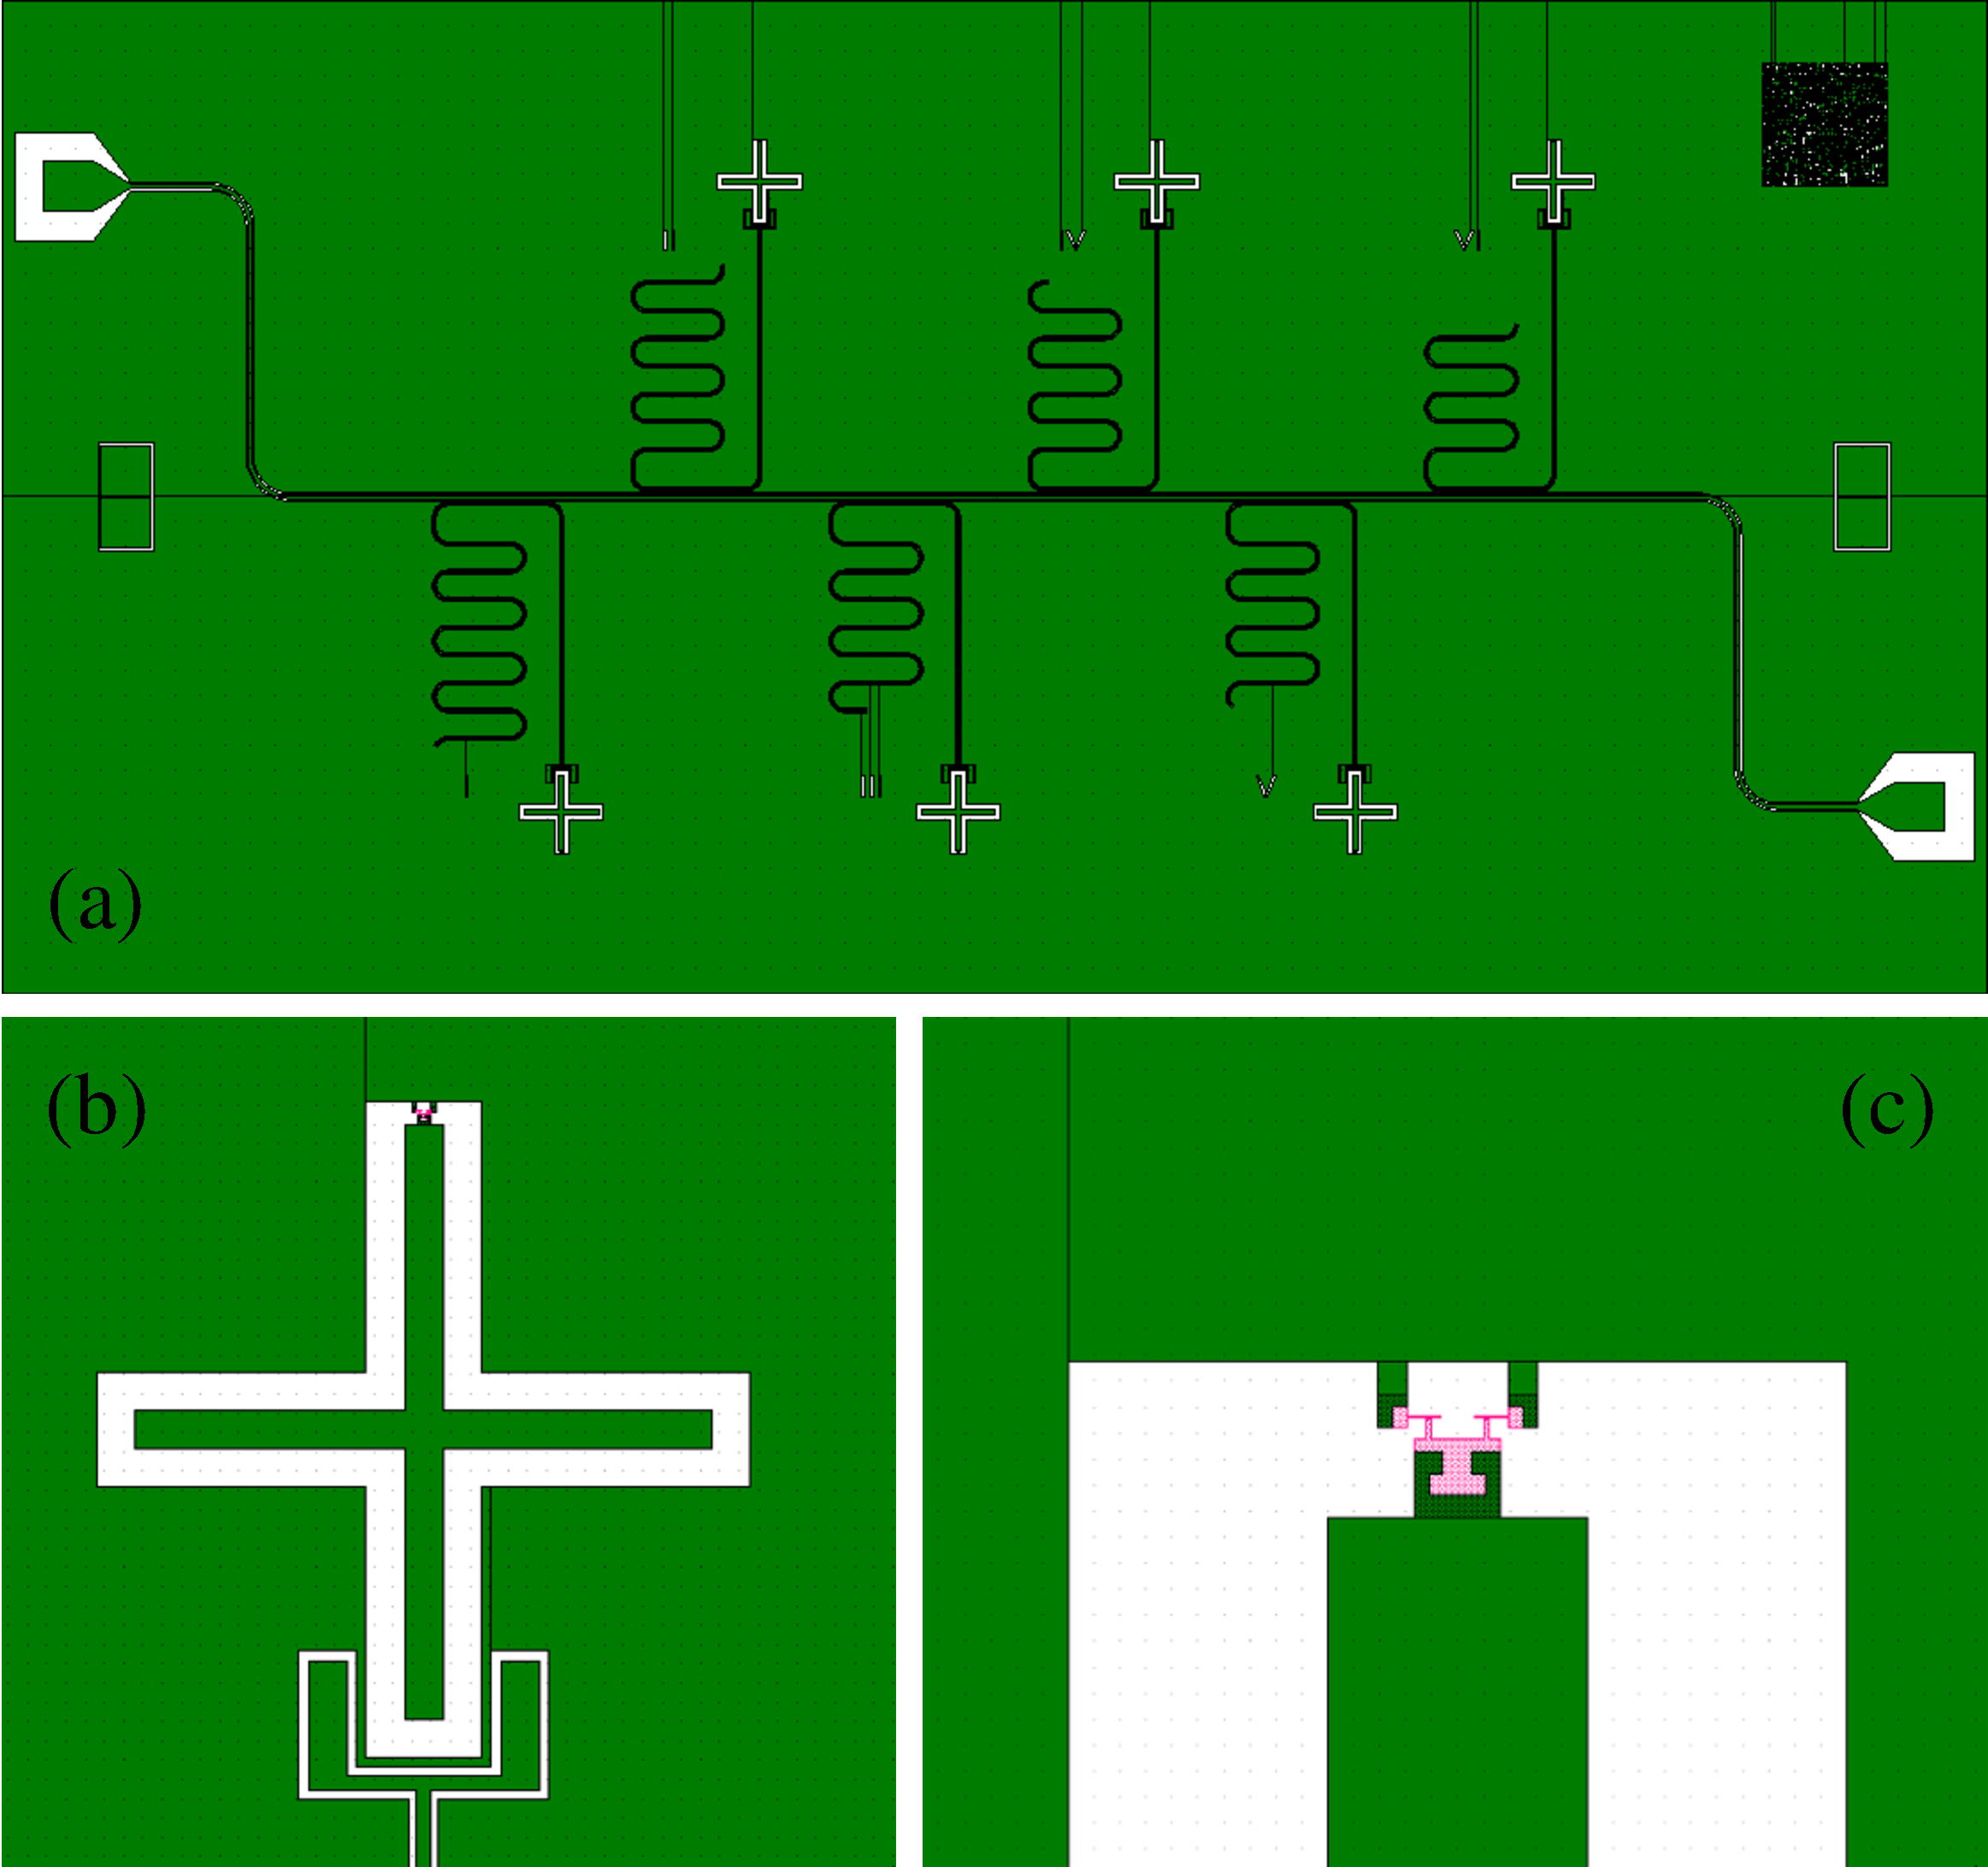
\includegraphics[width=0.9\textwidth]{chip_design_full}
\caption{\textbf{(a)} Large-scale image of the design used for the proof-of-concept sample. The chip (8x4 mm) consists of six $\lambda/4$ CPW resonators coupled capacitively to the feedline each with an Xmon qubit at the open end. \textbf{(b)} Zoomed area around one of the qubits, showing its cross-shaped capacitor and the ``claw'' coupler of its resonator. \textbf{(c)} Zoom around one of the qubits' SQUIDs. Pink areas denote the e-beam mask that was used for shadow evaporation.}
\label{fig:first_chip_design_full}
\end{figure}

The sample was fabricated in the cleanroom facility at MIPT, in a two-step process. Firstly, electron beam lithography was used to form the shadow evaporation mask for the pads with junctions and Al was shadow evaporated on the Plassys unit ($\pm 7^\circ$). Secondly, the photolithograpy was used to pattern larger structures like the feedline, resonators and Xmons' capacitors aligned with e-beam lithography and finally another layer of Al was deposited.	

\begin{figure}
\centering
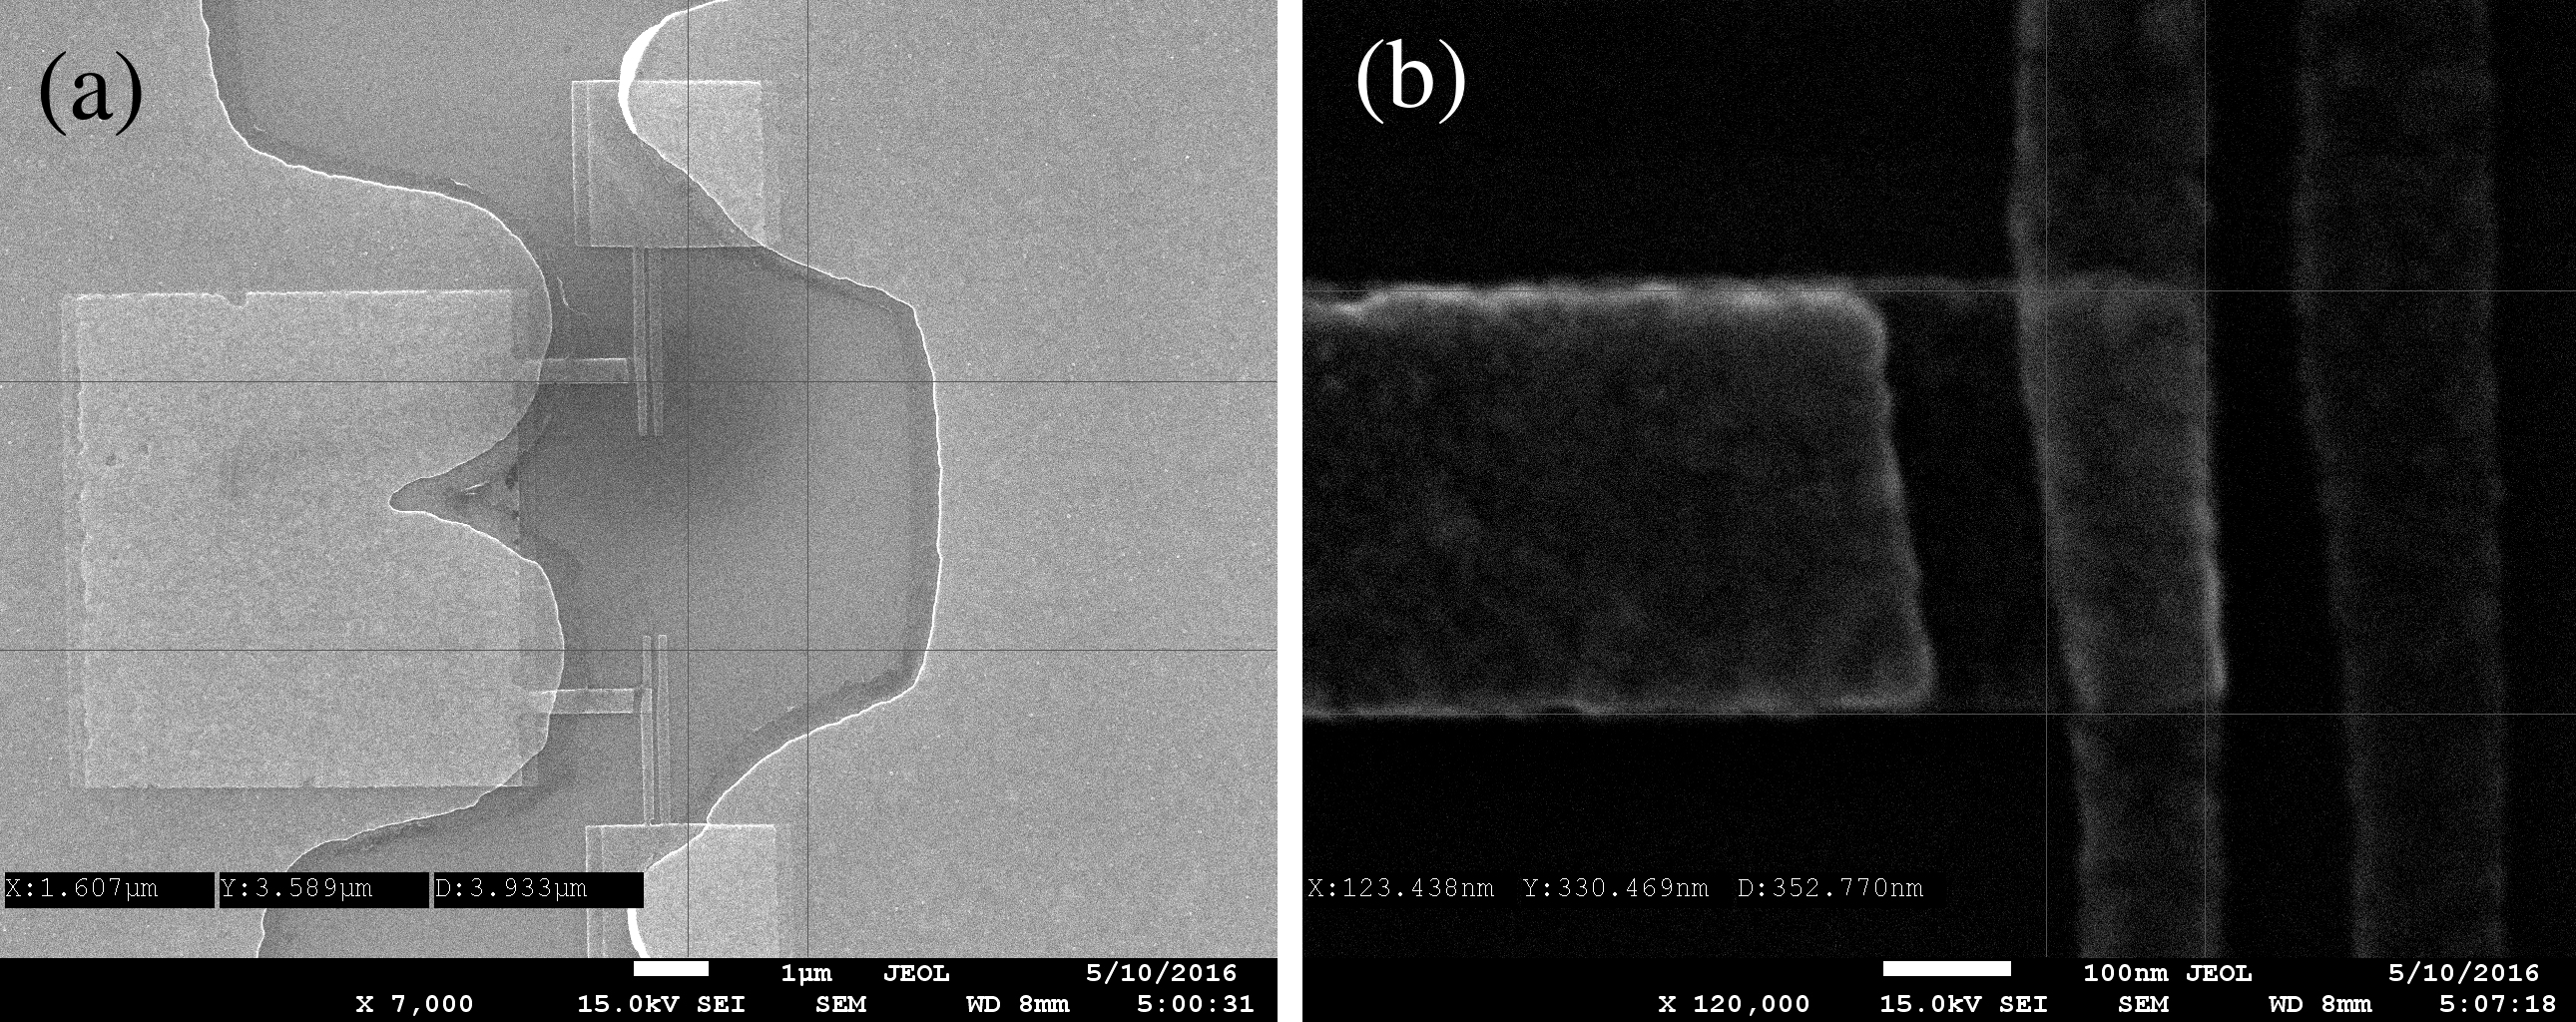
\includegraphics[width=0.9\textwidth]{X_mon_JJ_SQUID}
\caption{\textbf{(a)} SEM micrograph of the SQUID of one of the test structures on the chip. One can see that photo- and electron lithography are aligned, however fine structures \autoref{fig:first_chip_design_full}~(c) were not resolved during the second step. \textbf{(b)} Enlarged view on one of the junctions (upper). Its area is approximately $120\times 330\approx 0.4\, \mu m^2$, in the design it's $0.3\,\mu m^2$.} 
\end{figure}

\subsection{Measurement setup}

The sample was measured at ISSP in laboratory of RQC. Cryogenic equipment was represented by BlueFors LD250 dilution refrigerator, with base temperature of 16 mK. The microwave equipment included R\&S ZNB 10 kHz-20 GHz vector network analyser,  Agilent E8257D 100 kHz - 40 GHz analog signal generator. The sample was flux biased using Keithley 6221 current source.

Microwave line was thermalized with 60 dB of attenuation, additional 20 dB of attenuation were introduced on a directional coupler which added the second tone from the $\mu$-wave source. After leaving the sample the signal passed through two isolators and a hybrid coupler, which was used before to measure two samples during single cooldown. Finally, the signal was amplified with 4-8 GHz LNF amplifier at 4 K and a with a room-temperature amplifier.

The sample holder that was used was designed for 10x10 mm chips, so the bondwires had a relatively large length of 1 mm which of course deteriorated the overall transmission. Chip lay directly on the copper disk of the bottom part of the sample holder with no hole carved under it. Around the sample holder a superconducting coil was wound which has been supplied using the current source mentioned above.

The magnetic shielding of the sample holder was achieved via a cryoperm shield. A superconducting shield was not installed in this run due to the lack of space inside the magnetic shield, which may have influenced the noise background.


\subsection{Characterization of the resonators}

As a first step of characterizing the sample a study of the resonances was performed. In \autoref{fig:first_resonators_general} the power transmission through the cryostat is shown. In can be seen that in overall the transmission level is at approximately $-35$ dB. As long as the amplifiers add 60 dB the directional coupler and the hybrid coupler subtract 23 dB, it can be inferred that the sample in the sampleholder itself has approximately -10 dB transmission. This should be improved with better impedance matching to reduce noise. Secondly, there is a clear 300 MHz-wide dip in the transmission around 6.2 GHz, which should also be eliminated.

\begin{figure}[h]
\centering
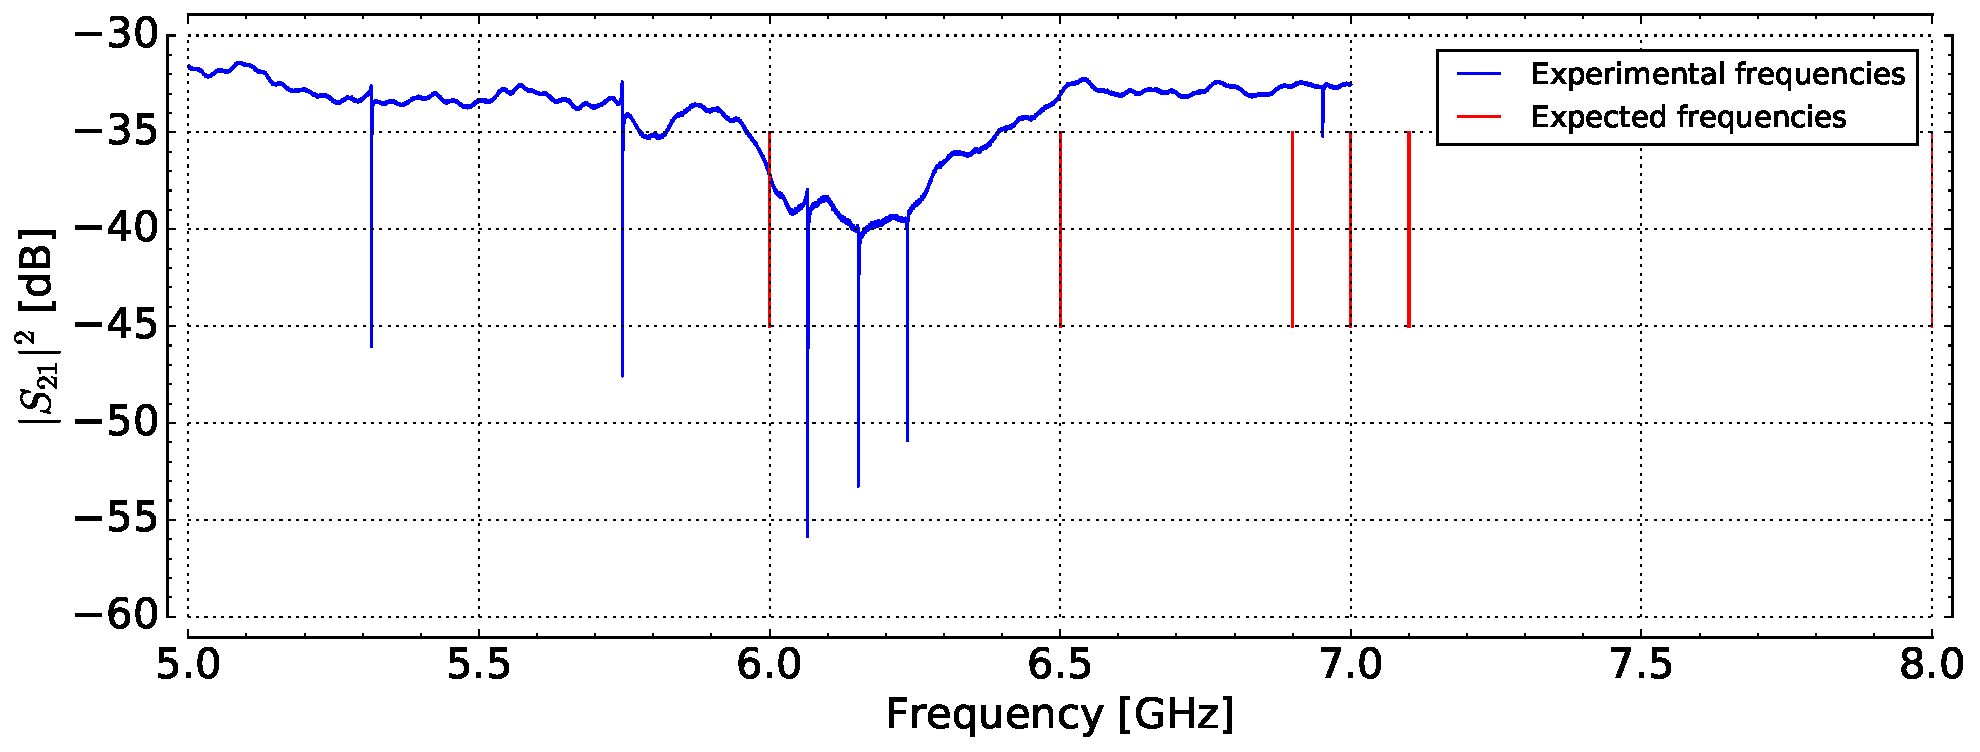
\includegraphics[width=\textwidth]{xmon-first-try_general15x5}
\caption{General view of the resonances. All six resonances are visible, however shifted far down in frequency. This shift is due to a mistake in the design which didn't compensate for the ``claw'' couplers at the resonator ends.}
\label{fig:first_resonators_general}
\end{figure}

All resonators are functional which can be seen from the presence of six sharp dips in transmission. The frequencies at which the dips occur are significantly lower than expected because there was a flaw in the macro code which draws the design. The frequency compensation routine made specifically to calculate the frequency shift\cite{Sank2014} caused by the ``claw'' coupler at the end of the resonator was not executed, so the length of the resonators became larger than it should have been. At higher frequencies the phase shift of the ``claw'' is larger so the frequency discord is larger there.

Below the results obtained using the \textit{circlefit}\cite{probst2015} fitting method are presented. Each peak from \autoref{fig:first_resonators_general} was enlarged and scanned with a fine resolution and averaged to reduce noise (more averages on low and less on high powers). Then for each power complex $S_{21}$ data for each scan area around a resonance was recorded.

After all of the data had been obtained, the fitting procedure has been applied for every scan at each power. The full fitting process is described in depth in the original publication\cite{probst2015}. In practice the whole algorithm is encapsulated in several function calls of the library called \textit{resonator tools} that the authors have kindly provided via \href{https://github.com/sebastianprobst/resonatortools}{GitHub}. Fitting results are summarized in \autoref{fig:first_q_factors}.

\begin{figure}[t]
\centering
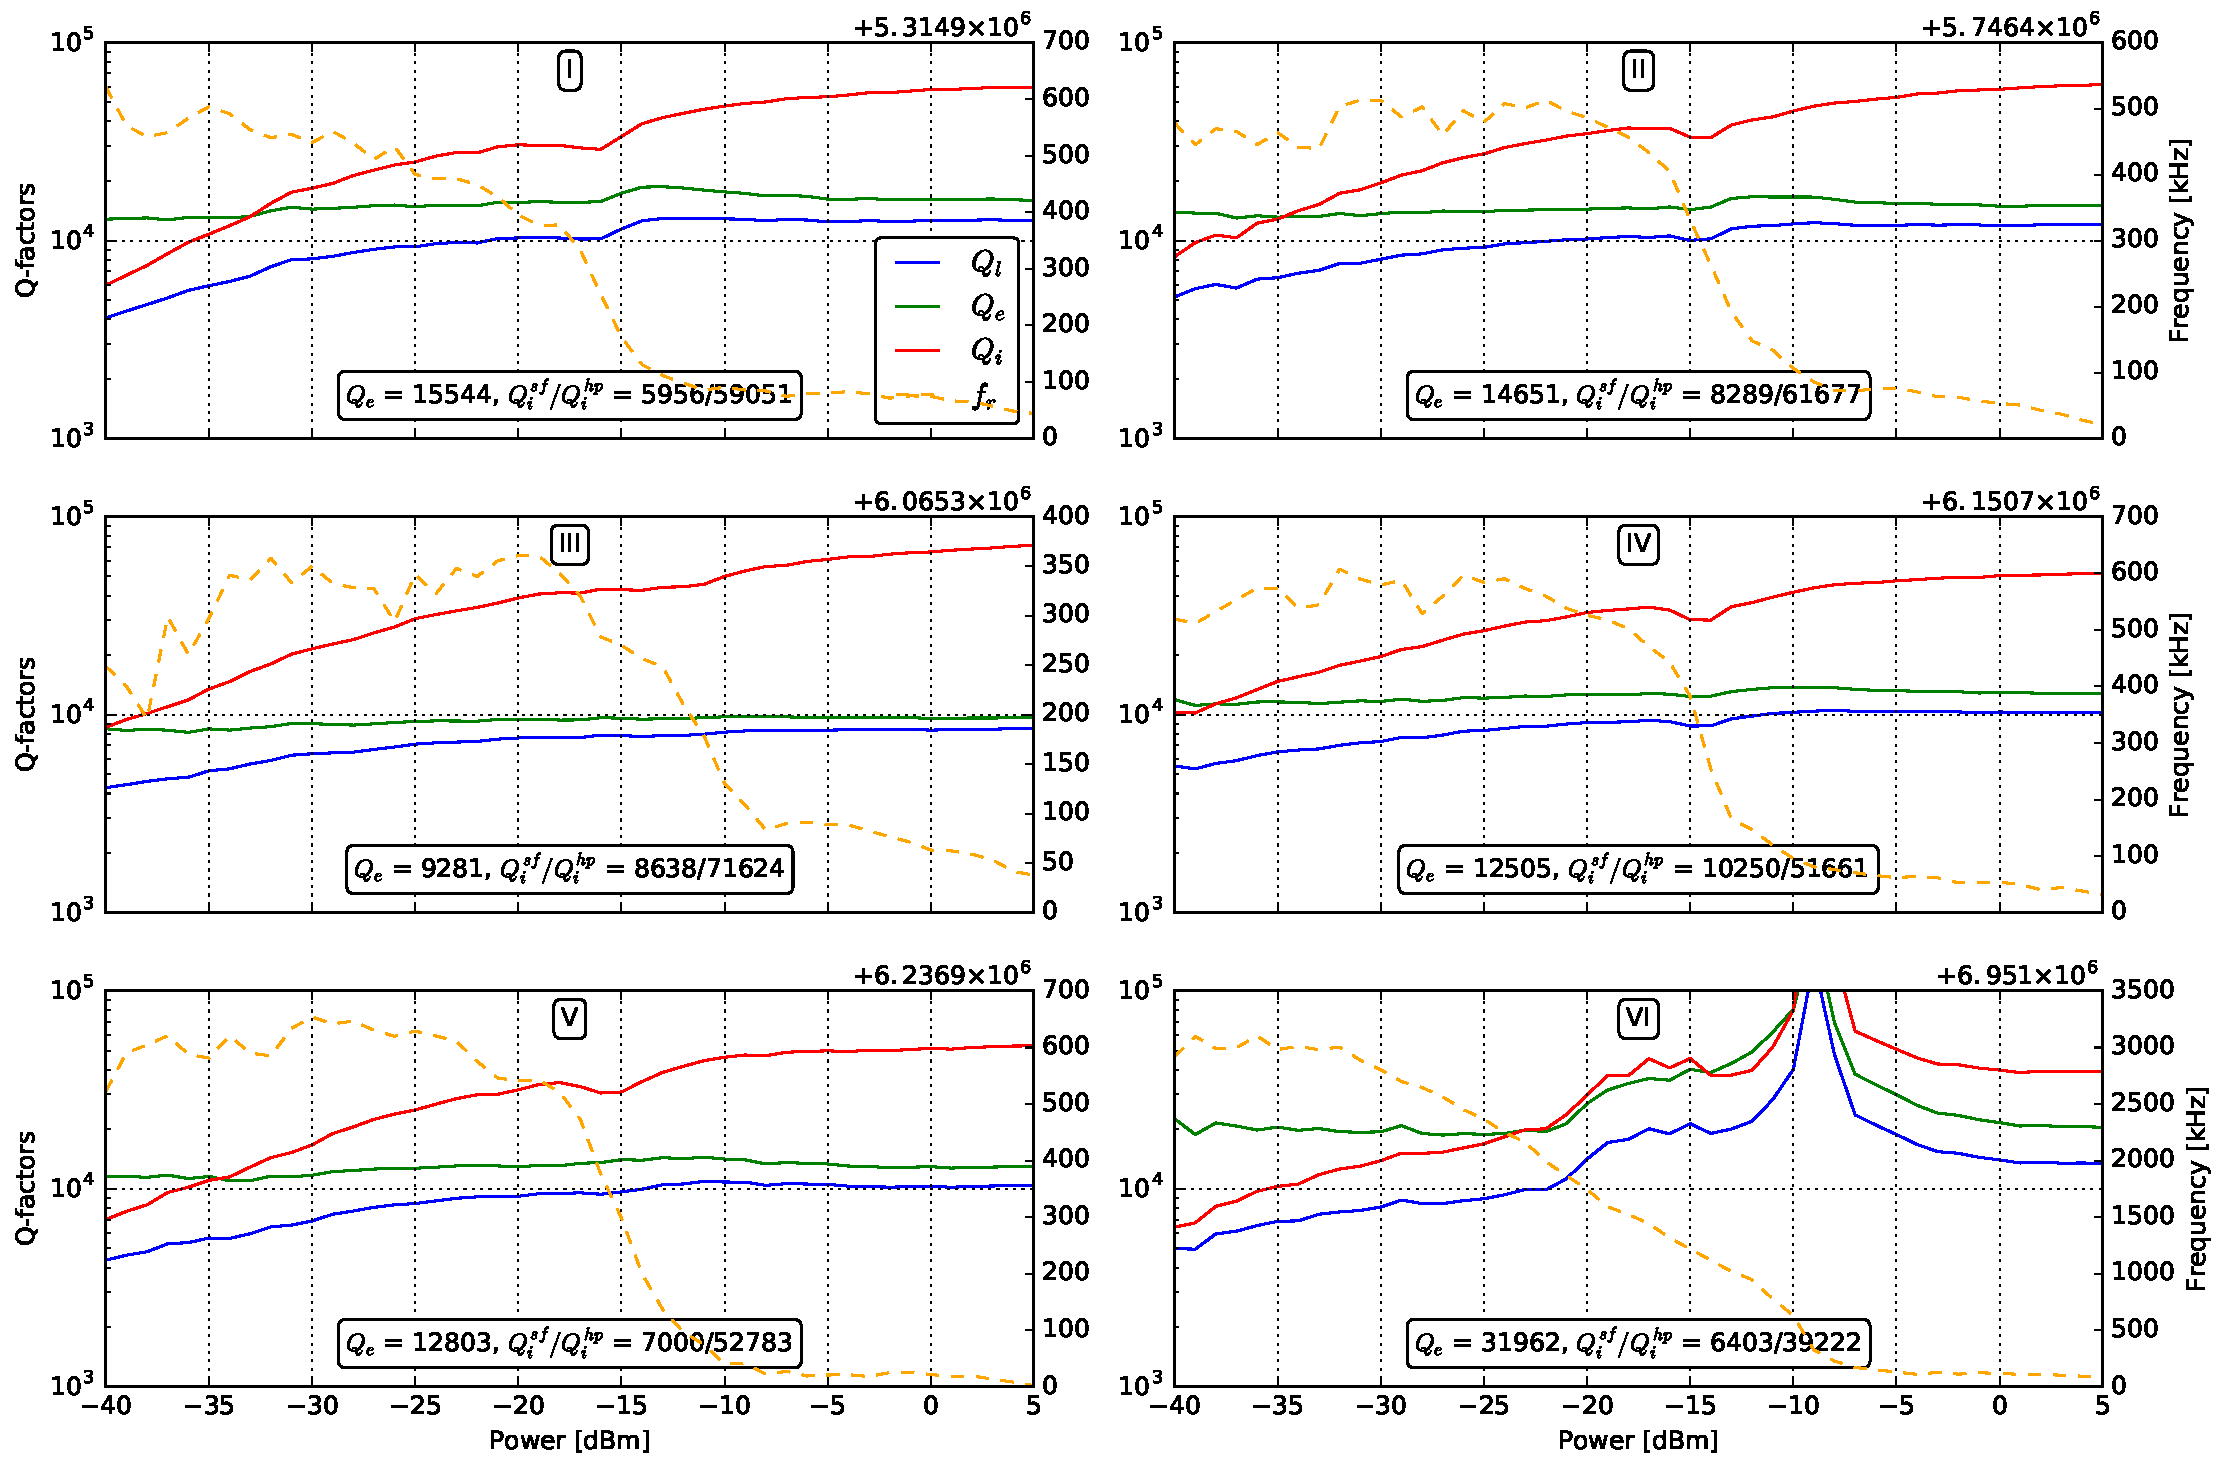
\includegraphics[width=\textwidth]{q-factors-and-freqs_xmon_first_try}
\caption{Various quality factors and frequencies depending on radiation power. Single photon limit is near -40 dBm on the VNA summed with 80 dB of attenuation, saturation limit near 5 dBm on the VNA. All devices show standard behaviour except for the VI\textsuperscript{th} which loses its shape and cannot be fit correctly at powers above -20 dBm.}
\label{fig:first_q_factors}
\end{figure}

It is well-known\cite{wang2009} that for superconducting microwave resonators the internal quality factor experiences an increase in value when probed with higher power. This effect is believed to occur due to the presence of two-level defects or two-level systems (TLS) with a dipole moment in the areas of high electric fields which resonator creates. As long as TLSs have same frequency as the measured resonator and coupled strong enough, they will drain excitations from the resonator. However TLSs can only accommodate only one photon at a time; thus, at high probe powers they saturate and do no more participate in resonator relaxation. Therefore, an increase of the internal Q-factor is observed when the resonator is driven with strong microwave fields.

When the resonator is coupled to a weakly nonlinear quantum system like transmon its quality factor will depend strongly on the coherence time of the qubit when their frequencies are close (thus on the flux bias). Therefore, possibly the low (usual $Q_i$ values for similar Al devices are around 3$\cdot 10^4$) internal quality factor values of the resonators at single-photon level are determined by high dissipation in the qubits that were not detuned far enough in frequency.

\begin{figure}
\centering
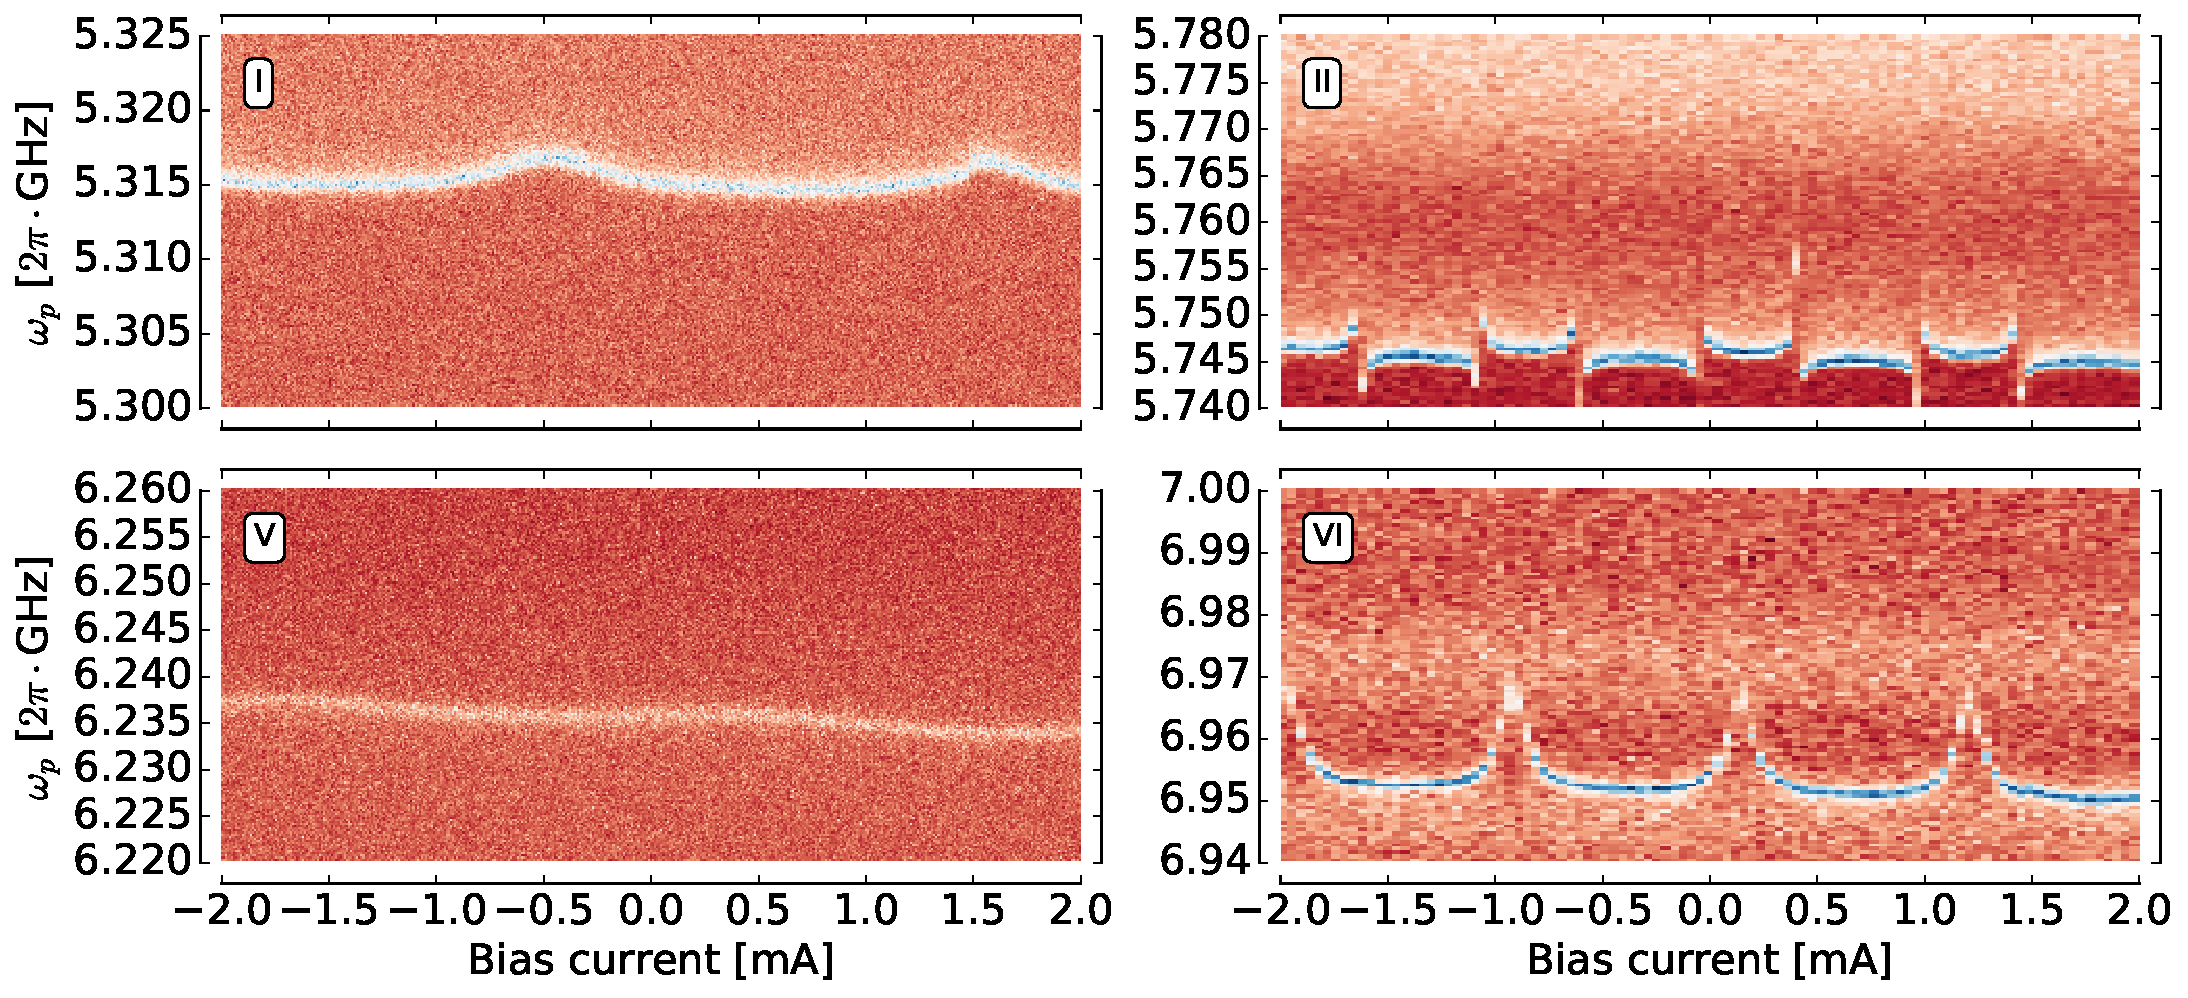
\includegraphics[width=\textwidth]{first_resonators_on_flux}
\caption{Magnetic field influence on frequencies of four devices. Resonators III and IV didn't demonstrate any significant dependence on flux (not shown here).}
\label{fig:first_resonators_on_flux}
\end{figure} 

\subsection{Characterization of the whole cQED systems}

From six systems on the chip only three were studied in detail partly due to lack of time and partly because the overall picture was more or less clear at that point. Firstly the behaviour of the resonators was investigated when the flux bias was being changed. This measurement revealed obvious periodic frequency oscillations in four devices from six, see \autoref{fig:first_resonators_on_flux}. The other two devices didn't show any noticeable periodic flux dependence because one of the qubits (III) had a broken SQUID and the other (IV) probably was much lower in frequency than its resonator.

Firstly system II was measured as long as it has shown the most prominent flux response of all. Then system VI was investigated and, finally, system I. For each of them a two-tone spectroscopy was performed and for II and VI a high-resolution single-tone one as well. Then the data was used to fit the parameters in the model \eqref{eq:hamiltonian} described in \autoref{sec:cQED}. Accordingly, the graphs that are shown below are composed of the experimental spectra overlayed with theoretical curves obtained from numerical solution of the corresponding eigenproblems.

\subsubsection{System II}

\paragraph{Model.} Below all the experimental data will be provided for system II along with theoretical fits of the spectral lines that were observed using the model \eqref{eq:hamiltonian}. Model parameters were fit based on all data on this system and are same for all figures in this section. Before turning to the comparison of the theoretical predictions and experimental results it would be useful to present the model parameters used for fitting which are summarized in \autoref{tab:first_II_params}.

\begin{table}[h]
\centering
\begin{tabular}{l|c}
Parameter & Value \\
\hline 
$C_\kappa$ & 0 fF \\
\hline
$C_g$ & 1.9 fF \\
\hline
$C_q$ & 95 fF \\
\hline
$E_C$ & 200 MHz
\end{tabular}~
\begin{tabular}{l|c}
Parameter & Value\\
\hline
$C_r$ & 444 fF \\
\hline
$L_r$ & 1.72 nH \\
\hline
$I_{C, \Sigma}$ & 69.5 nA \\
\hline
$E_{J, \Sigma}$ & 34.5 GHz
\end{tabular}
\caption{Values of the main parameters defining the spectrum of the model \eqref{eq:hamiltonian}.}
\label{tab:first_II_params}
\end{table}

From these values it's possible to calculate the coupling strength $g \approx 19.6$ MHz between the qubit and the resonator, bare qubit frequency of $\omega^{(0)}_{ge}/2\pi = 7.3$ GHz and bare resonator frequency $\omega^{(0)}_r = 5.758$ GHz. In the coupled system these values are shifted strongly, $\omega_{ge}/2\pi = 7.23$ GHz and $\omega_r = 5.746$ GHz. These shifts are so large (much greater than what would be predicted by the usual dispersive shifts) because of the large value of the Xmon capacitance. Usually cQED systems are treated in the limit of large $C_r \gg C_q, C_g, C_\kappa$ and in this case factors in the terms $\mathcal{\hat H}_q, \mathcal{\hat H}_r $ from \eqref{eq:hamiltonian} can be reduced to their bare uncoupled values. This means the only difference from the uncoupled case is the term $\mathcal{\hat H}_i$, which defines the shifts from the uncoupled frequencies, which are in this case by definition equal to the dispersive shifts. In the studied case $C_q \approx 0.25\, C_r$ and cannot be neglected; thus, the interacting systems are not the same as before coupling, and only the full model \eqref{eq:hamiltonian} taking account of all capacitances can be used to obtain correct results. Despite that after acquiring the new parameters for the interacting systems from \eqref{eq:hamiltonian} the dispersive shifts may be calculated as usual.

The flux normalization on the x-axis was done using data from \autoref{fig:first_resonators_on_flux}~(II) knowing the fact that $\Phi_0$ should be the period of the pattern and that zero flux point is situated at the center of one of the lower branches.

Below in the description of the figures a bit different notation for the transition frequencies may be used than those which denote the theoretical curves on the legends of the graphs. This is due to the fact that in the presence of coupling the qubit spectrum $\omega_{ge}(\Phi_{ext})$ is shared between transitions $\omega_{01}(\Phi_{ext})$ and $\omega_{02}(\Phi_{ext})$ of the full Hamiltonian, so when we say $\omega_{ge}(\Phi_{ext})$ we imply $\omega_{01}(\Phi_{ext})$ and $\omega_{02}(\Phi_{ext})$ for the cases of $\Delta_\omega > 0 $ and $\Delta_\omega < 0$, respectively.

\begin{figure}
\centering
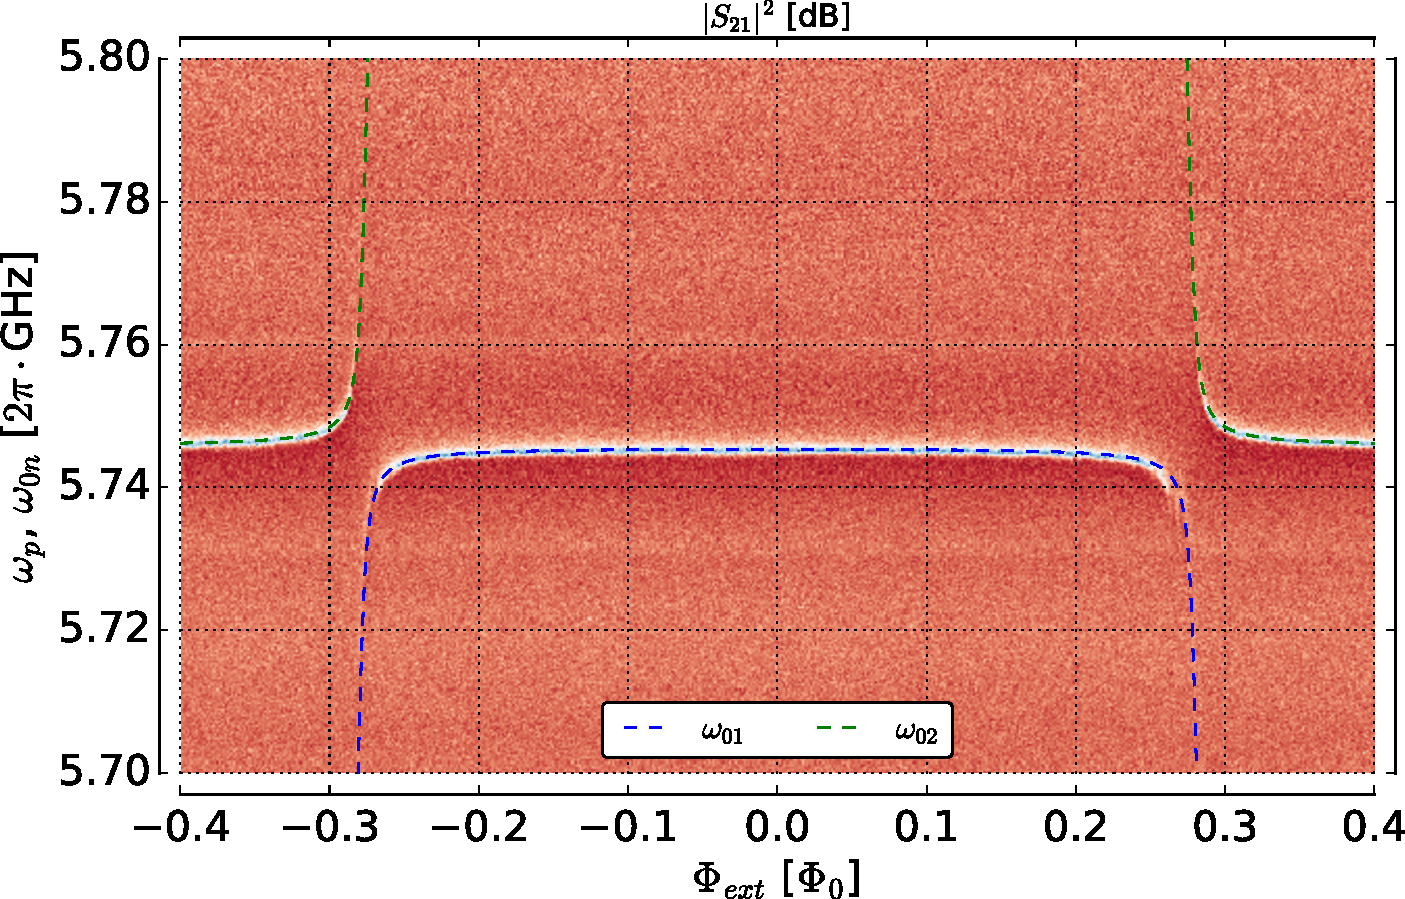
\includegraphics[width=0.9\textwidth]{first_II_anticrossing_fit}
\caption{Anticrossing spectrum of system II with fitting lines obtained by numeric calculation from the model\eqref{eq:hamiltonian} (z-axis normalized). It can be seen that lower branch has some artefacts near the anticrossings which are caused by multiphoton and sideband transitions, signifying that probe power was not at single-photon level. The x-axis is normalized to one flux quantum through the SQUID of the Xmon.}
\label{fig:first_2nd_res_anticrossing}
\end{figure} 

\paragraph{Anticrossing spectrum.} Firstly, a high-resolution scan of one of the anticrossings from \autoref{fig:first_resonators_on_flux}~(II) was obtained. The power level on the VNA was set to -40.0 dBm, which means around -120 dBm at the sample. It is presented in \autoref{fig:first_2nd_res_anticrossing}. It can be seen that a really good agreement between experiment and theory was attained. However there are some discrepancies that can be pointed out: a slight asymmetry of the left and right anticrossings and the reduced brightness of the main branch $\omega_{01}$ on the right. It can be seen clearly from the data that additional multi-photon transitions or sidebands are visible similar to what have been observed before\cite{bishop2009} which indicates that the power was higher than at the single-photon level. Theoretical curves for those transitions were not displayed because the picture becomes too crowded. It is not clear why this effect is stronger in the right anticrossing than in the left one. Further investigation is needed, because at that cooldown due to the setup limitations measurements at lower power were too time consuming because of the low transmission.

\begin{figure}
\centering
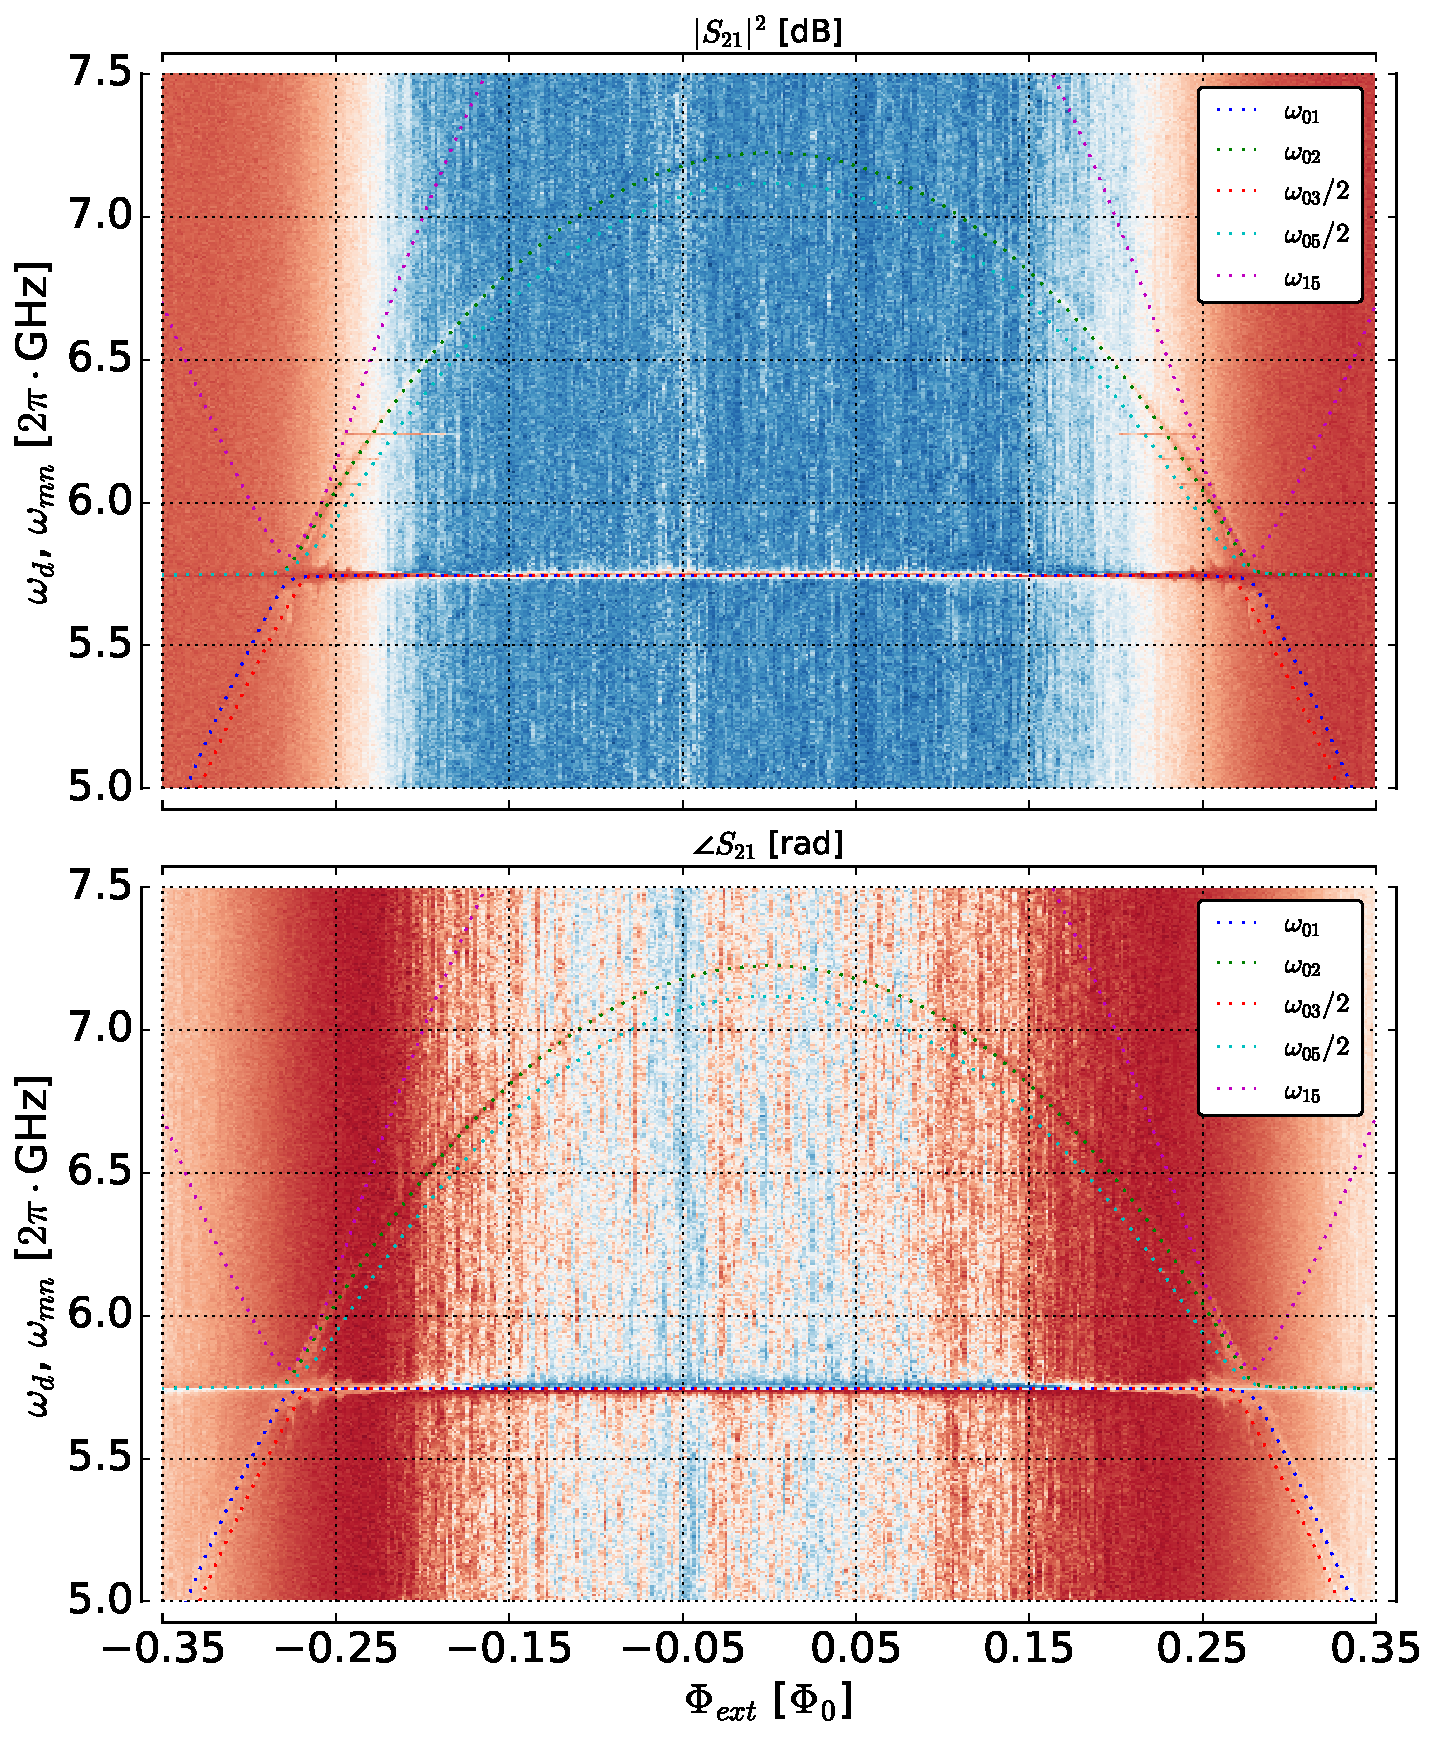
\includegraphics[width=.9\textwidth]{first_II_2tone_fit}
\caption{The two-tone spectrum of system II at -20 dBm power level on the $\mu$-wave source with fitting lines obtained from the model \eqref{eq:hamiltonian}. Various transitions are visible, most pronounced are the horizontal resonator $0n$ transition, the hyperbolic qubit $ge$ transition ($\omega_{01},\ \omega_{02}$) and lower branch of the hyperbolic two-photon $gf$ transition ($\omega_{03}/2$). Also a sideband $\ket{1,g}\rightarrow \ket{0,f}$ is visible ($\omega_{15}$).}
\label{fig:first_II_2tone}
\end{figure}


\paragraph{Two-tone spectroscopy.} Next measurement was a standard two-tone spectroscopy. The results of such measurement at different second tone powers are presented. Firstly, the lowest possible power (-20 dBm) scan was acquired, it is shown in \autoref{fig:first_II_2tone}. It was not possible to set a lower power with the step attenuator of the $\mu$-wave source, however for studied system that power was low enough to observe only single-photon processes without apparent multi-photon transitions and sidebands around the qubit's degeneracy point. However due to the fact that the second tone was introduced from the feedline through the resonator the effective driving power was increasing when the qubit-resonator detuning was decreasing; thus, some secondary transitions become visible near the anticrossing regions. For example, a sideband transition which uses one photon from a resonator and one photon from the incident microwave radiation ($\omega_{15}$) is vaguely visible above the resonator line and a two-photon transition $\omega_{gf}/2$ is clearly visible below it.

\begin{figure}
\centering
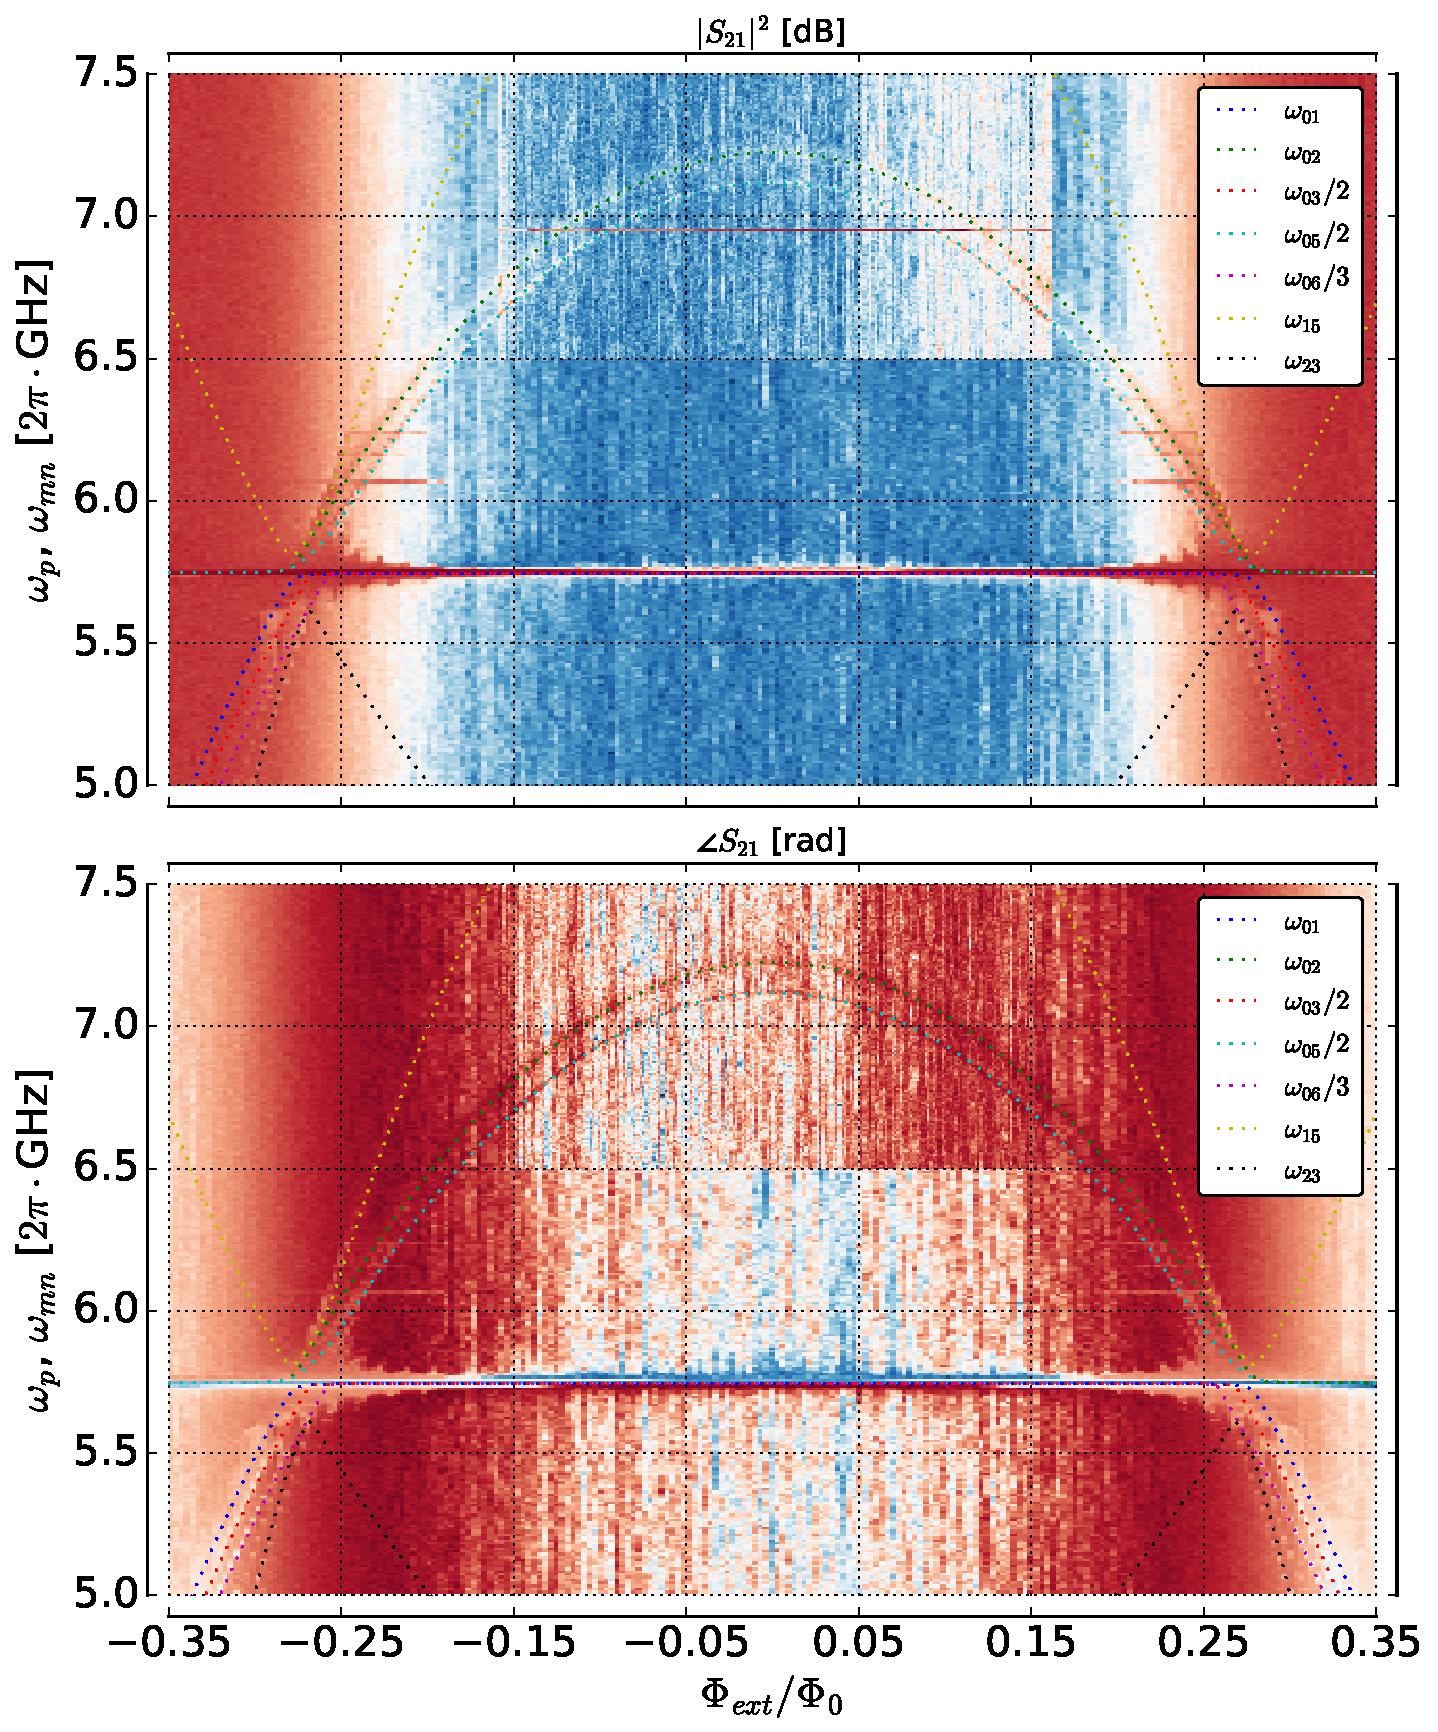
\includegraphics[width=.9\textwidth]{first_II_2tone_higher_power_fit}
\caption{The two-tone spectrum of system II at -10 dBm power level on the $\mu$-wave source with fitting lines obtained from the model \eqref{eq:hamiltonian}. More transitions are visible, new compared to \autoref{fig:first_II_2tone} are the upper branch of the two-photon $gf$ transition ($\omega_{05}/2$), the lower branch of the three-photon $gd$ transition ($\omega_{06}/3$) and also the lower branch of the sideband $\ket{1,g}\rightarrow \ket{0,f}$ ($\omega_{23}$).}
\label{fig:first_II_2tone_hp}
\end{figure}

If the power of the second tone is increased, the probability of the transitions with lesser matrix elements also rises allowing to see these transitions more clearly. Such measurement yields a spectrum as in \autoref{fig:first_II_2tone_hp}. It was done at -10 dBm; thus, a power 10 times higher than in the previous case was sent at the sample. Now the two-photon hyperbolic line $\omega_{gf}$ under the main one $\omega_{ge}$ is clearly visible (the upper complementary branch $\omega_{05}/2$ of the previously visible transition $\omega_{03}/2$). The upper branch of the sideband $\ket{1,g}\rightarrow \ket{0,f}$ is visible also, see \autoref{fig:first_II_2tone_zoom_fit} for the scan around $\Phi_{ext}=0$. Also there are two lines below the resonator at the sides of the graph whose origin is not clear. One of them might be the lower branch of that sideband (fit with $\omega_{23}$ in \autoref{fig:first_II_2tone_hp}), however it can be seen that the theoretical line is not very accurate there. The other line which is visible between $\omega_{23}$ and $\omega_{06}/3$ was not fit because no appropriate transition was found. Surely, one should be able to find it but this task looks hard enough to give it up.

	
\begin{figure}
\centering
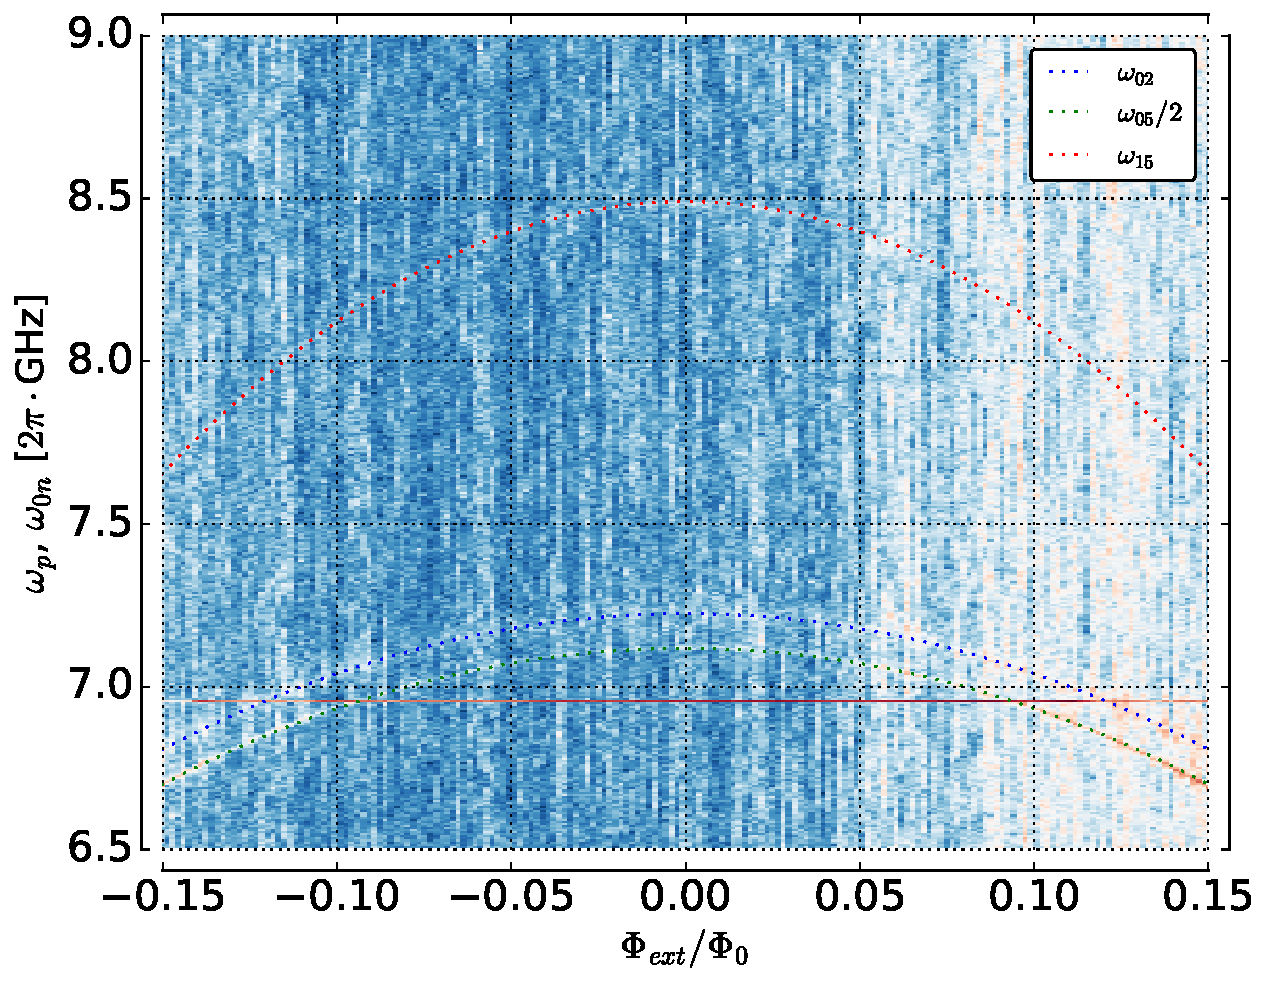
\includegraphics[width=0.8\textwidth]{first_II_2tone_zoom_fit}
\caption{Zoomed area around the main qubit transition $ge$, two-photon transition $gf$ and the sideband transition $\ket{1,g}\rightarrow \ket{0,f}$ with fitting lines. Second tone power was -10 dBm, transmission amplitude is displayed.}
\label{fig:first_II_2tone_zoom_fit}
\end{figure}

Interestingly enough as well as the transition corresponding to the system's resonator some other narrow horizontal transitions are visible. Three of these lines are visible best of all around 6.1 GHz near the qubit line in \autoref{fig:first_II_2tone}~($|S^2_{21}|$) and near 7 GHz in the high-resolution area of \autoref{fig:first_II_2tone_hp}~($|S^2_{21}|$). They correspond to the other resonators which lie higher in frequency. This effect was already observed before but was not thoroughly studied. At this moment it seems that the effect of changed transmission on the probe frequency when the other resonator is resonantly excited with large power (second tone power is 10$^4$-10$^5$ times higher than the probe power) is not due to the coupling of the resonators but due to nonlinear effects or suppressed superconductivity in the Al film itself.

\newpage

\subsubsection{System VI}

\paragraph{Model.} Below all the experimental data will be provided for system VI along with theoretical fits of the spectral lines that were observed using the model \eqref{eq:hamiltonian}. Model parameters were fit based on all data on this system and are same for all figures in this section. Before turning to the comparison of the theoretical predictions and experimental results it would be useful to present the model parameters used for fitting which are summarized in \autoref{tab:first_VI_params}.

\begin{table}[h]
\centering
\begin{tabular}{l|c}
Parameter & Value \\
\hline 
$C_\kappa$ & 0 fF \\
\hline
$C_g$ & 1.8 fF \\
\hline
$C_q$ & 95 fF \\
\hline
$E_C$ & 200 MHz
\end{tabular}~
\begin{tabular}{l|c}
Parameter & Value\\
\hline
$C_r$ & 367 fF \\
\hline
$L_r$ & 1.41 nH \\
\hline
$I_{C, \Sigma}$ & 63.4 nA \\
\hline
$E_{J, \Sigma}$ & 31.5 GHz
\end{tabular}
\caption{Values of the main parameters defining the spectrum of the model \eqref{eq:hamiltonian}.}
\label{tab:first_VI_params}
\end{table}

\paragraph{Anticrossing.} The anticrossing spectrum of the sixth system is presented in \autoref{fig:first_VI_anticrossing_fit}. It can be directly seen that the qubit is very close in frequency to its resonator; thus, the resonator line is bent slightly and the qubit line is looking ordinary. Using the theoretical model \eqref{eq:hamiltonian} these two lines were fit, and there's a good agreement between theory and data. It can be seen that at the degeneracy point, where the qubit is closest in frequency to the resonator, the resonator line becomes dimmer; it indicates that the qubit is less coherent than the resonator, reducing its Q-factor when approaching resonant interaction.

\begin{figure}
\centering
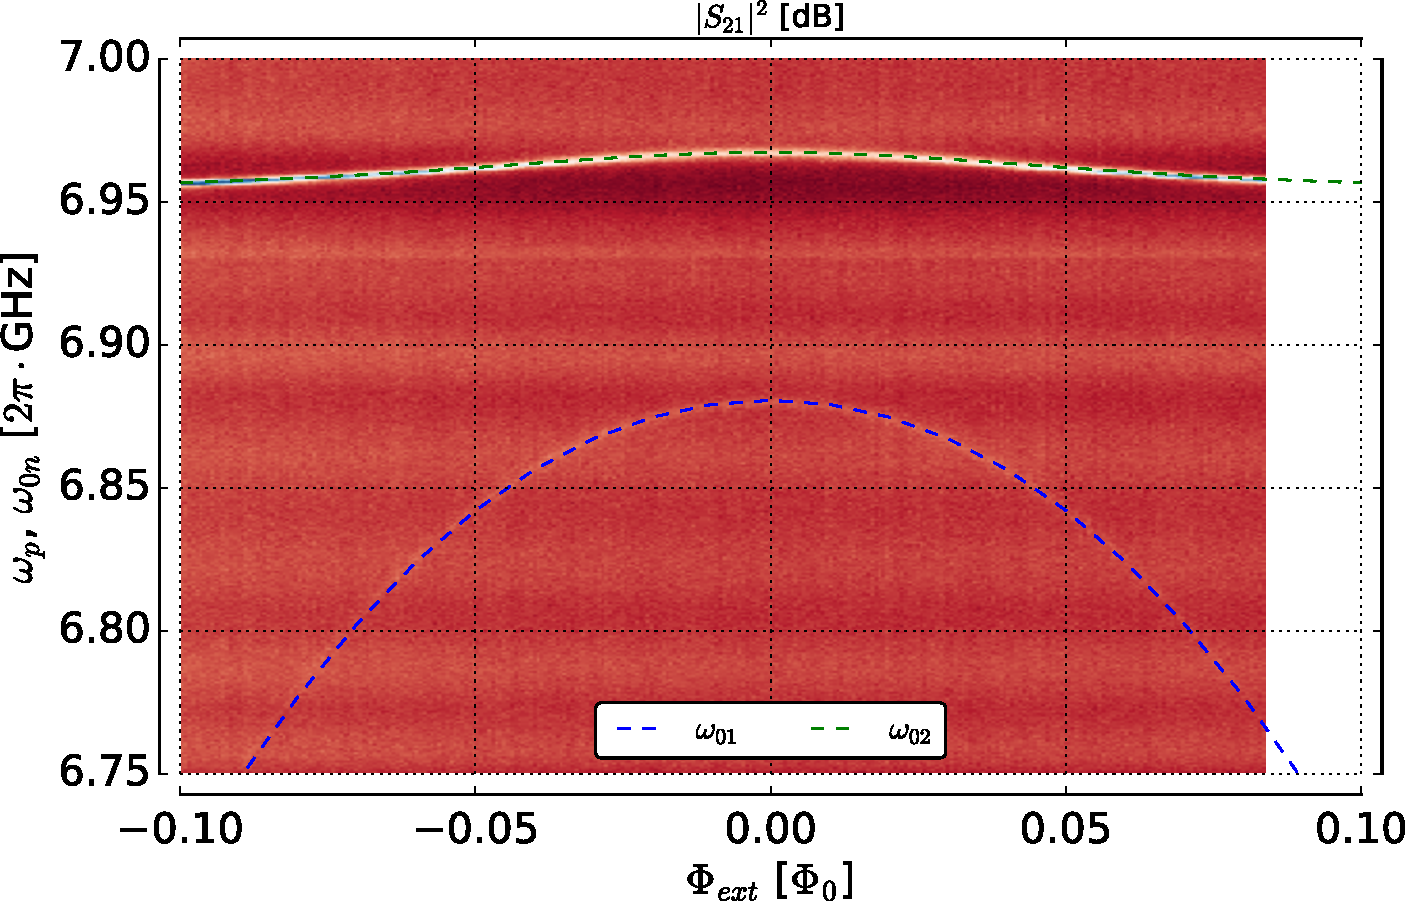
\includegraphics[width=0.9\textwidth]{first_VI_anticrossing_fit}
\caption{Anticrossing spectrum for the 6$^\text{th}$ system (z-axis normalized) with fitting lines obtained from the model \eqref{eq:hamiltonian}. }
\label{fig:first_VI_anticrossing_fit}
\end{figure}

\paragraph{Two-tone spectroscopy.} The results of the two-tone spectroscopy are presented in \autoref{fig:first_VI_2tone_fit}. It was performed at the lowest possible power of -20 dBm on the $\mu$-wave source, yet, due to a very small detuning of the qubit at the degeneracy point, the power in

\begin{figure}
\centering
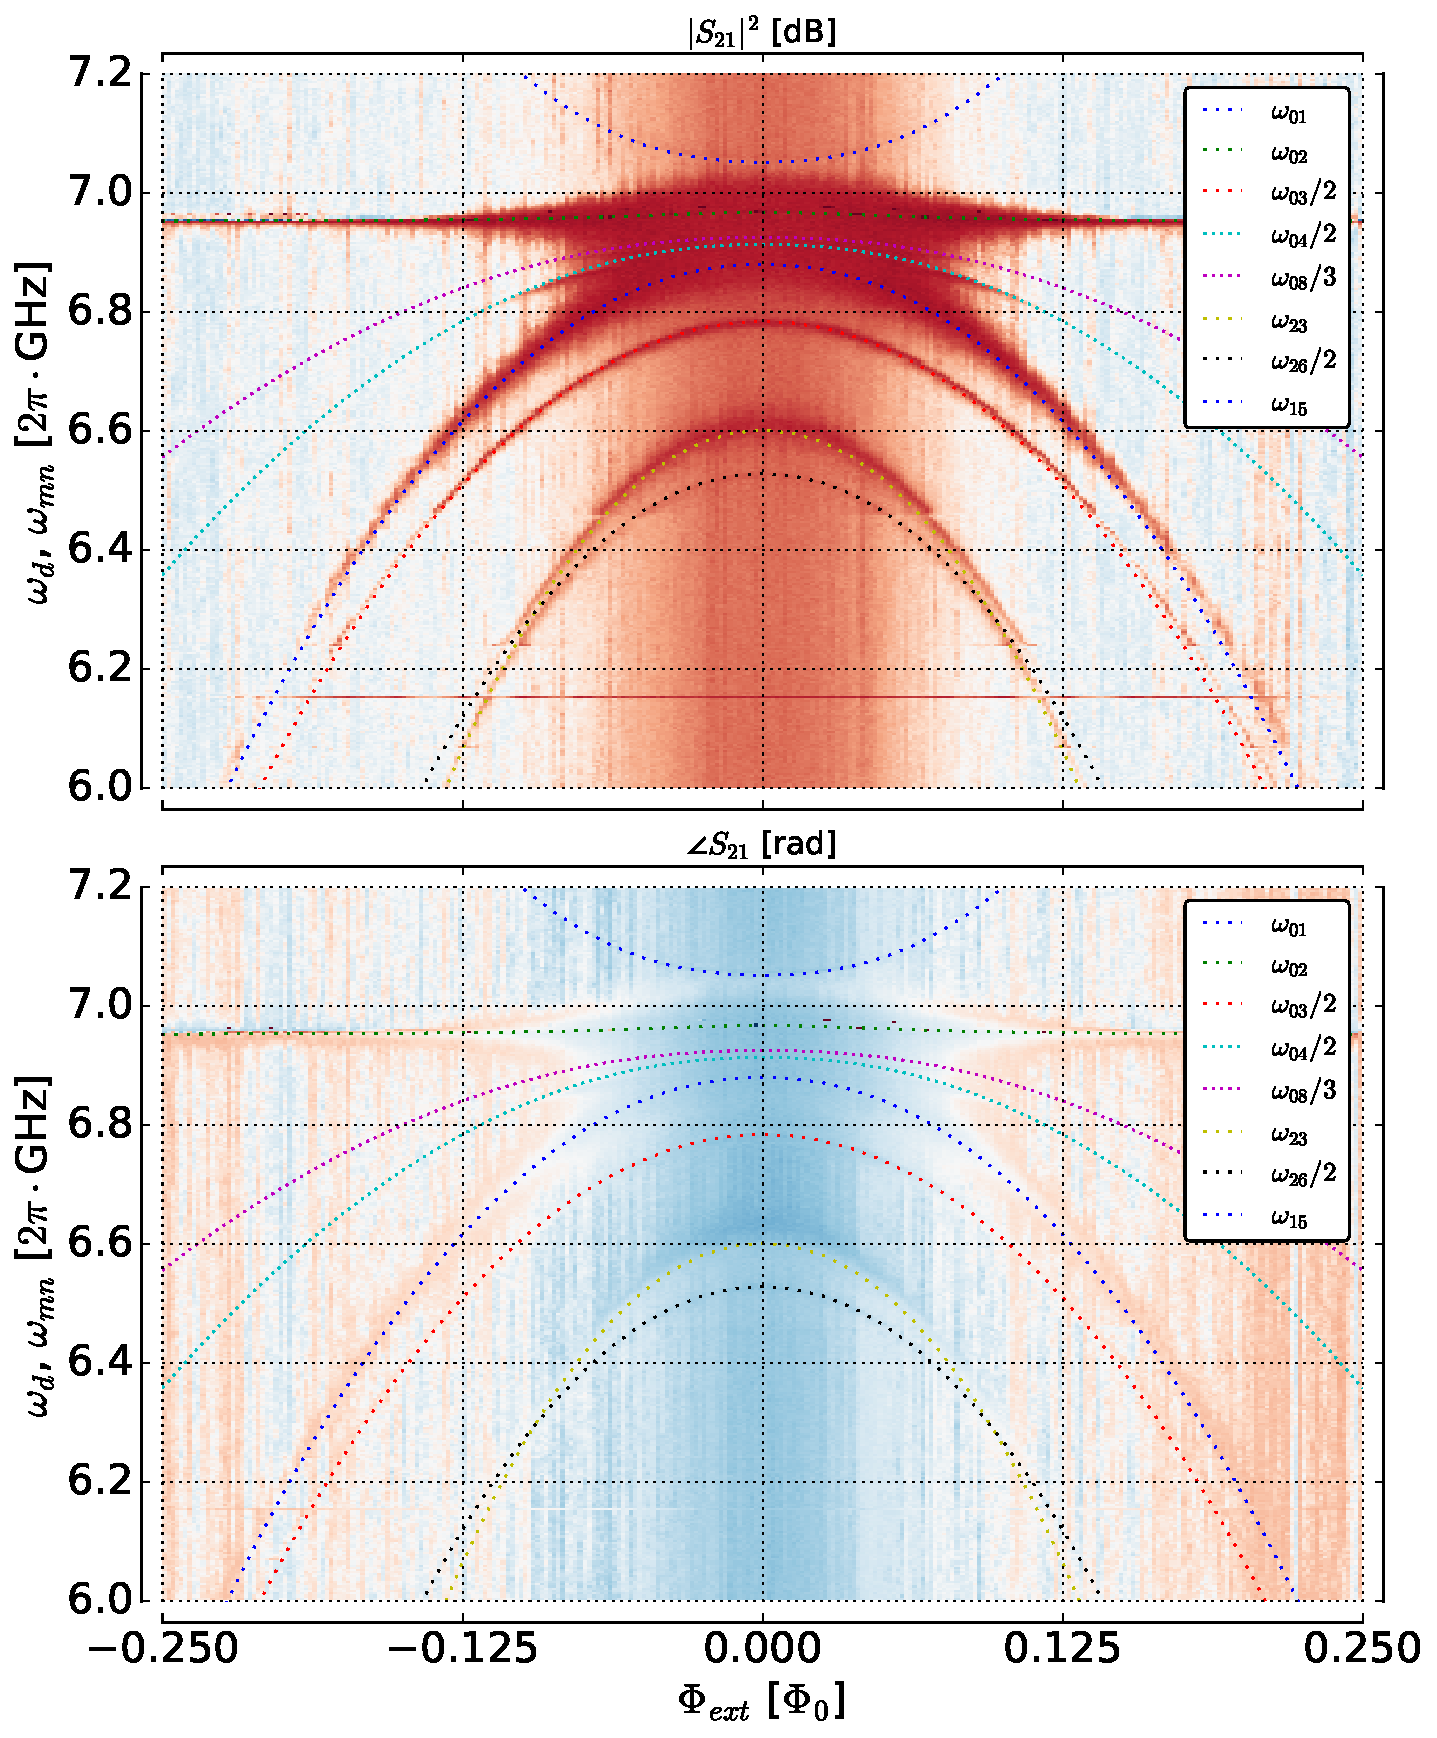
\includegraphics[width=.9\textwidth]{first_VI_2tone_fit}
\caption{Two-tone spectrum of the 6$^\text{th}$ system (z-axis normalized) at -20 dBm on the $\mu$-wave source with fitting lines obtained from the model \eqref{eq:hamiltonian}. As long as the qubit is very close to the resonator in frequency the effective driving power on it is very high, and thus a lot of sideband and multiphoton transitions are visible.}
\label{fig:first_VI_2tone_fit}
\end{figure}

\newpage

\section{On-chip control lines testing design}

\subsection{Geometry and parameters}

The second design that was developed was intended to test the properties of the control lines, i.e. flux bias lines and microwave driving lines, implemented on the chip. The design is presented in \autoref{fig:second_design_full} where some of its key features are highlighted. It's 10x5 mm.

\begin{figure}[h!]
\centering
\includegraphics[width=0.7\textwidth]{chip_design2}
\includegraphics[width=0.7\textwidth]{chip_design2_zoom}
\caption{\textbf{(a)} Large-scale image of the lines testing design. The chip (8x4 mm) consists of eight $\lambda/4$ CPW resonators coupled capacitively to the feedline, six low-Q$_e$ with Xmon qubits at the open end and two high-Q$_e$ with no qubits. \textbf{(b)} Zoomed area around one of the qubits, showing the microwave antenna configuration. \textbf{(c)} Zoomed area around another qubit, showing the flux bias line. \textbf{(d)} Zoom around one of the qubits' SQUIDs. Pink areas denote the part of the mask which produces the SQUID and should be patterned with higher resolution.}
\label{fig:second_design_full}
\end{figure}

Firstly, differently from the previous design, this design has more resonators, additional two (TI, TII, see \autoref{fig:second_design_full}(a)) were inserted at the ends of the main resonator-qubit array (I-VI). These resonators have high Q$_e$ from their geometry to yield accurate results for possible high internal Q-factors.

Secondly, the frequencies of the devices were changed. The qubits still are all calculated to have the same frequency, but it's now 6 GHz, with $C_\Sigma \approx 80$ fF and $I_{C, \Sigma} = 40$ nA. The size of each junction in the qubit's SQUID is 100x200 nm$^2$. The resonators had frequencies of 7, 7.1, 7.2, 7.3, 7.4, 7.5 GHz for the cQED systems I-VI, and the bare resonators TI and TII had 8 and 8.25 GHz, respectively.

Finally, as the main change made to the design, some coplanar control lines were introduced. For the upper qubits they are microwave antennas, i.e. open-ended coplanar line pieces, to induce transitions while for the lower qubits they are flux-bias lines to change the energy level structure of the devices. The lines were separated in such a way to make the design more fault-tolerant.

Four test structures at the sides of the chip were also included to allow direct DC measurement of the SQUIDs created during the shadow evaporation.


\begin{figure}
\centering
\includegraphics[width=0.6\textwidth]{xmon_al_bmstu_1_in_pcb}
\caption{Bonded Xmon Al BMSTU 1 in the PCB of the sample holder, as seen through the microscope of the bonding machine.}
\label{fig:first_tight_fit}
\end{figure}

\subsection{Implementation and purposes}

The chip Xmon Al BMSTU 1 was made in a single-step process. It had a mask patterned with e-beam in the cleanroom facility at Bauman Moscow State Technical University (add recipe?), and then Al film was shadow-evaporated on Plassys in the RQC lab in ISSP, 25 and 45 nm thick. The substrate used was made of high-resistivity Si ($> 6$ kOhm/cm).

One significant difference about this sample is that in fact it was fabricated with its twin in the center of a larger substrate (15x15 mm) which was previously patterned on the back side with a circular saw to allow the substrate to be cracked around the chips precisely. However, the process wasn't yet mastered, and the twin chip was lost during the separation. But nevertheless, the remaining sample fitted in the PCB cutout really well (see \autoref{fig:first_tight_fit}), and the method will be further improved.


Purposes for the design:
\begin{enumerate}[label=(\alph*), leftmargin=1.5cm]
\itemsep0pt
\item to test resonator Q without qubits

\item to test lines

\item to test again the qubits' basic parameters

\item to test improvement of the noise

\item to test the half-sawing of the sample with following cracking
\end{enumerate}

\subsection{Measurement setup  STUBBED from first chip, needs review}

The sample was measured at ISSP in laboratory of RQC. Cryogenic equipment was represented by BlueFors LD250 dilution refrigerator, with base temperature of 16 mK. The microwave equipment included R\&S ZNB 10 kHz-20 GHz vector network analyser,  Agilent E8257D 100 kHz - 40 GHz analog signal generator. The sample was flux biased using Keithley 6221 current source.

Microwave line was thermalized with 60 dB of attenuation, additional 20 dB of attenuation were introduced on a directional coupler which added the second tone from the $\mu$-wave source. After leaving the sample the signal passed through two isolators and a hybrid coupler, which was used before to measure two samples during single cooldown. Finally, the signal was amplified with 4-8 GHz LNF amplifier at 4 K and a with a room-temperature amplifier.

The sample holder that was used was designed for 10x10 mm chips, so the bondwires had a relatively large length of 1 mm which of course deteriorated the overall transmission. Chip lay directly on the copper disk of the bottom part of the sample holder with no hole carved under it. Around the sample holder a superconducting coil was wound which has been supplied using the current source mentioned above.

The magnetic shielding of the sample holder was achieved via a cryoperm shield. A superconducting shield was not installed in this run due to the lack of space inside the magnetic shield, which may have influenced the noise background.

\begin{figure}[h!]
\centering
\includegraphics[width=0.9\textwidth]{xmon_al_bmstu_1_general}

\includegraphics[width=0.9\textwidth]{xmon_al_bmstu_1(2)_general}

\includegraphics[width=0.9\textwidth]{xmon_al_bmstu_1(3)_general}


\caption{\textbf{(Top)} General view of the resonances. All six resonances are visible, however shifted down in frequency. This shift more or less consistent throughout the devices, and thus it's most probably caused by effective $\epsilon_{Si}$ different from the one used in the calculation. \textbf{(Middle)} General view of the resonances (2$^\text{nd}$ cooldown). Transmission now lower as a 5 dB attenuator was replaced by a 10 dB one. Seven resonances are visible, as the second resonator presumably coupled to something. The shapes of the other peaks also changed. \textbf{(Bottom)} General view of the resonances (3$^\text{d}$ cooldown).  Transmission is 20 dB higher as the directional coupler was altered. Again, six resonances are visible, though some spurious dip is present between devices III and IV, and the shapes changed again.}
\label{fig:second_resonators_general}
\end{figure}


\begin{figure}[h!]
\centering

\includegraphics[width=\textwidth]{q-factors-and-freqs_xmon_al_bmstu_1}

\caption{Various quality factors and frequencies depending on radiation power. Some resonators show interesting dip in internal Q near -25 dBm and significant change in frequency, implying they are coupled to functioning qubits saturation of which causes the effect. Other resonators do not show such features.}
\label{fig:second_q_factors}
\end{figure}

\begin{figure}[h!]
\centering
\includegraphics[width=\textwidth]{q-factors-and-freqs_xmon_al_bmstu_1(2)}
\caption{Same figure for the 2$^\text{nd}$ cooldown. Significant deviations are present in comparison with the first cooldown, both to the greater and to the lower Q-factors on different devices.}
\label{fig:second_q_factors(2)}
\end{figure}

\begin{figure}[h!]
\centering
\includegraphics[width=\textwidth]{q-factors-and-freqs_xmon_al_bmstu_1(3)}
\caption{Same figure for the 3$^\text{d}$ cooldown. The Q-factors degraded completely both for the cQED resonators and the test resonators.}
\label{fig:second_q_factors(3)}
\end{figure}

\subsection{Characterization of the resonators}

The resonators on the sample were measured several times (after each new cooldown) as they seemed to degrade. Indeed, looking at the Q-factors over the cooldowns reveals that the resonators got worse and worse, even if nothing at all was done with the chip.

Before the second cooldown the chip was moved out of the PCB to solder additional SMP connectors on it, and then moved back in. No mechanical damage or contamination was inflicted to it. However, we can see dramatic changes in quality factors of the resonators, some got better and some got worse for unknown reasons (see \autoref{fig:second_q_factors(2)}). Devices II and III got so bad it was impossible to fit them as their widths compare to the S$_{12}$ general roughness features (see \autoref{fig:second_resonators_general} (Top) vs (Middle)).

After that before the third cooldown nothing at all was done to the chip. After the cooldown and before the Q-factor measurement there was an accidental excessive current through the surrounding coil. Though, it didn't change the general appearance of the resonances which was again found different at this cooldown (see \autoref{fig:second_resonators_general} (Bottom)). At this run the Q-factors became unacceptably low (see \autoref{fig:second_q_factors(3)}) at all powers. 


\subsection{Characterization of the cQED systems}

The two systems were possible to study in this sample, I and VI. Others either did not indicate presence of the functional qubits or experience strong flux hopping while tuned via the superconducting coil and don't have the flux bias lines attached to work around this problem. Fortunately, system I has the qubit with the flux bias line and system VI has the microwave antenna, so both these on-chip devices were successfully tested.



\subsubsection{System I}

The system one was biased by the superconducting loop right on the chip. This allows to make wide scans without affecting negatively the resonator with the width limited only by the current source. The periodic spectrum of the anticrossings for system I is displayed in \autoref{fig:second_I_anti}. The pattern is shifted noticeably to the left due to some residual field around the sample.

\begin{figure}[h]
\centering
\includegraphics[width=\textwidth]{second-I-anti}
\caption{Periodic anticrossing picture for the system I (at high power). The current on the current source spans 80 mA and is actually comparable at the endpoints to it's maximum possible output of 105 mA.}
\label{fig:second_I_anti}
\end{figure}

\begin{figure}[h]
\centering
\includegraphics[width=\textwidth]{second-I-spec-lines}

\includegraphics[width=\textwidth]{ge-linewidth}
\caption{Qubit spectrum at 0 dBm on the output of the 2$^{\text{nd}}$ tone generator (left), dependence of the linewidth on the driving power (right) and high-resolution scan of the two-tone peak at -20 dBm (bottom).}
\label{fig:second_I_spec_lines}
\end{figure}


The experiment to determine qubit spectrum and the linewidth at the degeneracy point was also done on the system. The resulting graphs are presented in \autoref{fig:second_I_spec_lines}. On the right plot the spectrum of the qubit is visible; it consists of three lines corresponding to the transitions $ge,\ gf/2$ and $gd/3$ and visible due to the high power of the drive. On the left plot the spectral line width is recorded over the incident power of the drive. It's possible to estimate the linewidth of the bare qubit from the phase 2-tone data (see Section \ref{sec:2tone}). The line experiences significant broadening with increased power; though, at the minimal possible power of -20 dBm it's width is very small, around 0.5 MHz, which allows to set a lower bound of 300 ns on the qubit $T_1$ (assuming that there's no pure dephasing due to the flux fluctuations at the sweet spot and to the excessive population of the resonator as $\delta\omega = \frac{1}{T_1}+\frac{2}{T_2}$).

\subsubsection{System VI}

System VI had an on-chip microwave antenna nearby, but had no flux bias line (see \autoref{fig:second_design_full}), and thus had to be biased by the external coil. With the studied sample this method of biasing was very inconvenient, as even small magnetic field from the coil influenced the resonators tremendously, inducing continuous and discontinuous frequency shifts in them, presumably due to flux creep and hopping. Fortunately, is was still possible to tune the qubit of the VI$^{\text{th}}$ system enough to observe it's spectrum and to test the microwave antenna.

\begin{figure}
\centering
\includegraphics[width=0.7\textwidth]{second_VI_anti}
\caption{Anticrossing of the VI$^{\text{th}}$ cQED system. It can be seen that the picture is not symmetric and   the lines are bent downwards at the ends, as the resonator frequency change was caused not only by the qubit, but also directly by the magnetic field.}
\label{fig:second_VI_anti}
\end{figure}

The anticrossing measured for this system is shown in \autoref{fig:second_VI_anti}. It was hard to measure, though, as the flux hopping was interfering with the tuning of the qubit. The resonator frequency change due to the magnetic field has bent the picture, so it would be impossible to fit it within the model described before. Nevertheless, the spectrum of this qubit was gathered with 2-tone spectroscopy using the microwave antenna and with a second tone driving the resonator. The results are presented in \autoref{fig:second_VI_spec_antenna} for the measurement via an antenna and with an additional tone in the feedline driving the resonators at the qubit's frequency.

\begin{figure}[h]
\includegraphics[width=\textwidth]{second_VI_spec_antenna}
\caption{Two-tone spectroscopy of the VI$^{\text{th}}$ system using the microwave antenna mounted on the chip.}
\label{fig:second_VI_spec_antenna}
\end{figure}

\begin{figure}[h]
\includegraphics[width=\textwidth]{second_VI_spec}
\caption{Two-tone spectroscopy of the VI$^{\text{th}}$ system using the directional coupler to add the second tone to the probe line. The background was subtracted. It can be seen also where the flux jumped abruptly: it happened near 0.5 mA and resulted in a decrease of the field penetrating the qubit's SQUID.}
\label{fig:second_VI_spec_antenna}
\end{figure}

\appendix

\chapter{Pure dephasing or Does the density matrix really exist?}

There are two ways of describing pure dephasing. One is developed from the system-bath approach (Lindbladian master equation) and the other comes from the stochastic Schrödinger equation. However, the results of the latter deviate fundamentally from the results of the former for the experiment of spin-echo for a single qubit. Here this problem will be described in detail.

\section{Quantum derivation of dephasing}

For the derivation of this phase-destroying process in a quantum way the system-environment interaction Hamiltonian part is chosen as
\[
\mathcal{\hat H}_{qe} = \hat \sigma_z \otimes \hat O_e, 
\]
where $\hat O_e$ is an arbitrary environment operator. From this interaction term a master equation is then developed:
\[
\partial_t \hat \rho_s = \frac{i}{\hbar}[\hat \rho_s, \mathcal{\hat H}_s] + \frac{\gamma_\phi}{2} (\hat \sigma_z \hat \rho_s \hat \sigma_z - \hat \rho_s).
\]
The dynamics of this equation can be seen in \autoref{fig:qdeph}.  At $t \rightarrow \infty$ the state of the system is a totally mixed state:
\[
\hat \rho_s (\infty) = \rbrkt{\begin{matrix}
\rho_{11}(0) & 0 \\
0 & \rho_{22}(0) 
\end{matrix}}.
\]
Following the open system approach this should be understood as the consequence of the entanglement of the qubit with the environment. The same density matrix we will obtain trying to find out in which state
is the qubit $A$ when it's a part of a composite system $A \otimes B$ of two qubits being in a Bell  state $\ket{\Psi^+} = \frac{1}{\sqrt{2}}(\ket{0}_A\otimes\ket{1}_B+\ket{1}_A\otimes\ket{0}_B)$. From the quantum point of view, therefore, the process of dephasing is irreversible.
\begin{figure}
\centering
\begin{subfigure}[t]{0.45\textwidth}
\centering
\includegraphics[width=0.9\textwidth]{qdeph_bloch}
\caption{Dephasing on the Bloch sphere.}
\end{subfigure}
\begin{subfigure}[t]{0.45\textwidth}
\centering
\includegraphics[width=0.9\textwidth]{qdeph_bloch_rf}
\caption{Same within the rotating frame.}
\end{subfigure}

\begin{subfigure}[t]{0.45\textwidth}
\centering
\includegraphics[width=0.9\textwidth]{qdeph_xyz}
\caption{Decay of the $\langle \hat \sigma_{x, y} \rangle$ components.}
\end{subfigure}
\begin{subfigure}[t]{0.45\textwidth}
\centering
\includegraphics[width=0.9\textwidth]{qdeph_xyz_rf}
\caption{Same within the rotating frame.}
\end{subfigure}
\caption{Dephasing treated quantum-mechanically shows exponential decrease of the coherences of the density matrix.}
\label{fig:qdeph}
\end{figure}

\section{Classical derivation of dephasing}

The classical derivation will be presented below in detail. This method, just as in the case of interaction of an atom with a classical field, just includes an additional time-dependent term in the Hamiltonian, representing fluctuations of the system's parameters. For the pure dephasing this term looks like $f(t) \hat \sigma_z$, where $f(t)$ is the random noise. It is possible to write down the evolution of the density matrix for such stochastic Schrödinger equation. Until specified, the unitary evolution will be discussed, although using density matrix. In the rotating frame:
\[
\hat \rho_s (t) = \hat U^\dag(t, 0)\ \hat\rho\ \hat U(t, 0), 
\]
where 
\[
\hat U(t, 0) = \hat T \exp \left\{-\frac{i}{\hbar} \int_0^t f(\tau)\hat \sigma_z \diff\tau\right\}.
\]
From the fact that $\hat \sigma_z$ is diagonal it can be shown that
\[
\begin{gathered}
\hat \rho_s (t) = \rbrkt{\begin{matrix}
\exp \left\{\frac{i}{\hbar} \int_0^t f(\tau_1) \diff\tau_1\right\} & 0\\
0 & \exp \left\{-\frac{i}{\hbar} \int_0^t f(\tau_1) \diff\tau_1\right\}
\end{matrix}}\cdot\\
\cdot\rbrkt{\begin{matrix}
1/2 - N(0)/2 & \rho(0) \\
\rho^*(0) & 1/2 + N(0)/2 
\end{matrix}}\cdot\\
\cdot\rbrkt{\begin{matrix}
\exp \left\{-\frac{i}{\hbar} \int_0^t f(\tau_2)\diff\tau_2\right\} & 0\\
0 & \exp \left\{+\frac{i}{\hbar} \int_0^t f(\tau_2)\diff\tau_2\right\}
\end{matrix}},
\end{gathered}
\] 
where the integral variables $\tau_1$ and $\tau_2$, coherence $\rho(t)$ and inversion $N(t)$ were introduced. From above it is obvious that
\begin{gather}
N(t) = N(0),\\
\rho(t) = \rho(0)\exp \left\{ \frac{2i}{\hbar}\int_0^t f(\tau)  \diff \tau \right\}. \label{eq:rho_t}
\end{gather}
This equations can be visualized with numerical simulation, taking $f(t)$ be, for instance, normally distributed. The phase will experience random drifts, which lead to random rotations of the Bloch vector on the equator of the sphere, see \autoref{fig:cdeph}~(a), (c).

However, we can now use the other side of the density matrix, the property for which it is also called statistical operator. Let's run the equation \eqref{eq:rho_t} many times and look at the statistically expected state of the observed system over time. The diagonal part will still stay the same, and for coherence we have (presuming Gaussian instantaneous distribution of $f(t)$ and $x(t) = \frac{2}{\hbar}\int_0^t f(\tau)  \diff \tau$):
\begin{gather}
\langle \rho(t) \rangle = \rho(0) \int_{-\infty}^{+\infty} e^{ix}\, \mathbb{N}_{0,\sigma}(x) \diff x = \rho(0) e^{-\sigma^2/2} = \rho(0) e^{-\langle x^2 \rangle/2} \\
= \rho(0)\exp \left\{ -\frac{2}{\hbar^2}\int_0^t\int_0^t \langle f(\tau_1) f(\tau_2) \rangle \diff \tau_1 \diff \tau_2 \right\}.
\end{gather}
Presuming also that $f(t)$ is a wide-sense stationary process $\langle f(\tau_1) f(\tau_2) \rangle = K_f(\tau_2 - \tau_1) = \frac{1}{\sqrt{2\pi}}\int\limits_\mathbb{R} S_f(\omega) e^{i\omega(\tau_2-\tau_1)}\diff\omega$ where $S_f(\omega)$ is the power spectral density of $f(t)$. Taking the time integrals with the exponents, finally we obtain
\begin{equation}
\langle \rho(t) \rangle = \rho(0) \exp  \left\{-\frac{2}{\sqrt{2\pi}\hbar^2} \int\limits_\mathbb{R} W_t^R(\omega) S_f(\omega)\diff \omega \right\},\  W_t^R(\omega)  = \frac{4 \sin^2(\frac{\omega t}{2})}{\omega^2}\label{eq:cdeph}
\end{equation}
It can be shown easily that \eqref{eq:cdeph} is an exponent for either a white noise ($S_f(\omega) = S_f(0) = const$) or for a sufficiently large time $t$ where 
$$\frac{t}{2}\int\limits_\mathbb{R} \diff(\omega t/2) \frac{\sin^2(\frac{\omega t}{2})}{(\omega t/2)^2} \ \bullet $$
acts as $ \frac{t\pi}{2}\delta(\omega)\ \bullet$. In both these cases the pure dephasing rate $\Gamma^*_2$ exists in the usual sense and $\Gamma^*_2 \propto S_f(0)$. In case of, for example, the 1/f noise, the decay curve will behave as $e^{-t^2}$ in the vicinity of $t=0$.

The averaged evolution for the white noise case can be observed in \autoref{fig:cdeph}~(b), (d). It is very similar to what can be seen in \autoref{fig:qdeph}. 1000 trajectories were used for averaging.
In \autoref{fig:cdeph_pink} the simulation of the dynamics under the 1/f noise is shown. For the averaged case ((b), (d)) 2500 trajectories where used. One can see that a plateau is present for the yellow graph near $t=0$, in accordance with theoretical predictions.
\begin{figure}
\begingroup
\captionsetup[subfigure]{width=0.9\textwidth}
\centering
\begin{subfigure}[t]{0.45\textwidth}
\centering
\includegraphics[width=0.9\textwidth]{cdeph_bloch_rf}
\caption{White Gaussian noise affecting the phase in the rotating frame.}
\end{subfigure}
\begin{subfigure}[t]{0.45\textwidth}
\centering
\includegraphics[width=0.9\textwidth]{cdeph_bloch_rf_avg}
\caption{Averaged dynamics in the rotating frame.}
\end{subfigure}

\begin{subfigure}[t]{0.45\textwidth}
\centering
\includegraphics[width=0.9\textwidth]{cdeph_xyz_rf}
\caption{Behaviour of the $xyz$ components in the rotating frame.}
\end{subfigure}
\begin{subfigure}[t]{0.45\textwidth}
\centering
\includegraphics[width=0.9\textwidth]{cdeph_xyz_rf_avg}
\caption{Averaged behaviour of the $xyz$ components in the rotating frame.}
\end{subfigure}
\caption{Classically treated pure dephasing for white noise.}
\label{fig:cdeph}
\endgroup
\end{figure}

\begin{figure}
\begingroup
\captionsetup[subfigure]{width=0.9\textwidth}
\centering
\begin{subfigure}[t]{0.45\textwidth}
\centering
\includegraphics[width=0.9\textwidth]{cdeph_bloch_rf_pink}
\caption{1/f Gaussian noise affecting the phase in the rotating frame.}
\end{subfigure}
\begin{subfigure}[t]{0.45\textwidth}
\centering
\includegraphics[width=0.9\textwidth]{cdeph_bloch_rf_avg_pink}
\caption{Averaged dynamics in the rotating frame.}
\end{subfigure}

\begin{subfigure}[t]{0.45\textwidth}
\centering
\includegraphics[width=0.9\textwidth]{cdeph_xyz_rf_pink}
\caption{Behaviour of the $xyz$ components in the rotating frame.}
\end{subfigure}
\begin{subfigure}[t]{0.45\textwidth}
\centering
\includegraphics[width=0.9\textwidth]{cdeph_xyz_rf_avg_pink}
\caption{Averaged behaviour of the $xyz$ components in the rotating frame.}
\end{subfigure}
\caption{Classically treated pure dephasing for 1/f noise.}
\label{fig:cdeph_pink}
\endgroup
\end{figure}

\begin{figure}
\centering
\includegraphics[width=0.4\textwidth]{ramsey_filter}\quad
\includegraphics[width=0.4\textwidth]{hahn_filter}
\caption{Qualitative plot for noise PSD filtration at $t=10$ s.}
\end{figure}

\section{Spin-echo experiment}

The spin-echo experiment in the simplest case (Hahn echo) is a modification of a Ramsey pulse sequence with an additional $\pi_y$-pulse right in between the $\frac{\pi}{2}_x$ ones. The idea is that during the second period (after the $\pi_y$-pulse)  slow components of the noise will cancel out the phase difference they've imposed during the first period. This can be understood easily in the limit of constant noise and infinitely fast rotations. There are also more sophisticated echo sequences such as CP, CPMG and UDD\cite{Bylander2011} which use more than one $\pi_y$-pulse during the free evolution; however, for our case it is enough to regard the simplest Hahn echo.

Mathematically Hahn echo within the previous formulations acts as follows. Before the  $\pi_y$-pulse at time $t/2$ we have the same dynamics described by \eqref{eq:rho_t}. Then, instantaneously, the coherences of the density matrix are complex conjugated as a result of an infinitely fast $\pi_y$-pulse. This can be understood from the result of $\pi_y$-pulse on the Bloch sphere: $\left< \hat \sigma_x \right> = \rho + \rho^* \overset{\pi_y}{\rightarrow}  \left< \hat \sigma_x \right>,\ \left< \hat \sigma_y \right> = i(\rho - \rho^*) \overset{\pi_y}{\rightarrow} -\left< \hat \sigma_y \right>,\ \left< \hat \sigma_z \right> = N  \overset{\pi_y}{\rightarrow}  \left< \hat \sigma_z \right>$. Finally, for the changed initial condition at $t/2$ again evolution \eqref{eq:rho_t} is applied. Therefore, at the end of the period the coherence is defined as
\begin{equation*}
\rho(t) = \rho(0)\exp \left\{ - \frac{2i}{\hbar}\int_0^{t/2} f(\tau)  \diff \tau + \frac{2i}{\hbar}\int_{t/2}^{t} f(\tau)  \diff \tau \right\}.
\end{equation*}
Performing the ensemble averaging one can get
\begin{gather*}
\left<\rho(t)\right> = \rho(0)\exp \left\{ - \frac{2}{\hbar^2} \left< \left( \int_0^{t/2} f(\tau_1)  \diff \tau_1 + \int_{t/2}^{t} f(\tau_2)  \diff \tau_2 \right)\cdot \right. \right. \\
\cdot \left. \left. \left( \int_0^{t/2} f(\tau_3)  \diff \tau_3 + \int_{t/2}^{t} f(\tau_4)  \diff \tau_4 \right) \right> \right\}.
\end{gather*}
Expanding the brackets, again putting a Fourier transform of the power spectral density $S_f(\omega)$ instead of the autocorrelation functions and factoring the expression back to the initial representation it is possible to obtain\cite{Preskill} the final expression for the coherence expectation:
\begin{equation}
\left<\rho(t)\right> = \rho(0)\exp \left\{ - \frac{2}{\sqrt{2\pi} \hbar^2} \int_\mathbb{R} S_f(\omega) W^H_t (\omega) \diff\omega \right\},
\label{eq:cdeph_se}
\end{equation}
where
\begin{align*}
 W^H_t (\omega)  &= \left| - \int_0^{t/2} e^{i \omega \tau}\diff \tau + \int_{t/2}^{t} e^{i\omega\tau}  \diff \tau  \right|^2 \\
& =  \left| 1-2e^{i\omega t/2} + e^{i\omega t} \right| \\
&= \left| \frac{(1-e^{i\omega t/2})}{(1+e^{i\omega t/2})} (1+e^{i\omega t/2})(1-e^{i\omega t/2})\right|\\
& = \tan^2(\omega t/4)\frac{4 \sin^2(\omega t/2)}{\omega^2}.
\end{align*}
It's obvious from \eqref{eq:cdeph_se}  that the noise influence is now suppressed at low frequencies (compare with \eqref{eq:cdeph}) however it is enhanced at some higher frequency. This leads to inefficiency of Hahn echo and similar techniques when the noise is white and a good $T_2^*$ improvement when it's 1/f, see \autoref{fig:cdeph_both}.


\begin{figure}
\begingroup
\captionsetup[subfigure]{width=0.9\textwidth}
\centering
\begin{subfigure}[t]{0.45\textwidth}
\centering
\includegraphics[width=0.9\textwidth]{deph_white}
\end{subfigure}
\begin{subfigure}[t]{0.45\textwidth}
\centering
\includegraphics[width=0.9\textwidth]{deph_pink}
\end{subfigure}

\begin{subfigure}[t]{0.45\textwidth}
\centering
\includegraphics[width=0.9\textwidth]{deph_white_se}
\end{subfigure}
\begin{subfigure}[t]{0.45\textwidth}
\centering
\includegraphics[width=0.9\textwidth]{deph_pink_se}
\end{subfigure}
\caption{Decoherence under white (left) and 1/f (right) noises with (bottom) and without (top) a refocusing $\pi_y$-pulse.}
\label{fig:cdeph_both}
\endgroup
\end{figure}

\section{The problem (of Markovian MEs)}

The interesting correspondence between quantum and classical derivation can be noted within the spin echo experiment. For the white noise both of the descriptions yield same results, the exponential decay of coherences with an equal rate. However the meanings of these two results are completely different. Quantum approach tells us that the density matrix will emerge even in a single experiment as a consequence of entanglement with the environment. Classical approach tells us that everything that  happens to the system in a single experiment is unitary, and if we knew the noise beforehand, we would be able to find out what state the qubit ended his evolution in at every final time $t$. Classical description only knows that the noise is white, non-correlated -- and this same idea is used in the derivation of the master equation when Markov approximation is applied.

This correspondence is lucky, but what happens if the noise \textit{is} correlated? The classical model now allows for (at least partially) reversible dynamics. In contrast, the entanglement process is completely irreversible, so the quantum model should not simply entangle the system with the environment for the correlated bath.

At this point it is safe to say that density matrix really exists (that means it is not just a way to describe statistical distribution of states, but is the only approach to describe an open quantum system), but the quantum model of decoherence for the correlated noise should go beyond the Markovian master equations to keep up with experiments and naive (but still correct!) classical description.\cite{Zurek2003}

\begin{figure}
\begingroup
\captionsetup[subfigure]{width=0.9\textwidth}
\centering
\begin{subfigure}[t]{0.45\textwidth}
\centering
\includegraphics[width=0.9\textwidth]{cse_bloch_rf}
\caption{Schrödinger equation solution with driving and classical dephasing caused by the single $S(0)$ spectral component of the noise.}
\end{subfigure}
\begin{subfigure}[t]{0.45\textwidth}
\centering
\includegraphics[width=0.9\textwidth]{qse_bloch_rf}
\caption{Master equation solution with driving and quantum dephasing.}
\end{subfigure}

\begin{subfigure}[t]{0.45\textwidth}
\centering
\includegraphics[width=0.99\textwidth]{cse_xyz_rf}
\caption{Same in $xyz$. Dephasing is linear in time and reversible for this case.}
\end{subfigure}
\begin{subfigure}[t]{0.45\textwidth}
\centering
\includegraphics[width=0.99\textwidth]{qse_xyz_rf}
\caption{Same in $xyz$. Dephasing destroys the coherence and is irreversible.}
\end{subfigure}
\caption{Classical versus quantum spin-echo experiment modelling. Spin-echo can't cope with quantum noise.}
\label{fig:se}
\endgroup

\end{figure}

\bibliographystyle{ugost2008}
\bibliography{report.bib}
\end{document}
